\documentclass[11pt,a4paper]{report}
\usepackage[margin=1.2in]{geometry}
\usepackage{graphicx}
\usepackage{csquotes}
\usepackage{rotating}
\usepackage{amsmath}
\usepackage{algorithm}
\usepackage{mathtools}
\usepackage[noend]{algpseudocode}
\usepackage[justification=centering]{caption}
\usepackage[export]{adjustbox}
\usepackage{listings}
\usepackage{color}

\definecolor{dkgreen}{rgb}{0,0.3,0}
\definecolor{gray}{rgb}{0.5,0.5,0.5}
\definecolor{mauve}{rgb}{0.58,0,0.82}

\lstset{frame=tb,
  language=Java,
  aboveskip=3mm,
  belowskip=3mm,
  showstringspaces=false,
  columns=flexible,
  basicstyle={\small\ttfamily},
  numbers=none,
  numberstyle=\tiny\color{gray},
  keywordstyle=\color{blue},
  commentstyle=\color{dkgreen},
  stringstyle=\color{mauve},
  breaklines=true,
  breakatwhitespace=true,
  tabsize=3
}

% Aberstwyth dissertation LaTeX Template
% Authors: Dr. Hannah Dee (hmd1@aber.ac.uk), Neil Taylor (nst@aber.ac.uk)
% This has been adapted from the Leeds Thesis template and the 
% Group Project template for Computer Science in Aberystywth University.
% 
% All comments and suggestions welcome.
%
% Template designed to be used with pdflatex: it may need alteration to
% run with a different LaTeX engine

% To build document on the unix command line, run four commands:
 
% pdflatex dissertation
% bibtex dissertation
% pdflatex dissertation
% pdflatex dissertation

% you will end up with dissertation.pdf 
\usepackage{mmp}

% the following packages are used for citations - You only need to include one. 
%
% Use the cite package if you are using the numeric style (e.g. IEEEannot). 
% Use the natbib package if you are using the author-date style (e.g. authordate2annot). 
% Only use one of these and comment out the other one. 
\usepackage{cite}
%\usepackage{natbib}

% Use the following to selectively exclude chapters
%\includeonly{cover,abstract,acknowledge,declare,chapter1,chapter2}

\begin{document}

% all of the include directives below refer to tex files
% so 
\title{Visualisng Ant Colony Optimisation}

% Your name
\author{Christopher Edwards}
% Your email 
\authoremail{che16@aber.ac.uk}

\degreeschemecode{G400} %e.g. G400 
\degreeschemetitle{Computer Science} % e.g. Computer Science
\degreetype{BSc}

\modulecode{CS39440} % i.e. CS39440, CC39440, CS39620
\moduletitle{Major Project} % i.e. Major Project or Minor Project

\date{\today} % i.e. the date of this version of the report

\status{Draft} % Use draft until you create the release version. Then, change this to Release.
\version{1.0}

%The title and name of your supervisor.
\supervisor{Dr. Neil MacParthalain} 

%The email for your supervisor. 
\supervisoremail{ncm@aber.ac.uk}

\maketitle



 includes cover.tex - to change the content,
% edit the tex file

\pagenumbering{roman}

% This is the front page

\title{Visualisng Ant Colony Optimisation}

% Your name
\author{Christopher Edwards}
% Your email 
\authoremail{che16@aber.ac.uk}

\degreeschemecode{G400} %e.g. G400 
\degreeschemetitle{Computer Science} % e.g. Computer Science
\degreetype{BSc}

\modulecode{CS39440} % i.e. CS39440, CC39440, CS39620
\moduletitle{Major Project} % i.e. Major Project or Minor Project

\date{\today} % i.e. the date of this version of the report

\status{Draft} % Use draft until you create the release version. Then, change this to Release.
\version{1.0}

%The title and name of your supervisor.
\supervisor{Dr. Neil MacParthalain} 

%The email for your supervisor. 
\supervisoremail{ncm@aber.ac.uk}

\maketitle



                        

% Set up page numbering
\pagestyle{empty}

% declarations of originality 
\thispagestyle{empty}

%%%
%%% You must sign the declaration of originality. 
%%%
\begin{center}
    {\LARGE\bf Declaration of originality}
\end{center}

In signing below, I confirm that:

\begin{itemize}
\item{This submission is my own work, except where clearly
indicated.  }

\item{I understand that there are severe penalties for plagiarism 
and other unfair practice, which can lead to loss of marks
or even the withholding of a degree. }
 
\item{I have read the sections on unfair practice in the Students' 
Examinations Handbook and the relevant sections of the 
current Student Handbook of the Department of Computer 
Science.}
 
\item{I understand and agree to abide by the University's
regulations governing these issues.}
\end{itemize}

\vspace{3em}
Signature ............................................................  \\

\vspace{1em}
Date ............................................................ \\

%%% 
%%% We would like to make a selection of final reports available to students that take 
%%% this module in future years. To enable us to do this, we require your consent. You 
%%% are not required that you do this, but if you do give your consent, then we will have 
%%% the option to select yours as one of a number of reports as examples for other 
%%% students. If you would like to give your consent, then please include the following 
%%% text and sign below. If you do not wish to give your consent, please remove this 
%%% from your report. 
%%%
\vspace{5em}
\begin{center}
    {\LARGE\bf Consent to share this work}
\end{center}

In signing below, I hereby agree to this dissertation being made available to other
students and academic staff of the Aberystwyth Computer Science Department.  

\vspace{3em}
Signature ............................................................  \\

\vspace{1em}
Date ............................................................ \\

               
\noindent
\thispagestyle{empty}

\begin{center}
    {\LARGE\bf Acknowledgements}
\end{center}
I would like to thank my supervisor Dr Neil MacParthalain who has provided incredible help throughout the projects development. I appreciate the time he has spent with me at various times which has allowed me to develop a greater understanding the underlying algorithm behaviours. I would also like to thank Neil Taylor who has been very informative in regards to what is expected from a major project. My appreciation also goes to everyone involved with the department of Computer Science at Aberystwyth University for proving the resources necessary for the completion of a successful project such as this.

My Thanks is also expressed to my fellow final year students, especially Thomas Keogh, for spending many hours in the Delphinium over the course of the projects development enabling the countless hours spent testing and debugging much more enjoyable. Finally I would like to thank my mother Diane, father Paul and brother Michael for continued support and motivation throughout my degree.
 % Acknowledgements
\thispagestyle{empty}

\begin{center}
    {\LARGE\bf Abstract}
\end{center}
Ant Colony Optimisation algorithms are commonly used family of swarm intelligence methods. The underlying concepts of such algorithms can be difficult to comprehend for people who have recently come across the subject area. The majority of existing resources either inadequately visualise the algorithm or rely on the user having some prior knowledge about the underlying behaviours in order to fully utilise the application. The author of this project aims to create an application for deployment in educational environments allowing for a richer, more interactive experience in regards to the teaching of Ant Colony Optimisation methods. The author has set out to achieve a full visual representation of the algorithm's execution as well as providing an intuitive user interface allowing for user defined algorithm parameters and a choice of algorithm types and modifiers.                 % Abstract

\pagenumbering{roman}
\pagestyle{fancy}
\fancyhead{}
\fancyfoot[C]{\thepage}
\renewcommand{\headrulewidth}{0 pt}
\renewcommand{\chaptermark}[1]{\markboth{#1}{}}

\tableofcontents   
\newpage
\listoffigures
\newpage 
\listoftables
\newpage

% Set up page numbering
\pagenumbering{arabic}

\setchapterheaderfooter

% include the chapters
\chapter{Background}
\label{chapt:bg}
\section{Algorithm Overview}
\label{agloover}
Ant Colony Optimisation is a probabilistic technique usually used on problems which can be resolved by returning an optimal path through a graphical representation of a given problem. Ant Colony Optimisation refers to a collection of methods and techniques which represent a specific family in Swarm Intelligence. Swarm Intelligence \enquote{...deals with natural and artificial systems composed of many individuals that coordinate using decentralized control and self-organization. In particular, the discipline focuses on the collective behaviours that result from the local interactions of the individuals with each other and with their environment} \cite{SI:def}. In summary each agent is simple and follows a series of basic rules as it performs its operations. If you increase the population of these agents and allow them to communicate with each other then the world they populate will express an emergence of intelligence otherwise unavailable to any individual agent. Ultimately each agent collectively works towards the same goal increasing the quality and appropriateness of the result.

Ant Colony Optimisation algorithms stemmed from the initial proposal by Marco Dorigo et al. through the publication of his PhD in 1992 \cite{Dor1992:thesis}. The Algorithms are based upon the real world behaviour of ant colonies. Ants in the real world will generally always find the most optimal bath between two or more locations, often described as the route between their nest site and the location of the food source(s). As an ant leaves the colony in search of a food source it begins to deposit a chemical trail (pheromone) which can be analysed by other ants in the population. Once an ant has deposited the pheromone it is subject to decay. As the pheromone decays, new pheromone will be deposited by other ants in the colony. As more and more ants continue their tour the locations which have the highest concentration of pheromone are generally the most traversed locations. Ultimately the locations with the highest concentration of pheromone will not only be the most frequently used but will also form the optimal route between the start location and the destination(s). Every location is subject to such decay however the most commonly used locations will constantly be ‘topped up’ by the population whereas the locations used less frequent will eventually decay to low pheromone levels. The pheromone levels are important because they directly influence the probabilistic function for any ant choosing its next location at any intersection. The higher the concentration of pheromone, the greater the probability that the ant will choose this location as the next stop on its tour. As this is a probabilistic decision the ant may not always choose the location with the highest concentration levels allowing for other solutions to be sought after, enabling shifts in the current best route.

\section{Double Bridge Experiment}
\label{dblbridge}
The double bridge experiment is an early experiment devised to help understand the real world behaviour of ants and their path finding capabilities. The double bridge experiment, as the name suggests, involves a nest location separated from a single food source by two bridges. This experiment was designed and carried out by Deneubourg and colleagues in 1989-1990 and used real Argentine ants \cite{marcdorgio:book:doublebridges}.

\begin{figure}[h!]
\centering
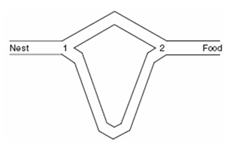
\includegraphics[width=0.5\textwidth]{Images/chapter1/doublebridge}
\caption[Double Bridge Experiment]{Image representing the Double Bridge Experiment. Image source \cite{doublebridges:image}}
\label{fig:doublebridge}
\end{figure}

\noindent
Figure \ref{fig:doublebridge} represents the scenario the Argentine ant were faced with for the Double Bridge Experiment. Initially there will be no pheromone trails for the ants to follow, so as the first ant approaches intersection marked \enquote{1} in figure \ref{fig:doublebridge} the probability that they choose the top path, or lower path is therefore $\approx$50\%. Regardless of which path the ant chose pheromone will now be deposited on the corresponding path. The next ant will approach the intersection marked \enquote{1} however, as there now exists a pheromone trail this ant now no longer has an equal probability to choose either path but instead is more likely to choose the same path as the previous ant. This process will continue for every ant in the colony. Generally speaking as the bottom path is significantly longer than the top path, the pheromone deposited on the lower path will ultimately have a lower pheromone concentration than the shorter top path. Overtime this will cause more and more ants to take the top path over the bottom path due to the higher pheromone level directly impacting the probability of the ant choosing this path. The same applies to intersection marked \enquote{2}, the ants will still tend to prefer the path with the greater pheromone concentration, the fact that the ant now has food does not affect the ants choice in anyway, aside from the fact that the ants new target is the nest and no longer the food source.

\section{Travelling Salesman Problem}
\label{tsp}
Ant Colony algorithms are commonly applied to the Travelling Salesman Problem (TSP). The TSP consists of a graph of $n$ cities and a path between these $n$ cities must be found however, each city must be visited exactly once. Generally this $n$ value is rather large for example the Berlin52\cite{berlin52:source} is a variation of the TSP where this $n$ value is 52. The number of possible routes between these 52 cities is incredibly large and exploring every combination is a near impossibility. The application of heuristic algorithms such as the Ant Colony methods enables solutions to be found within a reasonable time. One solution for the Berlin52.tsp problem is shown in figure \ref{fig:berlin52}.

\begin{figure}[h!]
\centering
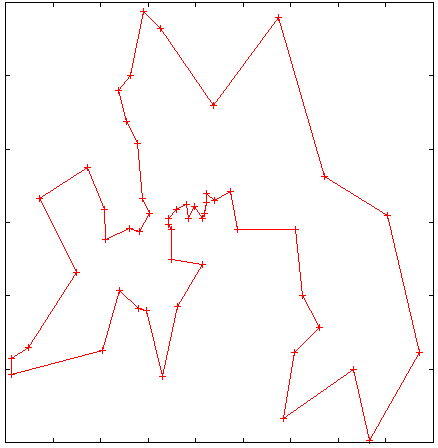
\includegraphics[scale=0.7]{Images/chapter1/tsp52}
\caption[Example Berlin52.tsp Solution]{One solution to the Berlin52.tsp problem plotted using GNU Plot. Modified version from original image source \cite{berlin52:image}}
\label{fig:berlin52}
\end{figure}

The TSP is not the only problem which can be tackled using the Ant Colony family of methods. As these methods have metaheuristic properties the general behaviours and structure can be applied to several other problems such as image segmentation however, this project will not cover such application and will focus on the TSP style of problem.

\section{Ant System}
\label{sec:AntSystem}
The Ant System is the most basic implementation of an Ant Colony Optimisation method, because of this it provides the basis for extensions and variations. Due to its basic nature, the Ant System is ideal for demonstrating and teaching the behaviours of a virtual ant colony to a user, and it can be done regardless of their prior background knowledge. In this implementation there is no recollection of the best path between iterations and every agent is equal in terms of its importance in finding a solution.

\subsection{Forumlae}

Sections \ref{ASprob} and \ref{ASphero} refer to the underlying formulae which govern the ants probablitity of selection and pheromone deposits for a given edge.

\subsubsection{Probability}

The probability formula is as described in appendix B, section \ref{sssec:probfuncsssec}. This is the function which drives the ants movement and enabled ants to generally pick the best looking path (path with the strongest pheromone concentration) whilst also allowing for ants to select other paths helping to prevent localised solutions forming.

\label{ASprob}

\subsubsection{pheromone}

The pheromone function for the Ant System algorithm is as described in appendix B, section \ref{sssec:pherodepo}. This function is the main difference between the Ant System implementation and the Elitist Ant System.

\label{ASphero}

\section{Elitist Ant System}
\label{eliteymcneaty}
The Elitist Ant System is the first adaptation to the initial Ant System algorithm. The Elitist Ant System is again, proposed by Marco Dorgio et al. in his 1992 PhD Thesis \cite{Dor1992:thesis}. The main difference between the Elitist Ant System and the Basic Ant System is the fact that the best ants for a given iteration have pheromone deposited upon their route. This means that the best $x$ number of ants where $x$ is an integer representing the number of elite ants will have their routes remembered across iterations preserving their best routes knowledge. This generally improves performance of the population as a whole as the extra pheromone on these elite paths will increase the probability that any ant traverses an elite edge (an edge that is part of a best routes).

\subsection{Forumlae}

Sections \ref{EASprob} and \ref{EASphero} refer to the underlying formulae which govern the ants probablitity of selection and pheromone deposits for a given edge.

\subsubsection{Probability}
\label{EASprob}

The probability function for the Elitist Ant System remains the same as it is in the Basic Ant System, see section \ref{ASprob} and appendix B, section \ref{sssec:pherodepo}

\subsubsection{pheromone}
\label{EASphero}
The pheromone function used in the Elite Ant System must acknowledge that there is pheromone to be deposited along the current $x$ elite routes.

\begin{figure}[H]
\Large
\begin{equation}
p_{xy}^{k} = (1 - \rho)\tau_{xy}^{k} + \Delta\tau_{xy}^{k} + e\Delta\tau_{xy}^{best}
\end{equation}

\caption[Elitist Ant System Pheromone Function]{Algebraic model of the pheromone deposit function for the Elitist Ant System \cite{marcdorgio:book:EAS}}
\label{fig:EASpheromonefunc}

\end{figure}

The majority of the formula remains the same as defined in appendix B section \ref{sssec:pherodepo} however, there is the addition $e\Delta\tau_{xy}^{best}$. This is the part of the formula which is responsible for the pheromone deposit on current the retained best (elite) paths. $xy$ refers to the $x$ and $y$ coordinate for an edge in the best path this is where pheromone will be deposited. $best$ simply donates that this edge belongs to one of the currently stored best paths. The $e$ value is a constant, and varies between implementations. Research suggests that a good value for this constant, $e$ is $\frac{1}{4}\ .\ \#\ of \ nodes$ \cite{sjored:Thesus2012:evalue} however, there is evidence to support using $\#\ of \ nodes$ as the $e$ value\cite{marcdorgio:book:nopage}.

\section{Existing Solutions}
\label{existingsolutions}
There are a number of pre-existing solutions which attempt visualise Ant Colony algorithms however, the majority of these based upon the authors experience are in fact sub-par in performance. Rather that visualising the algorithms execution in a logical manner, more often than not the existing solutions simply shows the algorithms final state without any detailed intermittent steps. This leaves the user confused about what has just actually happened and how was such a solution obtained.

Another problem associated with existing solutions is that the graphical user interface is too cluttered or complex. Many of the existing applications the author observed contained every interaction element in a tightly packed series of containers rather than splitting appropriate actions into separate views or menus. This is extremely confusing and makes it difficult to actually use the application as intended. If the user has selected that they want to use a specific variation of an Ant Colony algorithm then the user should only be able to interact with the features directly relevant to their selection.

One of the major problems the author faced when assessing the competition was the fact that there was rarely any visualisation of the agents themselves. As a result the user had to effectively guess which cities the agents were currently at. In addition to this there was no visualisation of the agent’s movement between city locations. This made it difficult to visualise the path the agents took aside from coming to your own conclusion based on the pheromone trails which were also often poorly represented.

\section{User Interaction Methods}
\label{uiMethods}
As discussed in section \ref{existingsolutions} the methods of user interaction must be superior to what is provided by the competition. This application will be authored in accordance with several preferred user interaction methods enabling a more user friendly experience for all users and not just those who are experienced with this or similar applications.

\subsection{Law of Context}

The law of context refers to the users expectation that they should only see interface controls relevant to the current object they want to modify \cite{99designs:laws}. This relates to one of the fundamental problems found in competitor applications (see section \ref{existingsolutions}). Should the user request a change of algorithm type which requires an extension to default features, these new controls will be self-contained and represented suitably so the user knows that the new dialogues or interaction methods are a direct result of a change in algorithm type.

\subsection{Law of Feedback}

The law of feedback relates the ideology that every significant action has some form of informative, relative feedback associated with it\cite{99designs:laws}. This enables the users to quickly develop an understanding of which interaction controls which action. The application will be developed in such a way that any incorrect actions will be displayed to the user in a manner that anyone can understand and provide the user with the required knowledge to resolve said issue.

\subsection{Law of Easing}

The law of easing is very important, especially for this application. This law suggests that complex actions should be segmented into simpler steps to allow the user to comprehend what they are actually doing \cite{99designs:laws}. The way this application will adopt this is that rather than specifying all of the algorithm’s parameters at once, each parameter will have its own method of interaction and its own series of user feedback prompts enabling any user to simply modify select parameters however they see fit, assuming the value is legal.
%\addcontentsline{toc}{chapter}{Development Process}
\chapter{Design}

You should concentrate on the more important aspects of the design. It is essential that an overview is presented before going into detail. As well as describing the design adopted it must also explain what other designs were considered and why they were rejected.

The design should describe what you expected to do, and might also explain areas that you had to revise after some investigation.

Typically, for an object-oriented design, the discussion will focus on the choice of objects and classes and the allocation of methods to classes. The use made of reusable components should be described and their source referenced. Particularly important decisions concerning data structures usually affect the architecture of a system and so should be described here.

How much material you include on detailed design and implementation will depend very much on the nature of the project. It should not be padded out. Think about the significant aspects of your system. For example, describe the design of the user interface if it is a critical aspect of your system, or provide detail about methods and data structures that are not trivial. Do not spend time on long lists of trivial items and repetitive descriptions. If in doubt about what is appropriate, speak to your supervisor.
 
You should also identify any support tools that you used. You should discuss your choice of implementation tools - programming language, compilers, database management system, program development environment, etc.

Some example sub-sections may be as follows, but the specific sections are for you to define. 

\section{Overall Architecture}

\section{Some detailed design}

\subsection{Even more detail}

\section{User Interface}

\section{Other relevant sections}
\chapter{Implementation}

The implementation should look at any issues you encountered as you tried to implement your design. During the work, you might have found that elements of your design were unnecessary or overly complex; perhaps third party libraries were available that simplified some of the functions that you intended to implement. If things were easier in some areas, then how did you adapt your project to take account of your findings?

It is more likely that things were more complex than you first thought. In particular, were there any problems or difficulties that you found during implementation that you had to address? Did such problems simply delay you or were they more significant? 

You can conclude this section by reviewing the end of the implementation stage against the planned requirements. 
\chapter{Design}
\label{DesignSec}
This chapter describes the design rationale for the current system. This chapter will cover the overall system architecture, user interface designs as well pseudo code representations of the main, non-trivial algorithms. Chapter \ref{processSec} states how the author has a somewhat flexible approach enabling adaptations to the initial design. The proposed design in appendix B, and the final structure of the system are very different.

\section{Language}

The author has identified that the choice of language is an essential decision which must be made early in the projects development. Appendix B, section \ref{lang} denotes the language decision process the author went through.

The use of an appropriate language became even more important due to the fact that the design has undergone significant modifications since the initial proposal. If the author had selected a language which he had little experience with then the changes made to the initial design may have been much more complicated to implement. The author is very familiar with Java, more specifically Java 7 (Java 1.7) and above thus, implementing new features or refactoring existing code is familiar territory. The initial language choice (appendix B, section \ref{lang}) did not factor in the potential for radical design change however, if it did the outcome would not change and the existing rationale would still be applicable to the project. In the authors opinion Java is the most appropriate language for this project.

\section{Development Tools}
\subsection{Development Enviroment}

\subsubsection{Command-line Tools}
\label{sseccmd}
The author considered using a simple text editor such as Atom\cite{atom:textEditor} to write the code, and the command-line to compile said code using the default Java complier. Atom is a free, open source hackable text editor provided by GitHub and provides syntax highlighting support for numerous language including Java. This syntax highlighting is especially useful and makes the writing of the source code slightly easier, as is becomes much simpler to track the start and termination of specific code blocks. However, as Atom does not have built in Java compilation abilities, the compilation process can become complicated.

The problem with the above method of compilation is that error detection and correction can become a very tedious process. If any complication errors are present the trace presented in the terminal window can sometimes be quite difficult to parse resulting in increased difficulties tracking down the errors source. For smaller projects, this method of complication is perfectly suitable and can be effectively managed. This project as discussed in section \ref{processSec} is a rather large project for the author to undertake. As a result, the combination of source code size and manual compilation leads the author to believe this method of writing and compiling code is not only inefficient, but also inappropriate for this project.

\subsubsection{Integrated Development Environment}

The use of an Integrated Development Environment (IDE) can help to alleviate the problems that can come from using a writing and complication process such as that defined in section \ref{sseccmd}. There are many IDE's which support Java, however the author's preference is the use of the Eclipse IDE for Java Developers \cite{eclipse:IDE}. The Eclipse IDE provides a multitude of useful features as part of their default package. 

One of the main features which Eclipse provides is automatic building of the projects source. This is a major benefit when developing as you can simply write your code and run the built project without having the unnecessary complication of switching between several applications to achieve the same task. Also, as there is automatic building, any compilation errors will be clearly highlighted using a system which is familiar to most computer users. If there are any miss-spellings of method or variables names for example, Eclipse will underline these in red to show there is a clear problem with this exact line of code. This is similar to the default scheme provided by most word processors, enabling a logical mapping between this red underlined line of code and an errors presence.

Another useful feature provided by the Eclipse IDE is the auto completion of variables and method names. This has sped up the development process for the author as there was no need to constantly look at the API's or other project source files for method names, the author could simply type the object of interests identifier and see a list of all methods and variables associated with such object. This is easily done if the author used an approach similar to that discussed in section \ref{sseccmd}.

In addition to the built in compilation feature, Eclipse also provides an integrated debugging toolkit. The Eclipse debugger enables easy break point management, as well as all the usual features you would expect from a debugger such as; step through, step over and exploration of objects and variables. These features are also provided by command-line debugging tools however, the author is far more comfortable using a graphical interface to debug the application as it is easier to access the features of the debugger.

Eclipse also has built in Junit support. This project will use the JUnit library as part of the testing process (more details see \ref{junitsupport}). Similar to how the IDE makes the writing of the applications code easier, the support of test suites such as JUnit makes the test process much easier. The code responsible for the tests will also have access to the features provided by the IDE as mentioned above. In addition to this you can run the tests inside the IDE and get accurate feedback on how many test executed and how many failed and why these tests failed.

\subsection{Support Tools}

\subsubsection{Maven}

Maven is tool used for building and managing projects, specifically Java-based projects \cite{maven:site}. The Maven framework provides a lot of useful utilities for developing successful projects and ensuring that such projects adhere to certain standards. The Maven framework aims to provide convention, over configuration. If there are multiple projects which have many different dependencies, for example external Jar files, then Maven can allow other projects to make use of these dependencies. As the author is working alone and is not expecting to have any other projects which will share dependencies with this one, the author has to weigh up if this framework would actually benefit the development process.

Maven provides some useful testing capabilities. When testing using the Maven framework, tests are still written using the Junit libraries (see \ref{junitsupport}). The Maven framework provides some additional features which the author feels could be of use. Maven, will give the author a Unit test report should one be required which will cover numerous details, most importantly a test coverage report will be produced. This enables the author to assess how well the unit testing has been done. Although this test report is a very useful feature, the Maven framework is not a necessity nor is it complication free.

The main complication that the author has with use the of Maven for this project is that fact that as this is generally a small project, Maven and its features would not be fully utilised but the hassle of configuring the framework would still be present. The initial project configuration would be time consuming, given that the author is inexperienced with the framework and this time could be spent on the actual project development. There are plugins which enable Maven to be used with an IDE such as Eclipse, the author feels that Maven would not be appropriate for use here however, the test reports would be extremely useful.

\subsection{GitHub}

The author has seen the use of GitHub as an essential part of the development process. GitHub has enabled the author have strict version control throughout the development process. As this is the case, the author has been able to store a local repository which will exist as the working directory for the applications development whilst also allowing a working copy with the most up-to-date fully working project code to be stored safely online using GitHub. At numerous times throughout the development lifecycle the author had to revert back to a previous version of the applications code GitHub has allowed this process to be almost hassle free. As it is so simple to manage different versions of the application, each representing a different collection of working or non-working features the author has been able to develop in confidence as he knows that any mistakes or experiments are not as costly as there is always a backup version stored at the GitHub repository location.

Without the use of GitHub the author would have found it difficult to progress the application as expected. If there was no form of version control, then the mistakes the author made or external factors which then rendered the current development code unusable would be a far more disastrous. There was a time during development where the authors working directory became corrupt. This was easily resolved by simply retrieving the code stored in the projects GitHub repository. If GitHub was not being used here, there would the possibility that the author would have lost progress on the application.

\subsubsection{JUnit}
\label{junitsupport}

JUnit is an open source framework for unit testing Java applications. The Junit libraries provide a multitude of features that allow for a more simplistic approach to testing. Numerous other test frameworks are available however, the author is experienced with JUnit and feels that this framework is more than suitable for the unit testing of this application.

The author feels that a suitable testing framework is essential for efficient and accurate unit tests for any application. If the author had neglected to use a testing framework such as Junit and manually tested the application (looking manually for abnormal output (LMFAO)) then the quality and coverage of the unit testing would reduce significantly. If the author used a manual approach which relied on outputs then the author could potentially have a situation where the code is outputting the correct result but is internally flawed this cant be manually checked. This means that you could ship a product which is assumed to be functioning as expected then suddenly the application is misbehaving. A testing framework such as JUnit not only allows for the tests to be fully automated the tests also become scalable. Every code change would need to be re-evaluated against the existing unit tests, which is easily done if you have a series of test which can be executed automatically. If a manual approach was used, then it becomes a near impossibility that every change can be tested as it would simply be too much to check as the addition of this new code has scaled the number of application inputs and outputs as well the conditions in the codes logic.

\section{Overall Architecture}

The process used during this applications development has enabled the author to add additional features which were not additionally planned, this includes the addition of extra algorithm types and modifiers as well as refactoring of code into more logical methods and classes. The new application architecture is much more complex that the initial proposed design as a result each package will be represented as its own set of diagrams, then an overall representation showing the interactions between these packages will be explained. In all figures below, getter and setter methods are omitted but are assumed to be present. The packages referenced in this section will take the form of $che16.dcs.aber.ac.uk.xxx$ where $xxx$ is the corresponding package name.

\subsection{Controller}

The Controller package has undergone several changes since the initial design of the system as defined in appendix B, section \ref{sssec:cntrl}. The general ideologies have however remained the same the range of features provided by the application as a whole has increased thus, the author saw these modifications the Control package contents as a necessity in order correctly control these new features whilst also adhering to the existing Model-View-Controller framework.

\begin{figure}[H]
\centering
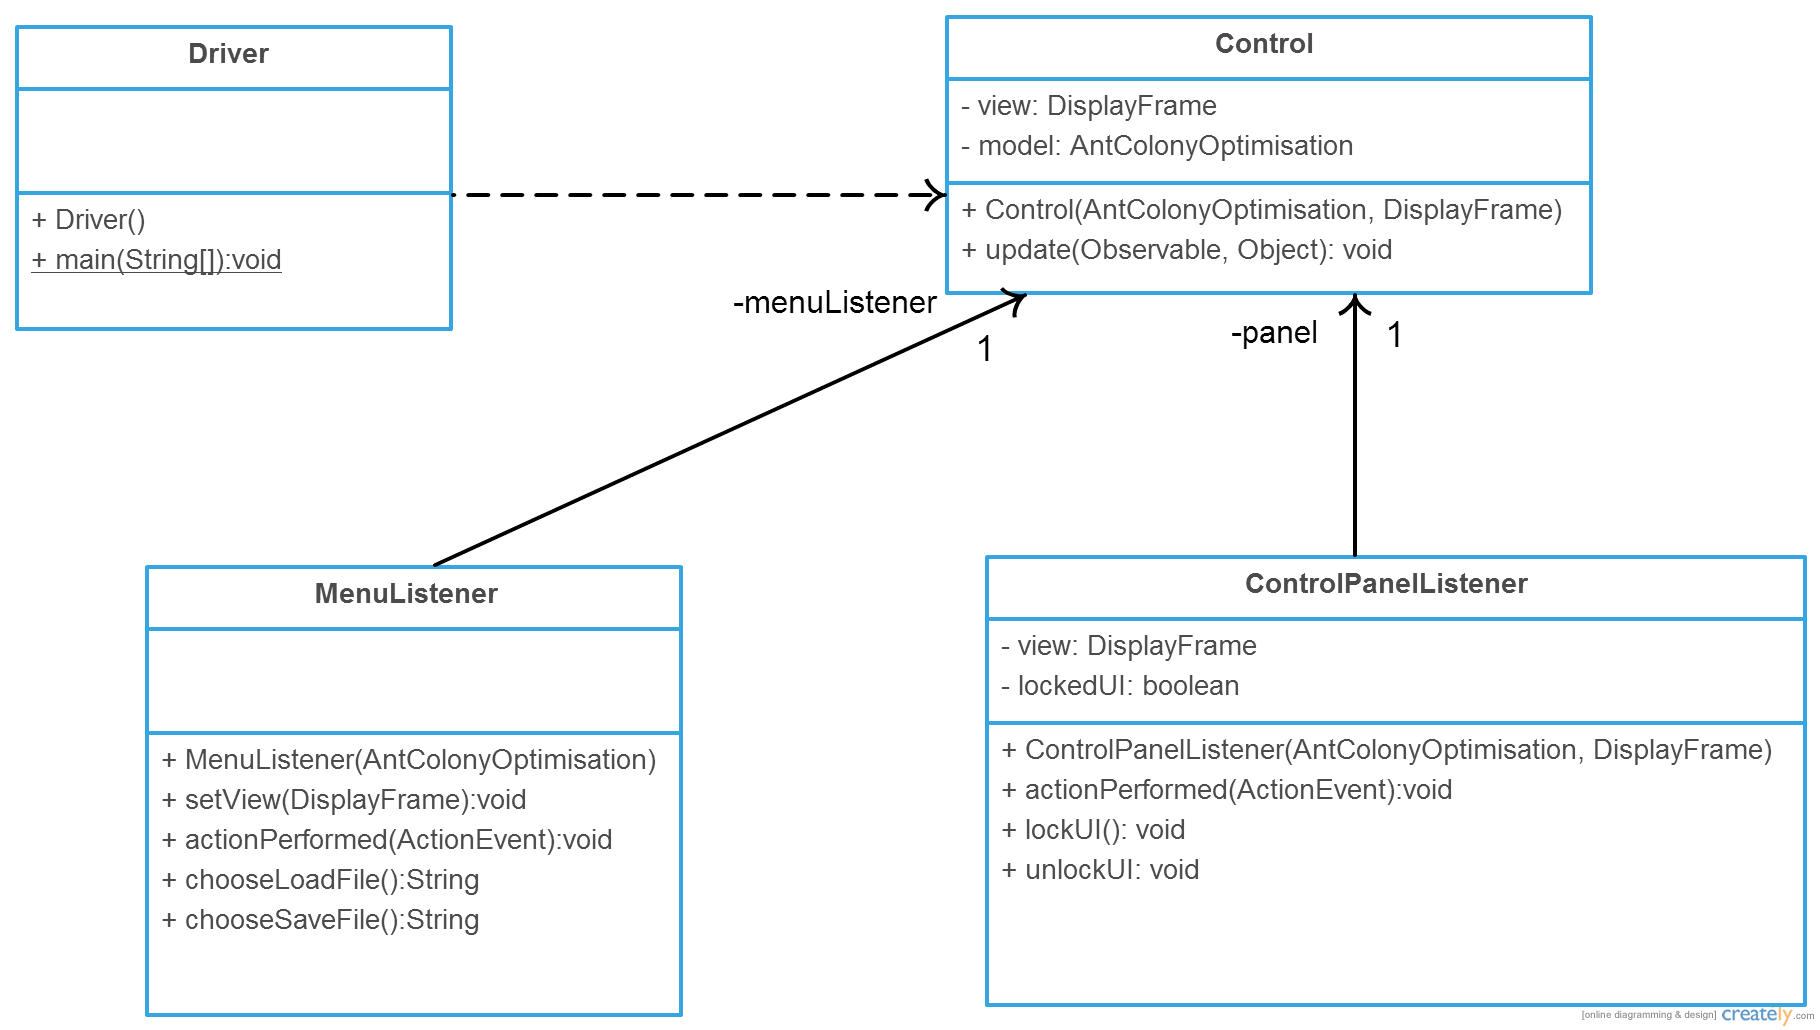
\includegraphics[scale=0.23]{Images/chapter4/controller}
\caption[Control Package Class Diagram]{The contents of the Controller package in standard UML Class diagram notation}
\label{fig:controllerImp}
\end{figure}

\subsubsection{Class Descriptions}

The Driver class remains largely unchanged from its initial proposed design (see appendix B, section \ref{driver:classdef}) however, it now interacts with the other components in a slightly different manner. The Driver class remains the sole entry point for the application. The Driver now has the additional responsibilities of instantiating the Control instance. The general purpose of the Driver class is still to ensure the system components are correctly instantiated, and holds no references to any instances of any object.

The Control as represented in figure \ref{fig:observableImp} is designed to observe the model and notify the view should the state of the model change significantly. In addition to this, the required instanced of MenuListener and ControlPanelListener are instantiated in this class and a reference to this Control object is maintained the created instances of said objects. The Control class is an additional feature not present in the initial design and is a result of the refactoring process. This class has the potential to be extended to support several other observable objects should this functionality be needed by the author in the future.

An instance of the MenuListener is used to listen the JMenuBar. This is designed collectively manage the actions represented by the elements contained in the JMenuBar. The alternative approach is to give each element in the JMenuBar its own Action Listener. This is far from efficient and increases both the codes complexity, and reduces overall maintainability of the application. The author decided to use a dedicated object such as this to listen to the menu and perform appropriate actions. This class maintains an instance of the Control class this enables the instance of this class to have access to the model and view instances stored in the Control instance enabling a simple way for the JMenuBar to have access to necessary functions.

A ControlPanelListener instance is designed to be a dedicated ActionListener for the ControlPanel (see section \ref{model:classdef}). Two separate ActionListeners are present in this application, this is because the author wanted to have dedicated listeners for each component, rather than having a combined object representing this class and the MenuListener. The author feels that this is appropriate as any modifications to the object which will be listened to becomes simpler to accomplish if relevant behaviours are extracted into logical modules such as this design exhibits.

\subsection{View}

The View package serves the same purpose as initial designed however, there has been a significant amount of refactoring applied to the initial design to enable a more effective graphical user interface to be created. The author has also added several new classes into this package to represent additional views which were not initially envisioned, but during development the author recognised that these new views were essential.

\clearpage
\begin{sidewaysfigure}
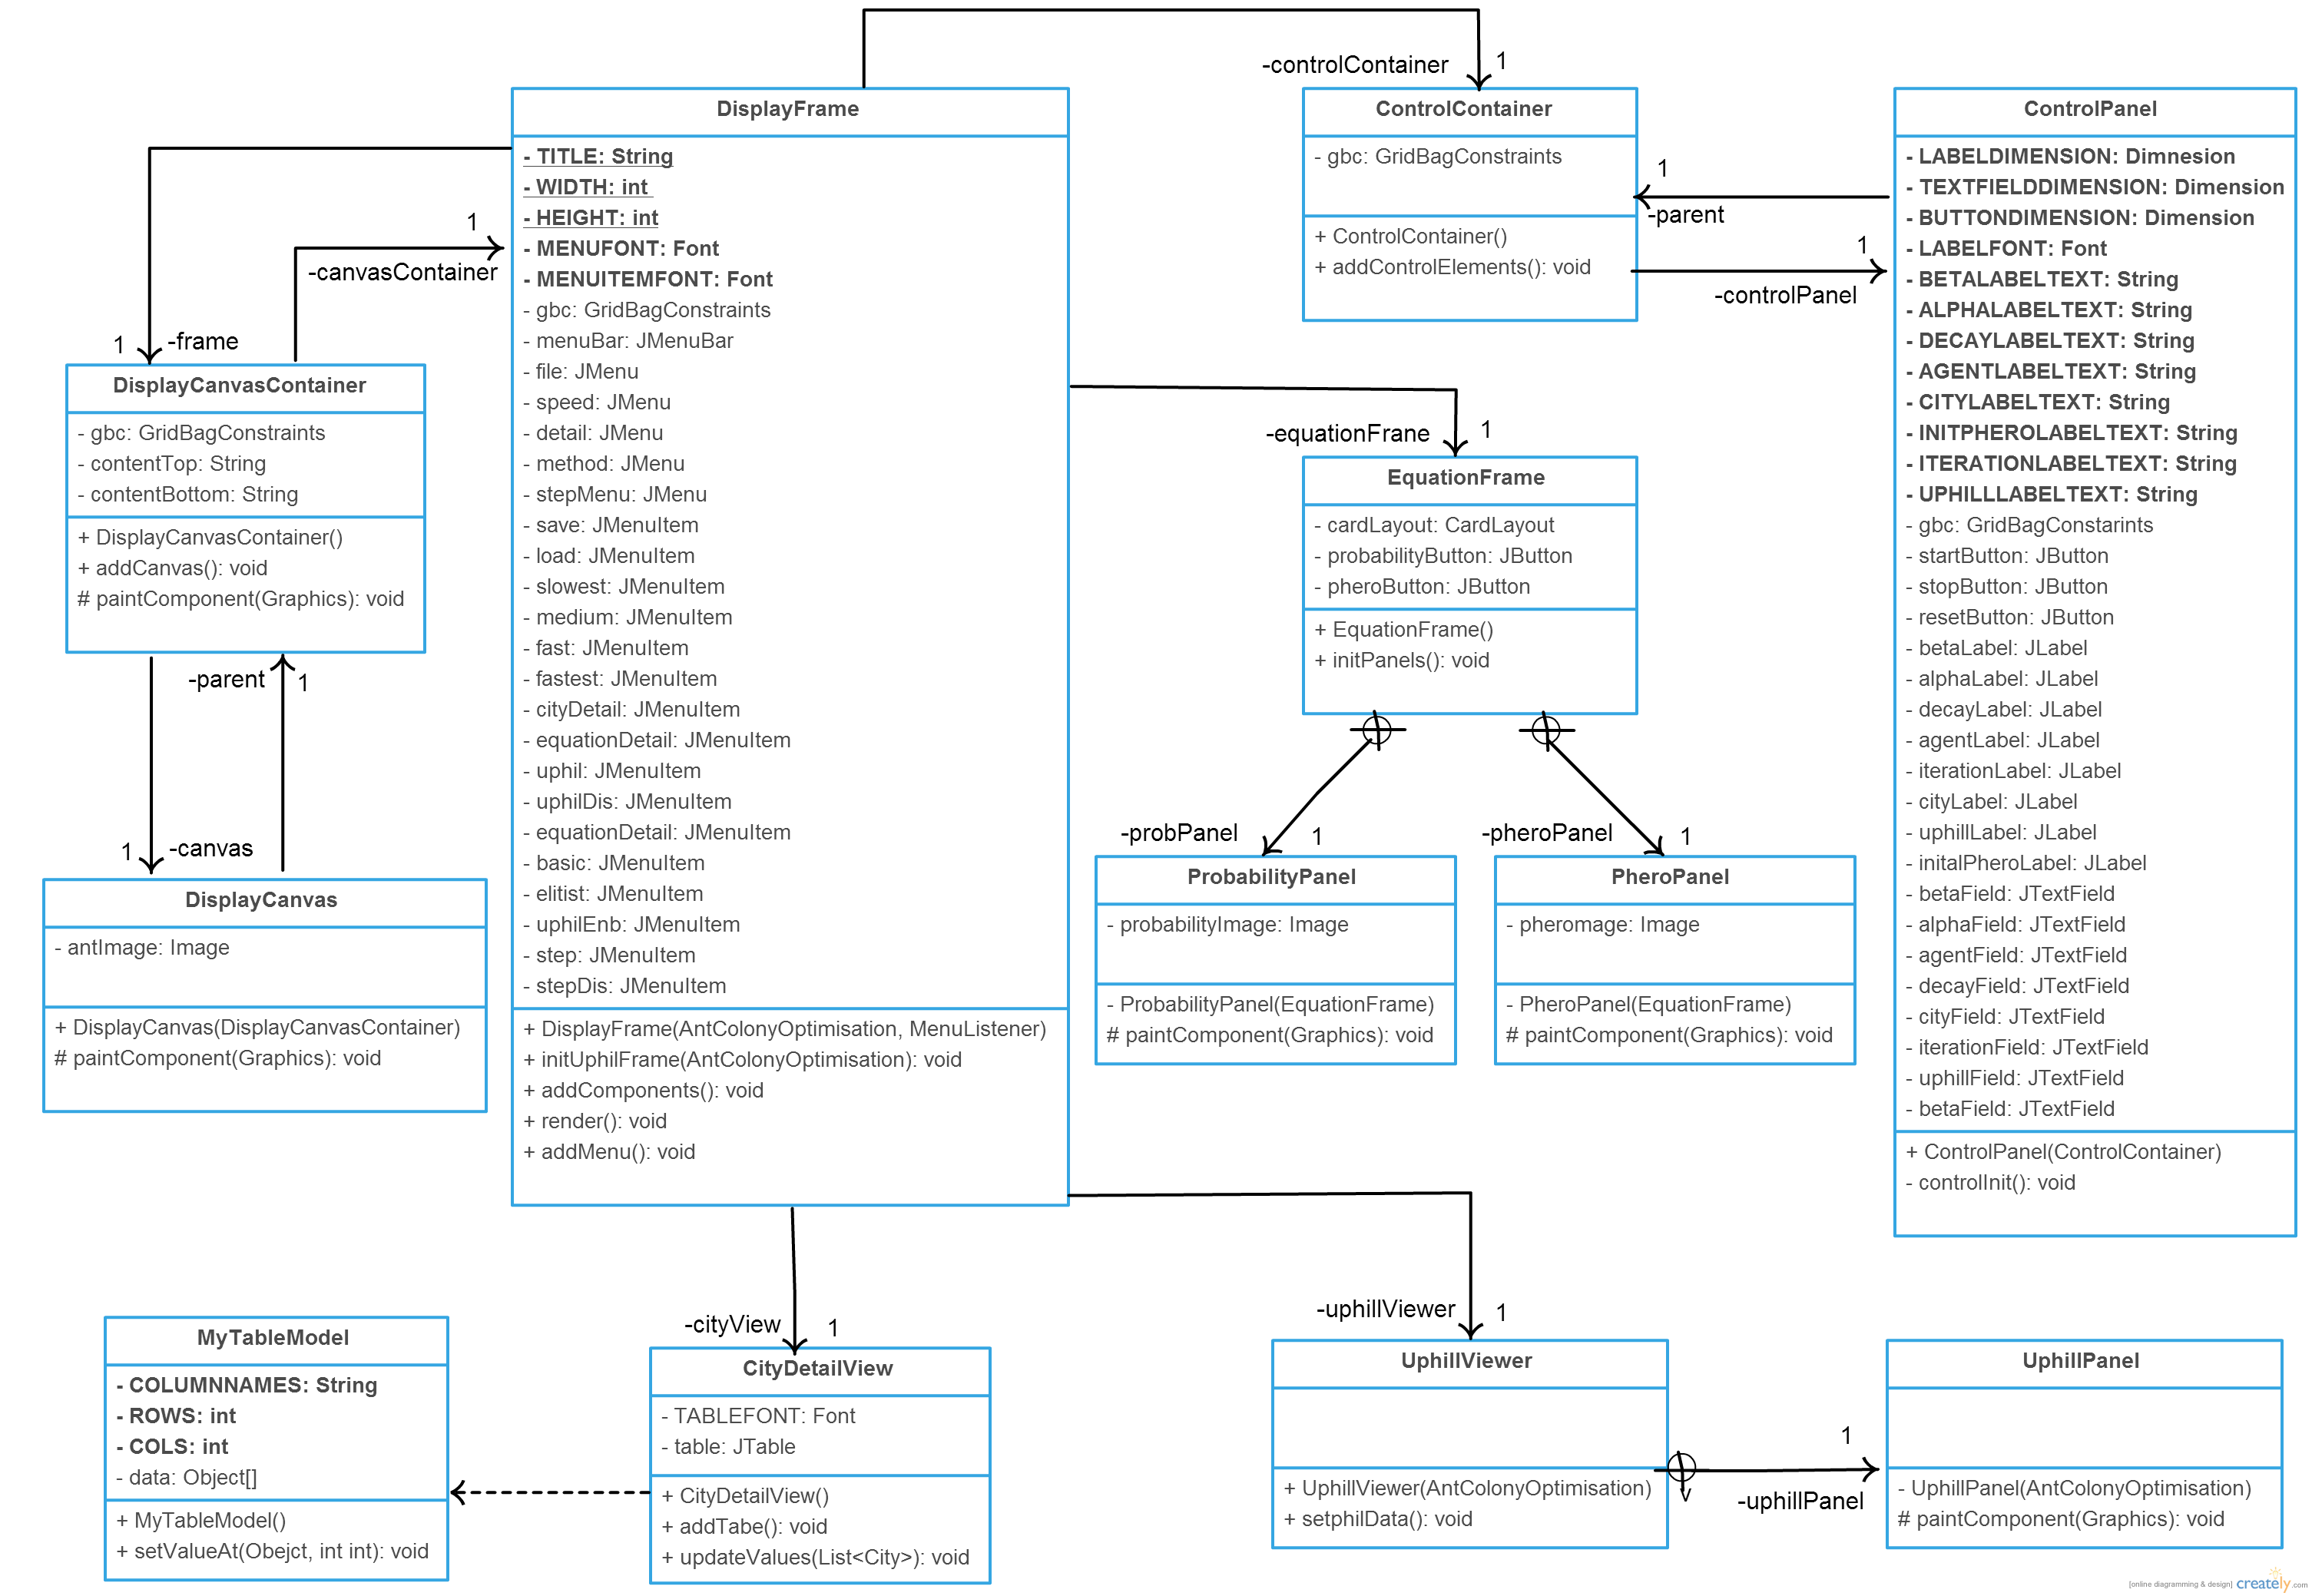
\includegraphics[scale=0.225]{Images/chapter4/view}
\caption[View Package Class Diagram]{The contents of the View package in standard UML Class diagram notation}
\label{fig:classdiagramImp}
\end{sidewaysfigure}
\clearpage

\subsubsection{Class Descriptions}
\label{view:clss}
Initially the DisplayFrame was designed to simply represent the highest level container which houses the remaining graphical user interface elements. As figure \ref{fig:classdiagram} shows the initial design for this class was very simplistic and lightweight. The author's decision to include additional user interface elements which were not originally planned has resulting in modification to the designed class. A JMenuBar has been added and as a result the DisplayFrame class grew in size in order to accommodate this JMenuBar and its necessary underlying elements. Although the size of this Class has grown the complexity and functionality is largely unchanged, it remains as the highest level container for the graphical user interface and control the instantiation of such elements.

The DisplayCanvasContainer is the result of renaming the DisplayPanel class in the initial design (figure \ref{fig:classdiagram}). This class is designed as a container to the DisplayCanvas instance, this functionality is as designed and the author has not modified its behaviour.

An instance of the DisplayCanvas class is used to visualise the algorithms state of execution to the users. This is the component that is painted during the algorithms execution using the $paintComponent$ method which it inherits from its JFrame super class. As the functionality provided by this Class is very simplistic, the current implementation remains unchanged from the initial design proposal (figure \ref{fig:classdiagram}).

The addition of the CityDetailView is a simple JFrame container which is used to display a JTable with data representing the number of agents currently at each city location. The JFrame displayed by this Class can be toggled between visible and invisible through user interaction with the respective JMenuBar item.

The structure of the table represented visually by the CityDetailView, is modelled by theMyTableModel class. Extracting the table’s structure into a separate class enables easy modification of the structure as well as reducing the coupling between the view and the table itself.

Similar to the DisplayCanvasContainer class, the ControlContainer is used to encapsulate the user input elements in their own separate container. This is a result of refactoring the UserInputPanel class in the initial design (figure \ref{fig:classdiagram}) into this container and the ControlPanel class. The main purpose for this class is to allow for a more diverse range of LayoutManagers to become available allowing for an easily modifiable interface.

The ControlPanel class used to contain the interface elements which directly relate to the creation and modification of the problem and world. This includes housing the text fields and labels required to enable the user to customise the algorithm parameters, as well as providing a simple means to start and stop the execution using a simple JButton approach. This class is essentially an extended version of the UserInputPanel class in the initial design (figure \ref{fig:classdiagram}) aside from the fact that more interface elements have been added the functionality is the same.

The EquationFrame class an extension of the JFrame Class which is used to display a graphic explaining the underlying algorithm functions. This class has no other functionality aside from the providing a means of displaying such graphics which is itself, contained within the ProbabilityPanel and PheroPanel Classes.

Both ProbabilityPanel and PheroPanel are nested classes inside the EquationFrame. These classes subclass JPanel and are used to contain different graphics which will be used to represent information relevant to the underlying probability and pheromone functions respectively.

The UphillViewer class is another new addition which was not perceived in the initial design. This class is a subclass of JFrame and is used to contain an UphillPanel instance. This JFrame can be togged between visible and invisible with relevant user interaction with the JMenuBar contained in the DisplayFrame.

An instance of the UphillPanel class is used to display information about the current status of the uphill routes for the current algorithms execution. This is an extension the JPanel class, enabling the uphill route data to be painted to the component using the inherited $paintComponent$ method. This is a nested class inside UphillView as no other objects uses or needs the knowledge of this a nested class is the most suitable way to contain it.

\subsection{Model}

The elements contained in the initial proposed designed represented in figure \ref{fig:classdiagram} has undergone significant refactoring which has produced a vastly different structure. During the development process the author found the the initial design happened to be inadequate for representing the algorithm in a suitable manner as it lacked necessary components and detail.

\clearpage
\begin{sidewaysfigure}
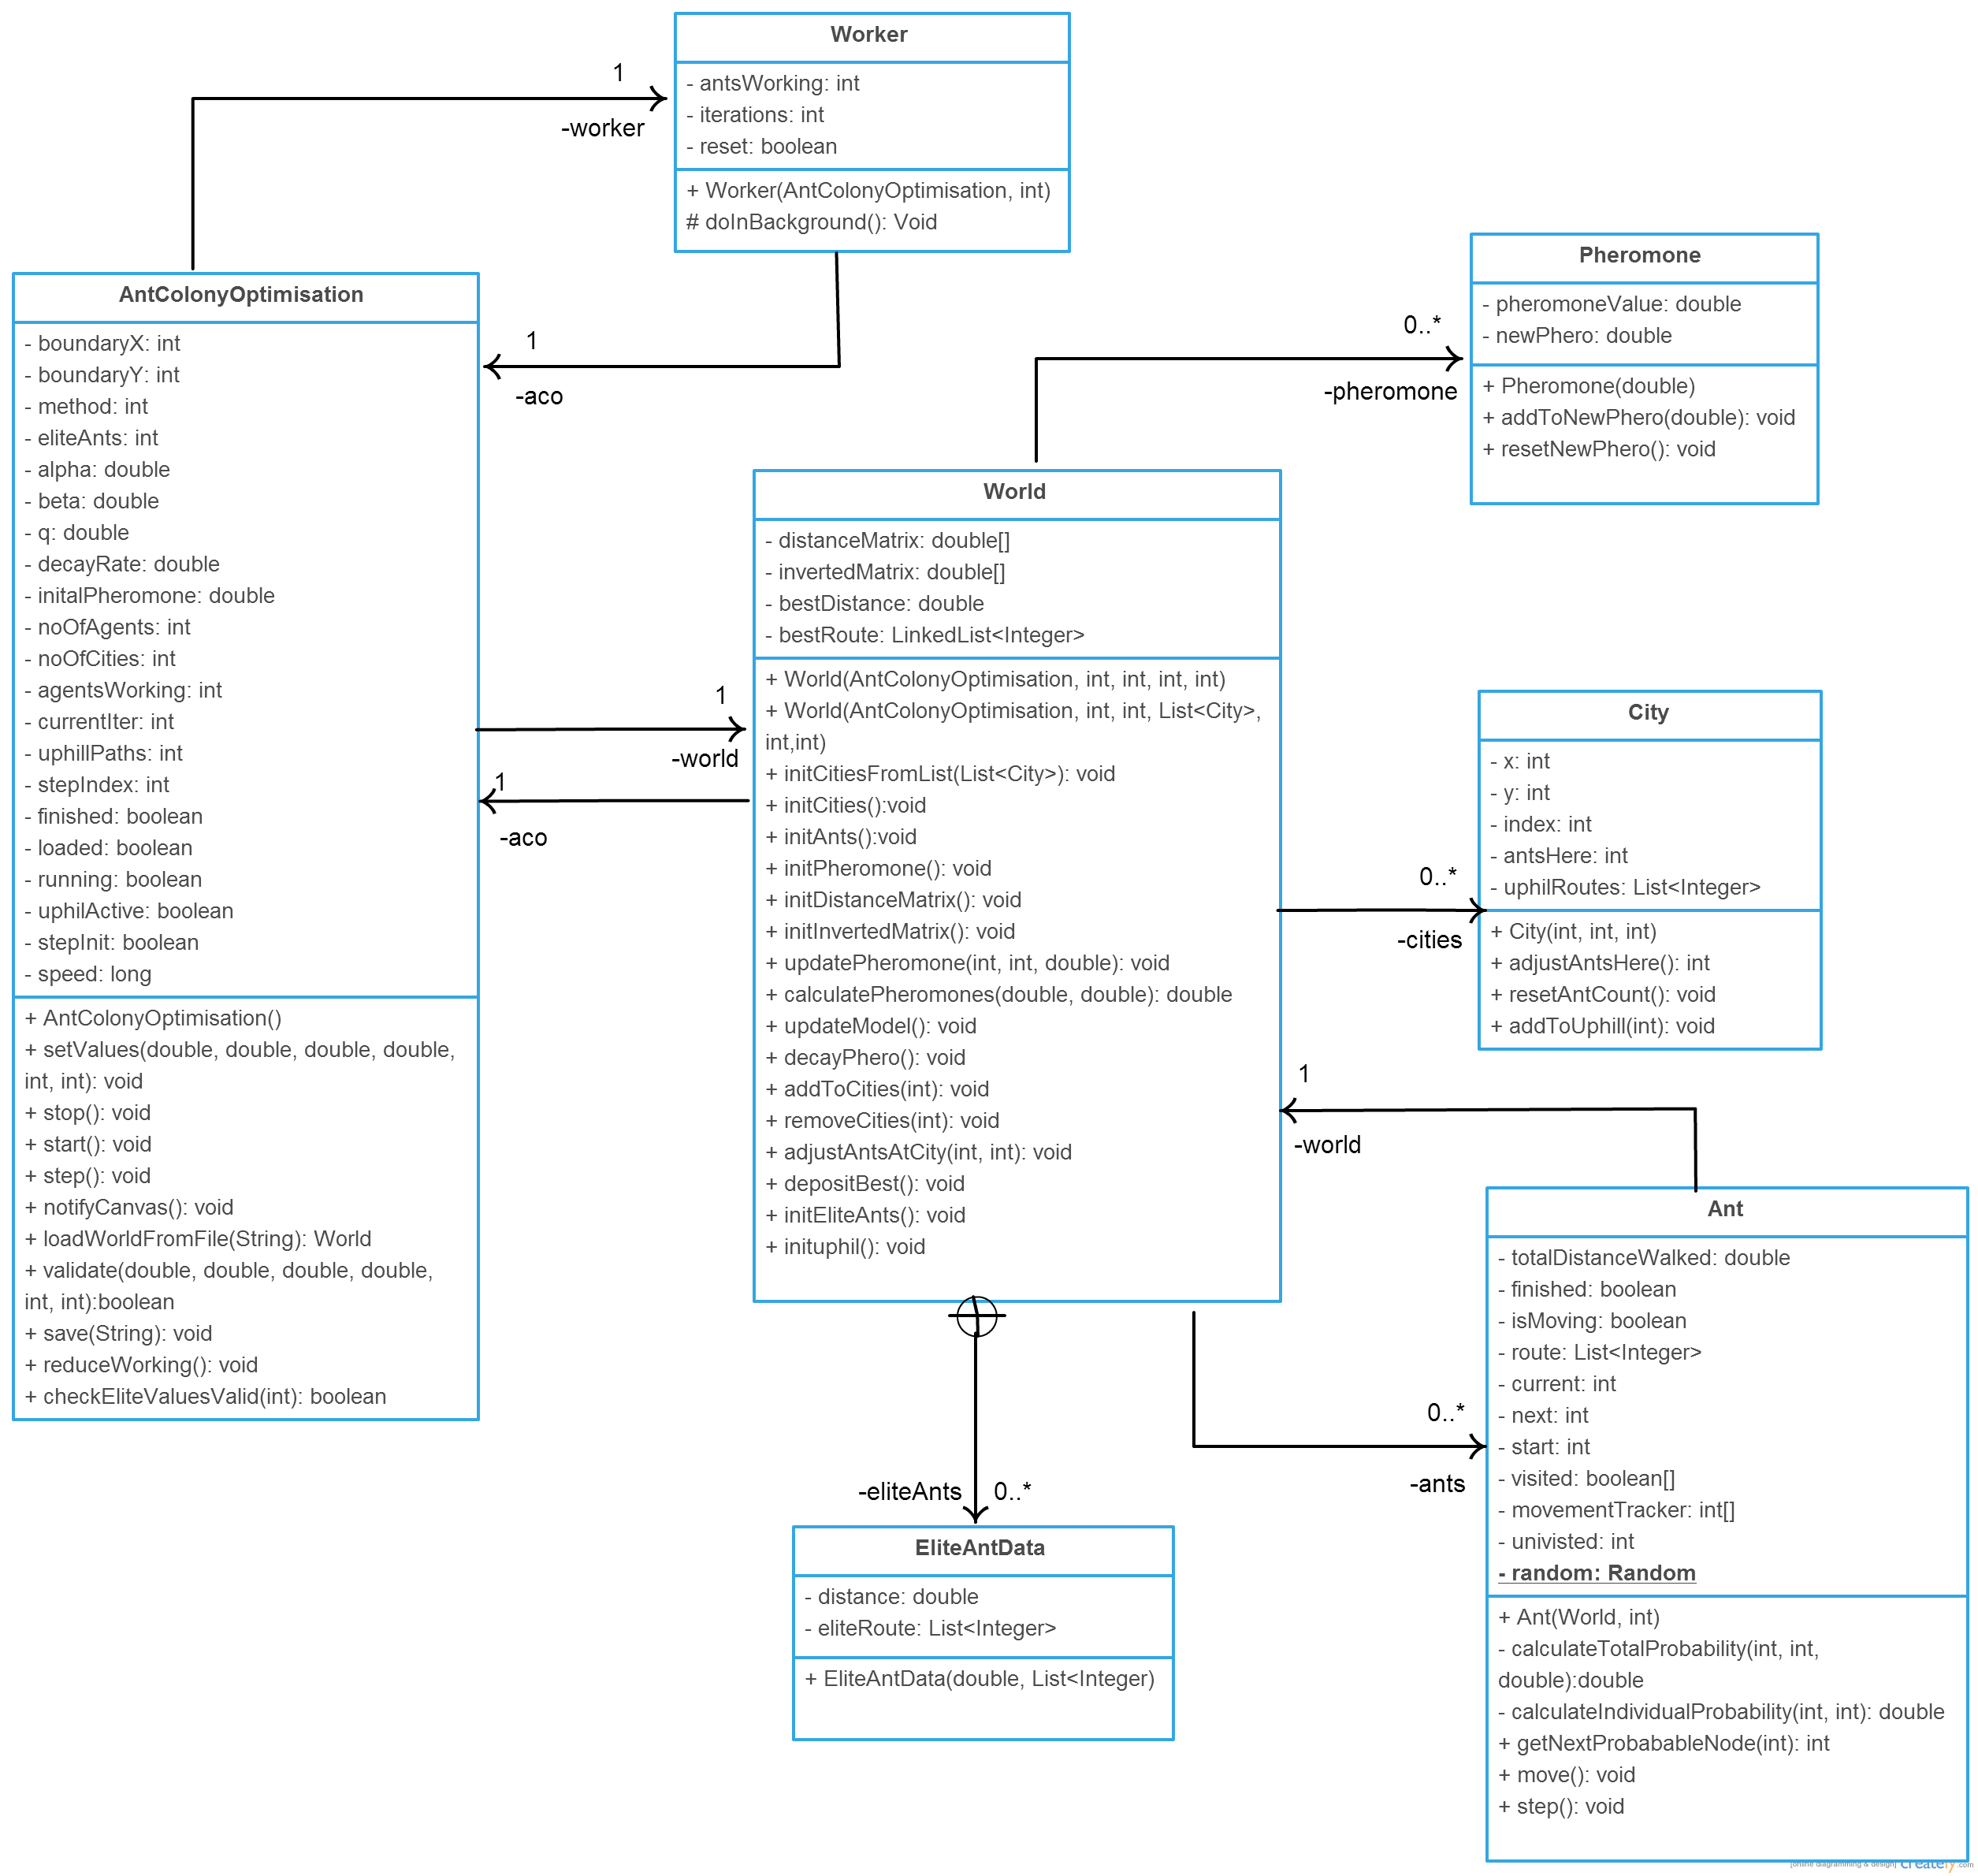
\includegraphics[scale=0.22]{Images/chapter4/model}
\caption[Model Package Class Diagram]{The contents of the Model package in standard UML Class diagram notation}
\label{fig:classdiagramImp}
\end{sidewaysfigure}
\clearpage

\subsubsection{Class Descriptions}
\label{model:classdef}

The initial concept behind the AntColonyOptimisation class is that this serves as the main control point and data centre for the algorithms execution. This class is used to store all the necessary parameter values and is also responsible for the instantiation of the Word representation. This class also controls external package access to the Model package and its data. This largely remains the same as designed however, there are slight modifications to accommodate additional functionality.

The Worker class was something that wasn’t initially planned. As discussed in \ref{swingmeupm8} there was a necessity for a way to control the algorithms execution without interfering with the performance of the interface. This class is an extension of the SwingWorker class and uses the inherited $doInBackground$ method to perform the algorithms execution in a suitable manner. 

The World class is used to model the problem representation and the environment for which the agents will be deployed during the algorithms execution. This class houses all the data relevant to such representations including a List of all Ant and City objects as well as having basic data structures which provide an effective representation of the pheromone concentrations for every edge within the graph and controls the manipulation of pheromones on such edges. This class is generally the same as proposed in figure \ref{fig:classdiagram} however slight modifications have been made to support additional features.

A City object is used to represent a node in the current problem representation graph. A collection of these City objects is maintained in the current World instance, and iterated through during both the solving and painting processes.

A Pheromone object is used to model the pheromone concentrations for any given edge. A two-dimensional array of these Objects is maintained in the current World instance, and these Objects are constantly manipulated during the pheromone deposit and decay operations. 

An Ant object is used to represent an agent which will be deployed in the current environment in order to solve the current problem. The World instance will maintain a collection of these objects. Each Ant has sufficient variables and methods to enable them to move and deposit pheromones accordingly. The initial design suggested the use of an AntInterface, however as the author has decided that there will only be one type of Ant thus, the interface is deemed to be unnecessary. Generally, this class is as designed in Figure \ref{fig:classdiagram}.

The EliteAntData is a nested class inside the World which is used to store the current elite routes. This feature is only necessary if the user has selected the Elitist Ant System as the current algorithm type. This is required to correctly preserver the best routes across iterations as the ant objects get reset each iteration. Rather than storing a whole ant object the author has opted only to store the best distances and best routes as this has less overheads when compared to storing an ant in full.

\subsection{Utils}

During development the noticed that some methods were being implemented in numerous locations. To prevent code duplication and promote re-usability the Utils package was implemented. This is a very simple package, containing one class however, the contents of this class don't belong in any other package individually.

\begin{figure}[H]
\centering
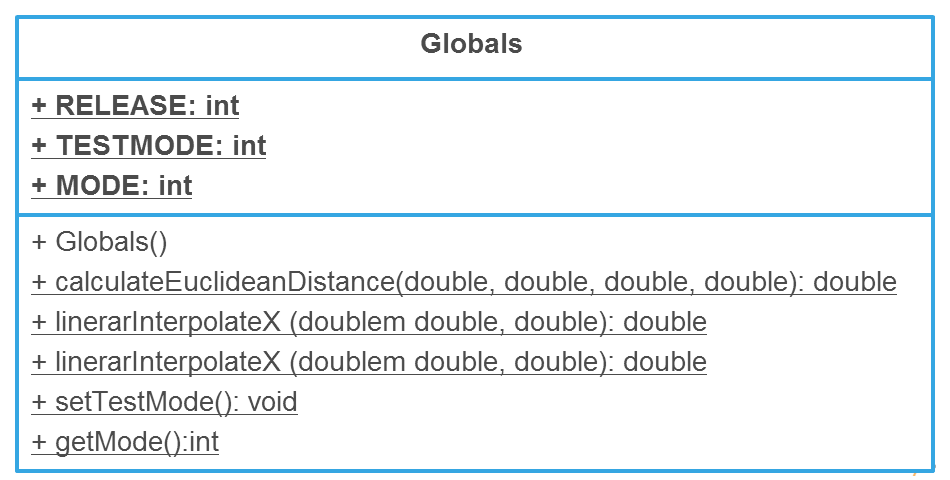
\includegraphics[scale=0.3]{Images/chapter4/gloabls}
\caption[Utils Package Class Diagram]{The contents of the Utils package in standard UML Class diagram notation}
\label{fig:utilsImp}
\end{figure}

Figure \ref{fig:utilsImp} represents the single class contents of the Utils package. This Globals class contains several publicly available static variables and methods enabling application wide access. This enables the multiple packages which rely on the results of such methods to retain access to them whilst also reducing the amount of repeated code. In addition this class enables the execution mode to be switched from release to test mode. When in test mode the error messages require no user response enabling the automated test process to complete more easily.

\subsection{System Interactions}

The different packages and their contents have been described above however, the interactions between packages must be carefully designed to ensure correct implementation and of the Model-View-Controller design pattern. 

\clearpage
\begin{sidewaysfigure}
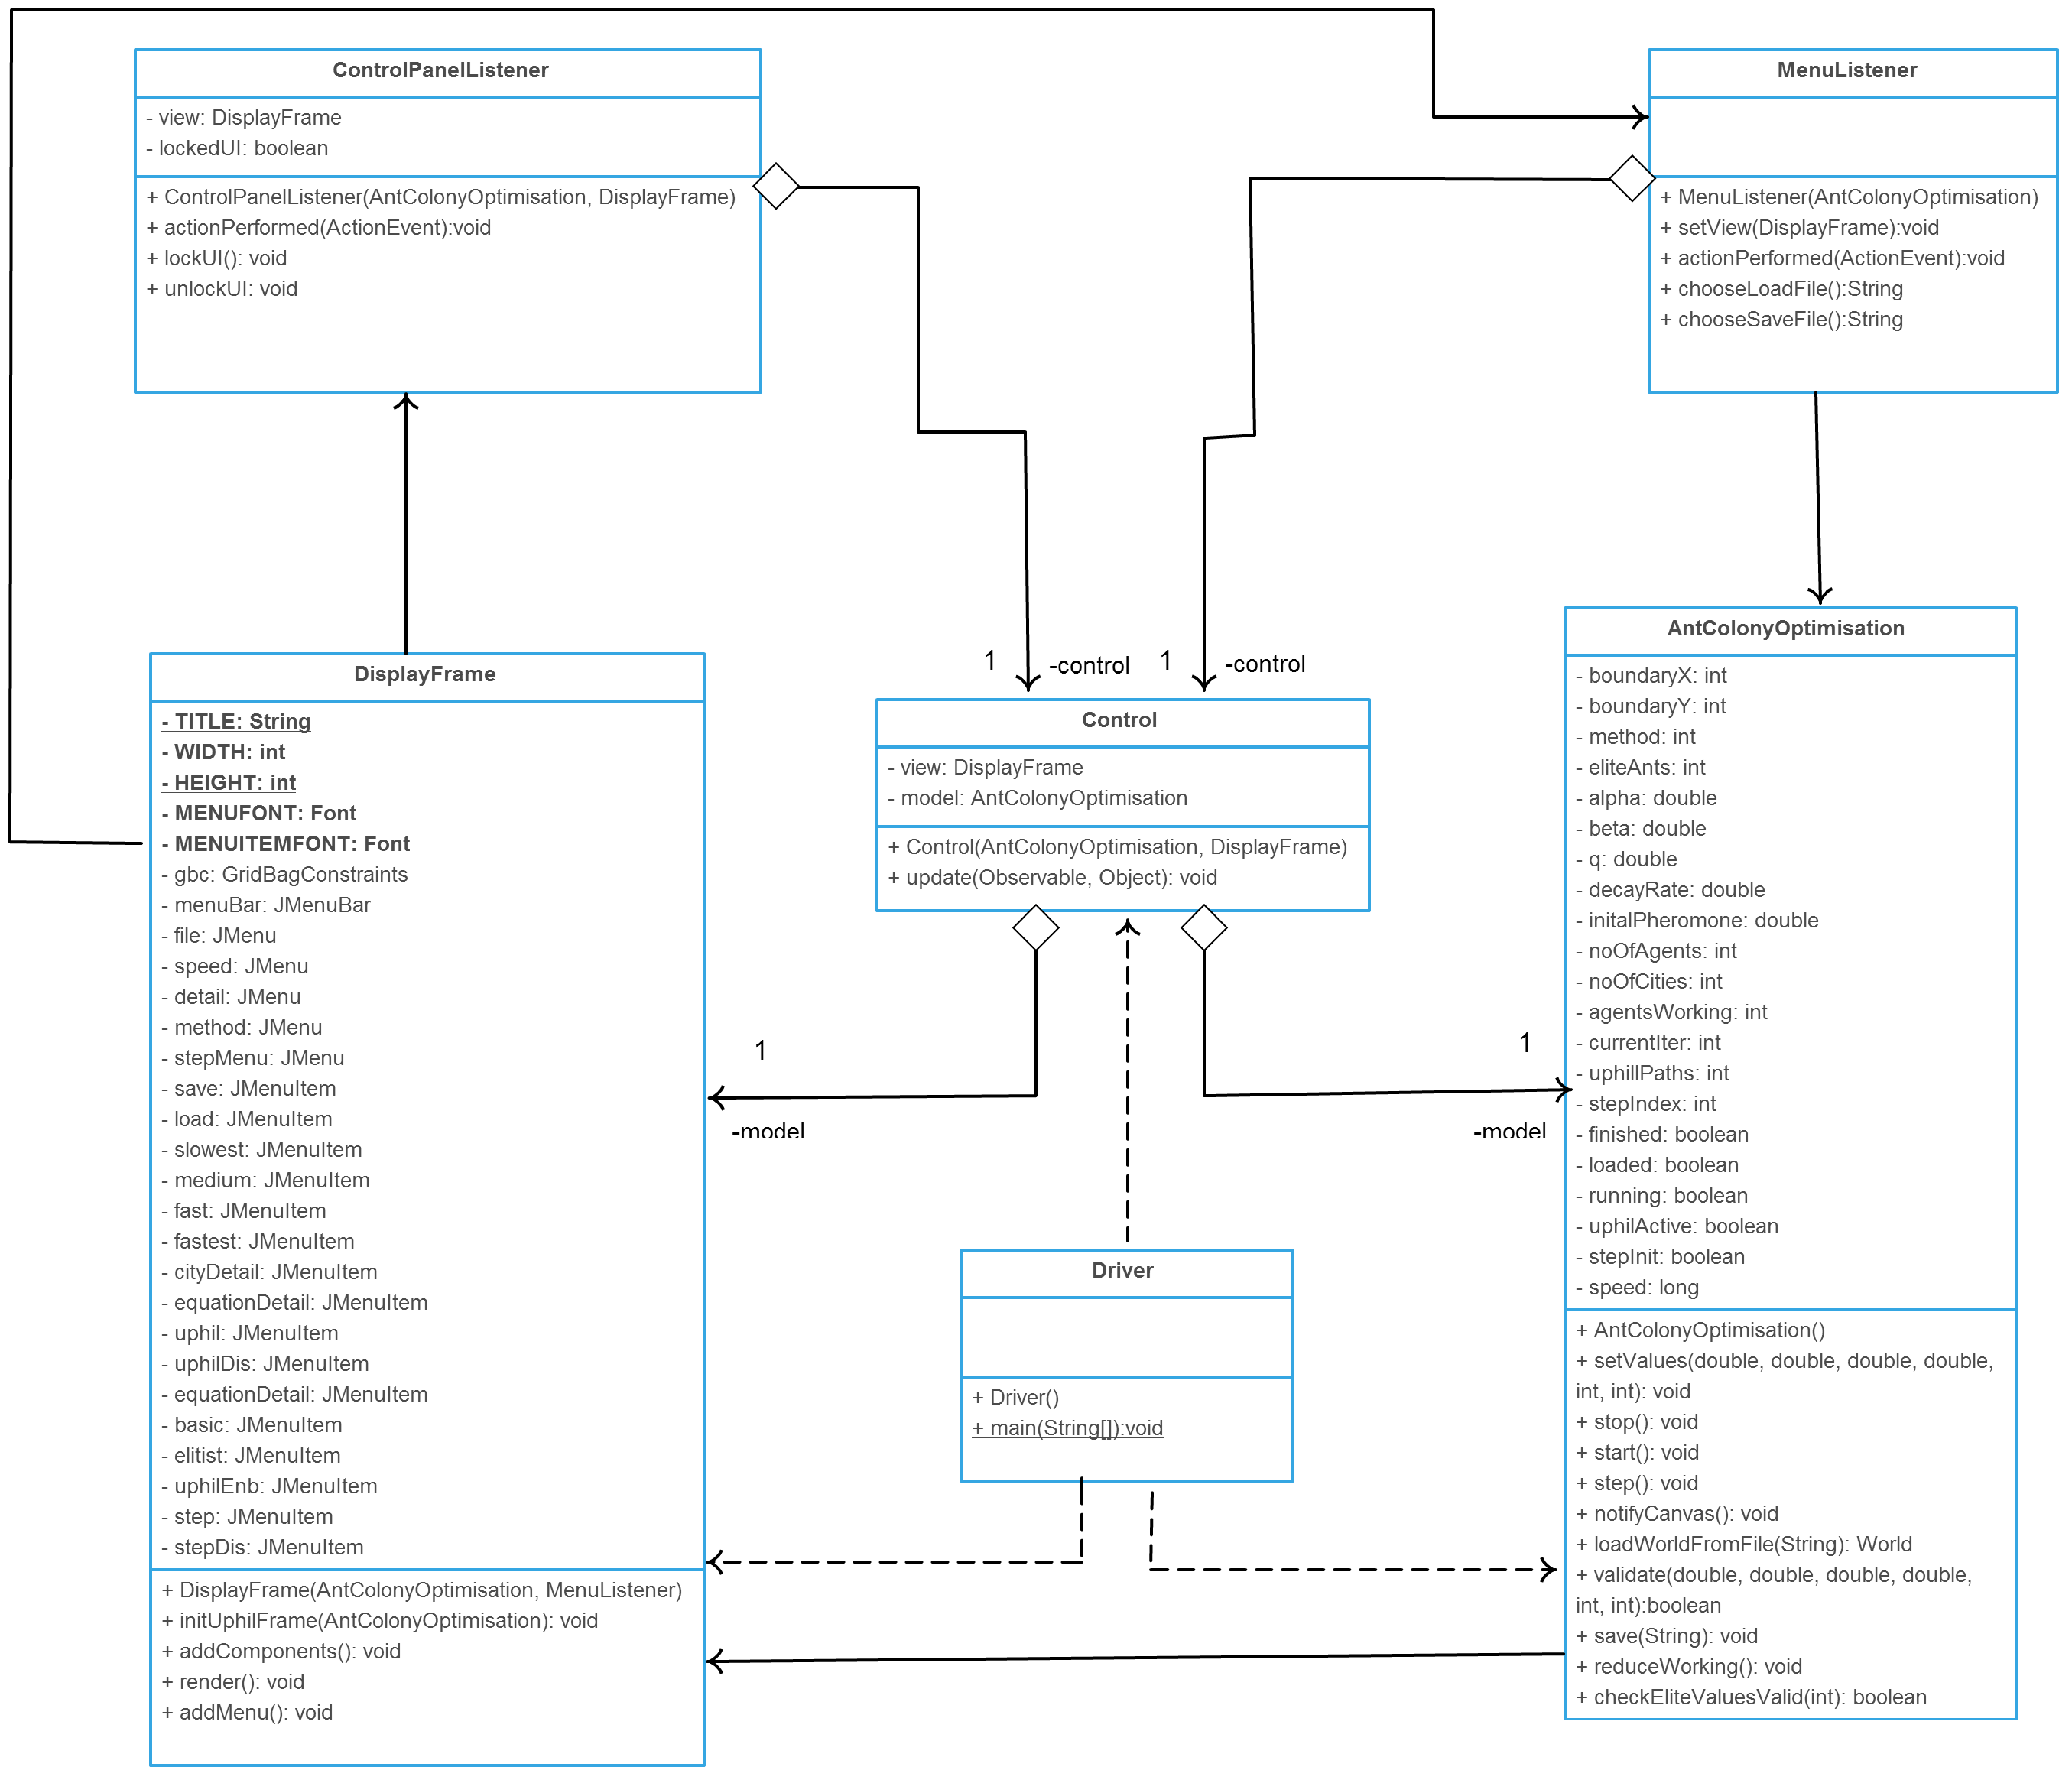
\includegraphics[scale=0.22]{Images/chapter4/overallClassinteraction}
\caption[Package Interaction Diagram]{The proposed manner of package interaction expressed in standard UML Class diagram notation.}
\label{fig:interacttion}
\end{sidewaysfigure}
\clearpage

Figure \ref{fig:interacttion} demonstrates how the access to the View and Model packages is governed by the instances of the DisplayFrame and AntConolonyOptimisation respectively. This keeps the interaction between packages simple and enables encapsulation of sensitive data. This design adheres to the Model-View-Controller principles as the Controller package and its contents govern the interactions between the Model and View. The view, has no reference to the model however, at runtime an instance of the AntConolonyOptimisation is passed to the View in order for the painting of necessary components to take place. As there is no explicit link between the model and view these packages can be easily modified or substituted in order to change the current representation there is no coupling between the contents of these packages.

\section{Design Patterns}
\subsection{Model-View-Controller}
The current design still adheres to the Model-View-Controller(MVC) principles discussed in Appendix B, section \ref{sssec:mvc} however, the complexity of the different package elements has increased. As designed, the author has implemented an MVC compliant architecture through the use of the Observer and Observable relationship using the corresponding default Java framework. The general concept is implemented as defined in appendix B, section \ref{obby} slight modifications have been made to the classes representing the different components of the Observer and Observable concept.

\begin{figure}[H]
\centering
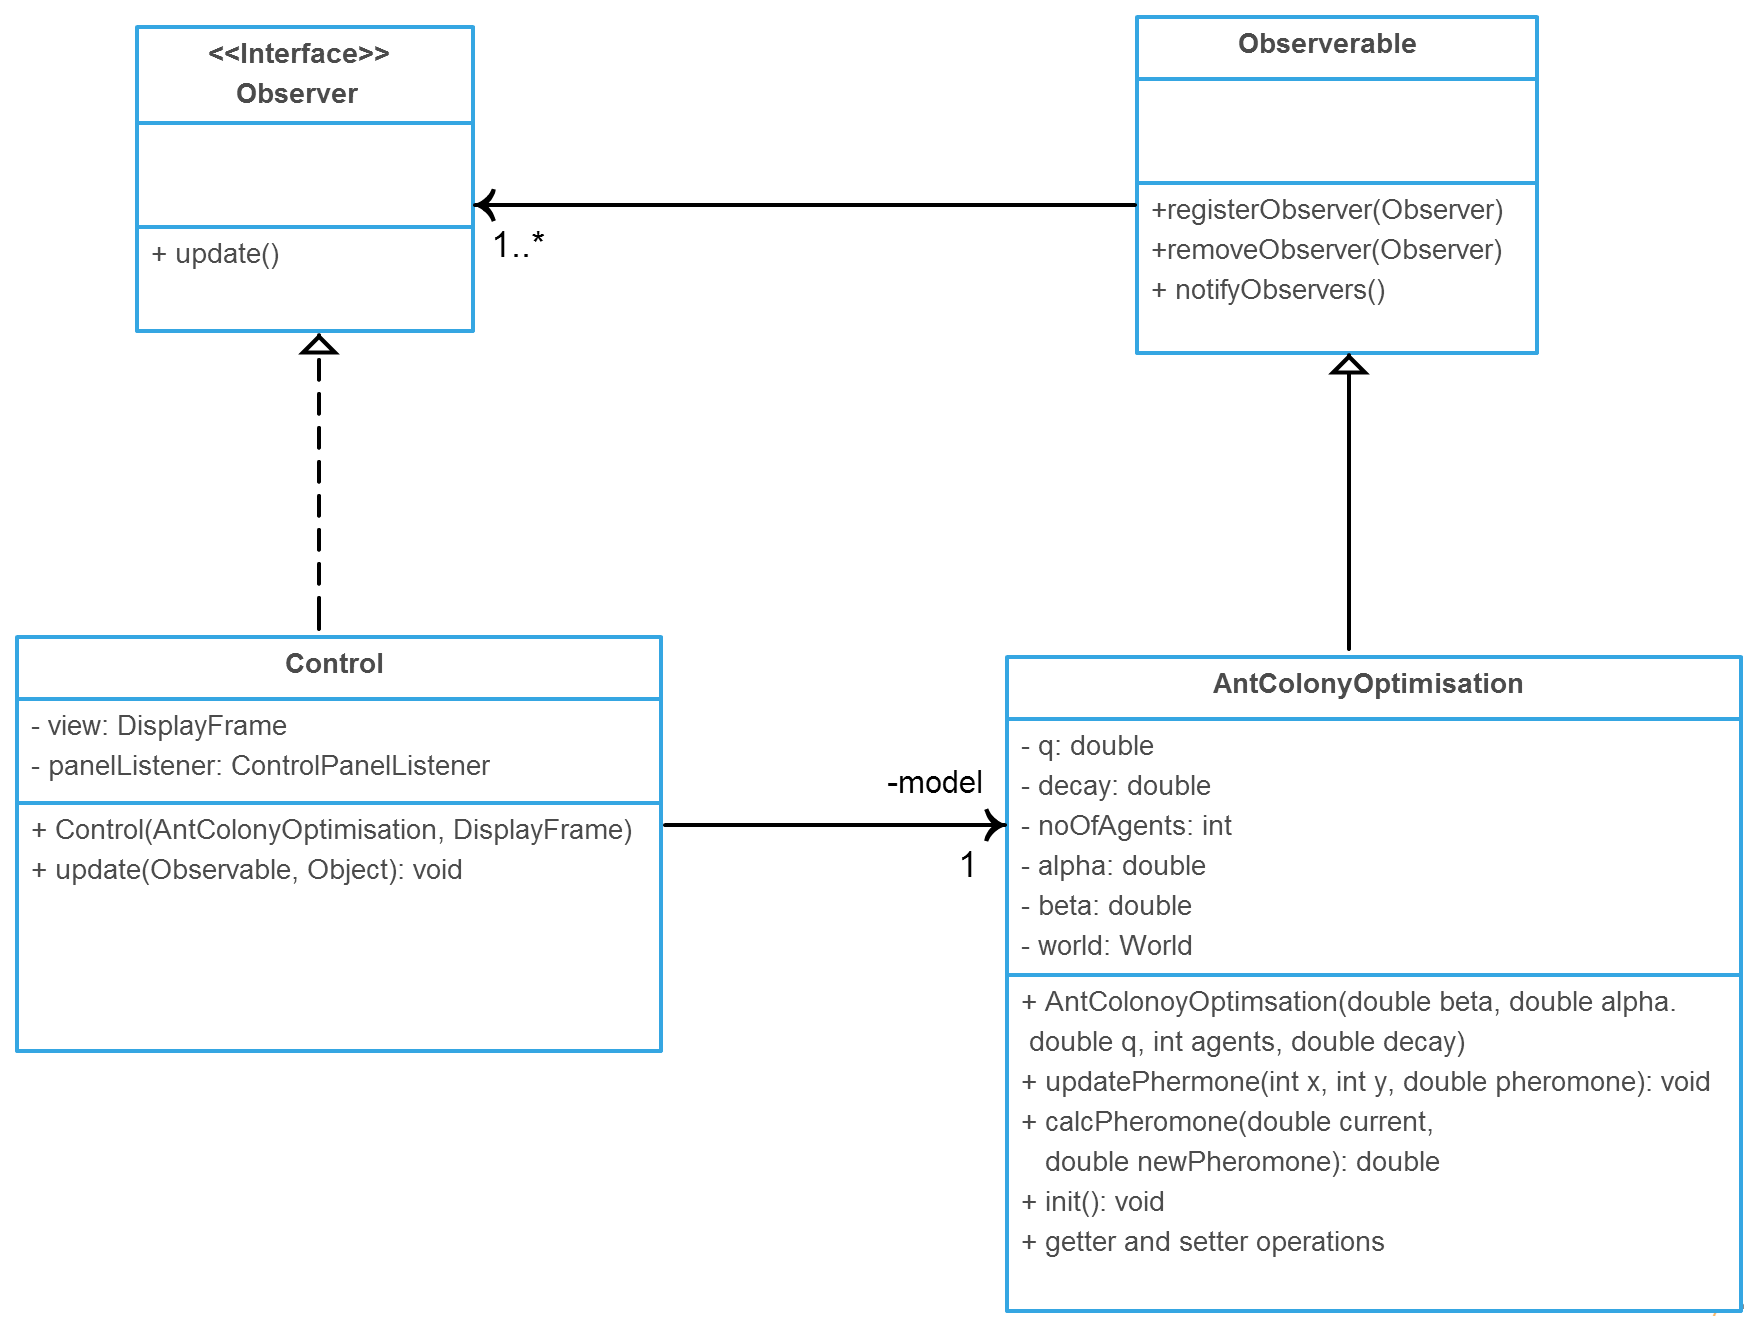
\includegraphics[width=0.9\textwidth]{Images/chapter4/observerImplemetation}
\caption[Observer and Observable Implementation]{Implementation of the Observer and Observable Design pattern}
\label{fig:observableImp}
\end{figure}

Figure \ref{fig:observableImp} demonstrates how the Control class will implement the Observer interface. This listens to the Observable object and determines the correct actions based upon the source of update. The AntColonyOptimisation class is as defined in section \ref{model:classdef} and acts as the observable object through its extension of the Observable super class. This inheritance grants the AntColonyOptimisation instance access to key methods such as $registerObserver()$ this allows the author to assign the Control instance as the designated observer. The $notifyOberservers()$ methods enables the author to dictate when updates are published to the Control instance which will the correctly update the View.

\subsection{Singleton}

Initially the author proposed that classes that compose the user interface would implement the Singleton design pattern\cite{gof:design:singleton}, an example this proposed design can be seen in appendix B, section \ref{sssec:singleton}. The author had initially implemented the interface witch each class implementing the Singleton pattern which caused complications. The Singleton pattern is however absent in the current architecture. As the instance of a Singleton object is globally accessible, difficulties arose during the application debugging. This issue happened to be more prevalent when extending the functionality provided by each of the Singleton classes, for example the DisplayFrame class now contains a wider range of functionality than initial planned. Not only did the Singleton instance complicate the addition of these extended features, debugging these features became more difficult as the global accessibility made it harder to track the source of the bug itself. This is due the fact that it is easy to accidently interact and modify a global variable or instance. Often the source of these bugs was not where the author expected and were often due to an incorrect interactions with these new extensions in a separate package. This was the main reason the author decided to withdraw the use of the Singleton pattern as the author felt it was much simpler to not have global access to these instances and features.

Robert Martin propositioned idea of the Single Responsibility Principle (SRP) in 1990 \cite{SRP:site}. The general concept behind the SRP is that each logical module in the software should have one reason to change or model one specific responsibility rather than a collection of unrelated features or functions. If a module has been extended to support multiple unrelated features, the SRP states that the unrelated features should be extracted into relevant modules so that each module maintains its one responsibility. The author feels that implementing the Singleton in the proposed manner (see appendix B, section \ref{sssec:singleton}) violated the underlying concepts of the SRP. As the Singleton class is responsible for tracking and instantiation of its one allowed instance and the functionality which the module presents, this class now has more than one responsibility and thus violates the SRP. The author believes the SRP should be regarded highly during development in order to produce maintainable and extendable software. As a result he has opted for adhering to the SRP over the Singleton implementations. The author experimented with the idea of having extracting the functionality of the Singleton classes and the tracking of the instance of such classes into separate system modules however, this vastly overcomplicated the architecture.

Overall, the author sees the implementation of the Singleton Design pattern as more of an anti-pattern. As this is the case and to enable easier modification the implementation of any Singleton class as initially designed has been removed. Solutions the above problems could be refactored in, but this is seen as unnecessary complexity by the author and has therefore also been omitted.

\section{User Interface}
\label{interfacebrah}
The user interface elements will be designed with the three laws of user interaction discussed in section \ref{uiMethods} as a top priority. The interfaces will be consistent in theme and styling which will provide application wide consistency for the user.

\subsection{Main Display}

The design for the main display, which refers the general view the user will be presented and interact with remains unchanged from the initial proposal as represented in figure \ref{fig:interface}. There has been modifications to this design during the implementation phase however, these the authors flexible process (see section \ref{processSec}) and the fact that these changes were fairly trivial allowed the author to implement them without any prior design, section \ref{mainimp} displays the implemention of this design and said changes.

\subsection{UphillViewer}
\label{uphillview}

The uphill viewer was not an element of the user interface which was initially planned, however the addition to implement the ability for a path to represent uphill terrain required a view to summarize which of these paths are in fact subject to this uphill modification. This interface is a result of the contents of the UphillViewer class (see section \ref{view:clss}).

\begin{figure}[H]
\centering
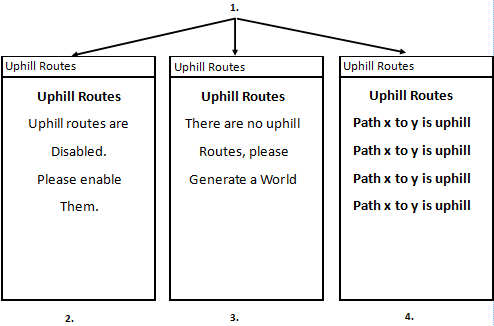
\includegraphics[scale=0.7]{Images/chapter4/uphilviews}
\caption[UphillViewer Design]{Proposal for the UphillViewer interface representing the different states possible at runtime.}
\label{fig:uphillViewImp}
\end{figure}

\textbf{1.} in figure \ref{fig:uphillViewImp} is used to demonstrate each possible state for the UphillViewer contained in the same high level container. \textbf{2.} is used to show the default state and content for the UphillViewer interface. This state is shown to the user if uphill route generation is currently disabled, and prompts the user to enable them. \textbf{3.} is shown to the user if uphill routes generation is enabled, but the current world is yet to be generated. \textbf{4.} is shown to the user when both uphill route generation is enabled and such routes have been generated. The $x$ and $y$ values in this figure will be replaced with indexes of valid cities to enable to the user to understand which routes are deemed uphill.

%4943 WORDS AS OF THIS POINT
\subsection{CityDetail View}
\label{deetzlview}

The CityDetailView is used to summarize how many agents are currently at each City. This view was not initially designed however, the author felt that this was a necessary addition and therefore designed a rough outline of such interface.

\begin{figure}[H]
\centering
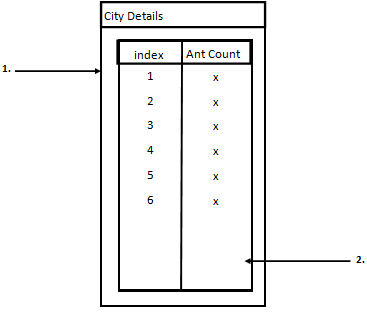
\includegraphics[scale=0.7]{Images/chapter4/citydetails}
\caption[CityDetailViewer Design]{Proposal for the CityDetailViewer interface.}
\label{fig:deetzViewImp}
\end{figure}

\textbf{1.} in figure \ref{fig:deetzViewImp} represents how this view is contained in a separate container to the main display. This enables the user to move this view around as desired in order to customise the current view to their liking. \textbf{2.} demonstrates how the contents of the CityDetailView will be displayed (see section \ref{view:clss}). The number of rows will directly relate to the number of City objects in the current collection. The $x$ values will be substituted for the correct number of ants at the corresponding city index.

\subsection{EquationFrame}
\label{eqnlview}

The Equation Viewer is used to explain the functions that the underlying algorithm uses. This view was not initially designed however, the author felt that this was a necessary addition and therefore designed a rough outline of such interface.

\begin{figure}[H]
\centering
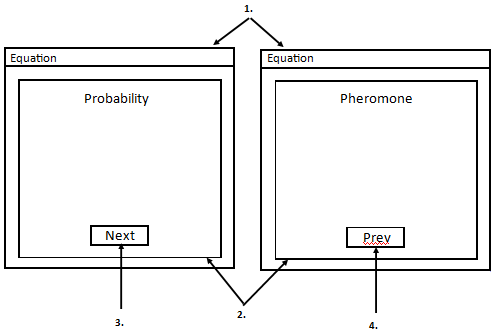
\includegraphics[scale=0.7]{Images/chapter4/pheroprobpanels}
\caption[EquationFrame Design]{Proposal for the EquationFrame interface.}
\label{fig:eqnViewImp}
\end{figure}

\textbf{1.} in figure \ref{fig:eqnViewImp} represents how this view is contained in a separate container to the main display. This enables the user to move this view around as desired in order to customise the current view to their tastes. \textbf{2.} demonstrates how there will one shared panel which will be used to display the content related to both the pheromone and probability equations. The content of the container signified by \textbf{2.} will be substituted for the correct content when the user interacts with either one of the buttons signified by \textbf{3.} and \textbf{4.}. If the user interacts with the button \textbf{3.} then the content of the container will switch and will now represent details about the pheromone equation. When button \textbf{4.} is pressed by the user, the content of the container will now reflect the information stored about the probability equation. The author has designed this such that any additional equations can be implemented in the same way using simple button navigation without the need of significant extensions to the existing framework.

\subsection{Error Feedback}
The interfaces responsible for error feedback have been carefully designed so that the author can effectively inform the user of the error, the cause of the error, and solution of such error. These interfaces are designed to be abstract in such a manner so the same interface can be used to represent several different related error responses.

\subsubsection{Parameter Errors}
\label{paramerror}
These errors are produced when a user has defined a value for an algorithm parameter which is deemed to be illegal. This illegal value could mean that the value the user has entered is outside of the scope of accepted value or the user has specified an illegal type for this parameter. An illegal type a situation such as entering a double value where an integer is required.

The design for these error messages remains as shown in section \ref{error:proposal}, appendix B. This design is simple and effective and provides the user with everything they need to know about the errors source and solution. This interface can be re used for any parameter related error as the only modification would be the change of the interfaces content, there would be no need to implement or design a new interface.

\subsubsection{File IO Errors}

The ability for a user to load or save a problem configuration to a selected file is a new addition to the system. The design of these error interfaces is based off of the design for the parameter error interfaces described in section \ref{paramerror}. 

\begin{figure}[H]
\centering
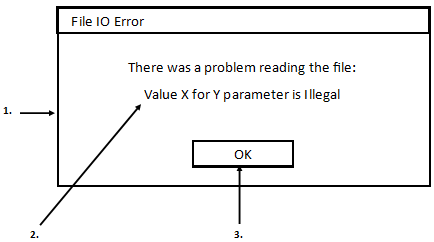
\includegraphics[scale=0.7]{Images/chapter4/IOError}
\caption[File IO Error Feedback Design]{Design of the File IO error feedback interface.}
\label{fig:ioErrors}
\end{figure}

Similar to the parameter error interface, this interface as described in figure \ref{fig:ioErrors} will provide the user with concise feedback as to how and why the file IO process did not complete as expected. From the error message displayed the user should be able to deduce their own solution to the problem. As there are numerous problems which could arise with file IO, the author decided to omit providing a solution to the user. Instead the erroneous data is flagged to the user enabling them to locate the problem and resolve it. The $x$ value in figure \ref{fig:ioErrors} will be replaced with the problematic value whereas the $y$ value will refer to the problematic parameter.

\section{Algorithms}

This section covers the abstract implementation of the key algorithms used for both modelling the algorithms execution and the visualisation of such process.

\subsection{General Overview}

The general algorithm remains largely unchanged from the initially proposed algorithm in section \ref{algym8}, appendix B. The author has amended this design slightly to factor in the change of problem representation. As the TSP is the default problem representation the initial ideas behind ants collecting food and returning to the nest have been replaced by conditionals reflecting if an agent has visited every City or not.

\begin{algorithm}[H]
\caption[Ant System Pseudo-code]{Pseudo-code for Ant System implementation}
\label{aco:pseudo2}
\begin{algorithmic}[1]
\State Initialise AntColonyOptimisation with defined parameters
\If{$!parameters\ are\ legal$}
\State Display error message to user
\State $return$
\EndIf 
\State \textbf{end if}
\State Initialise World with algorithm parameters
\State Initialise $Nodes$ and graph
\State Initialise \textit{pheromone} values
\State Initialise $Agents$
\While {$!all\ agents\ finished$} 
\ForAll{Agents}
\While{!visited\ all\ $City$\ locations}
\State Calculate next move using probabilistic function 
\State Add location to Agent's memory
\State update pheromone
\State Update the View
\EndWhile 
\State \textbf{end while}
\EndFor 
\State \textbf{end for}
\EndWhile
\If{$\textit{local best solution} < \textit{global best solution}$}
\State $global best = local\ best\ solution$
\EndIf
\State \textbf{end if}
\State \textbf{end while}
\State output \textbf{global best} solution
\end{algorithmic}
\end{algorithm}
%5854 words up to this point

This pseudo code remains largely unchanged from the initial design represented by algorithm \ref{aco:pseudo}, appendix B. There has been the modification of the conditional statement represented by line 12 in algorithm \ref{aco:pseudo2}. This change reflects the updated problem representation so that agents now visit all City locations rather than focussing on a nest and food situation.

\begin{sidewaysfigure}
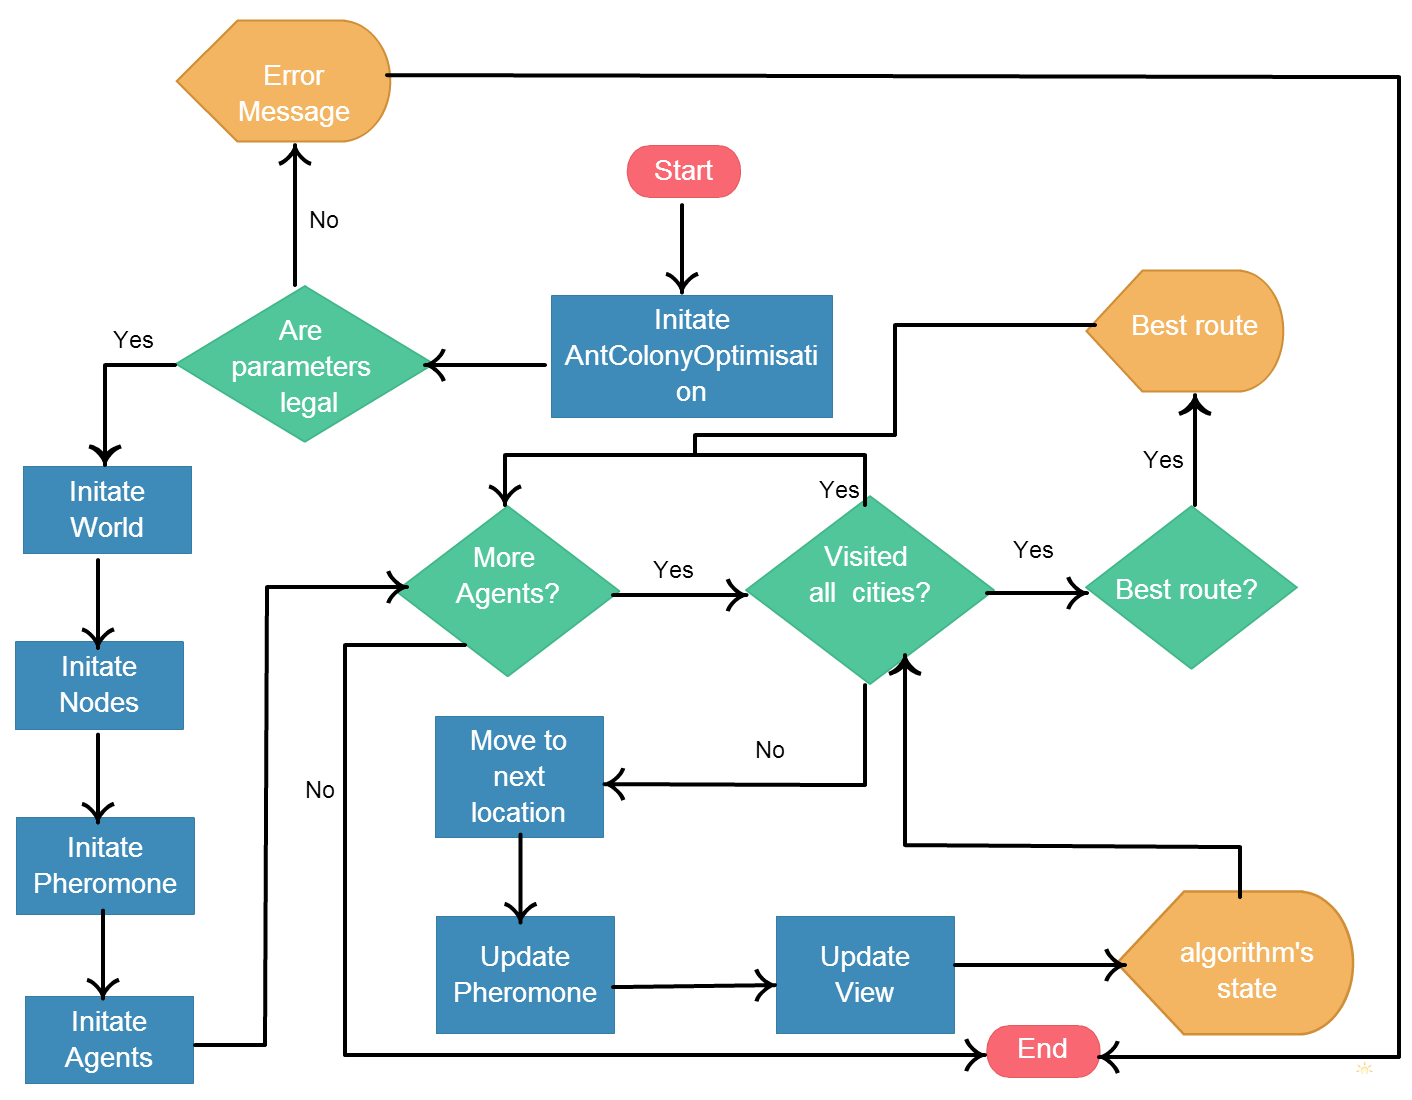
\includegraphics[scale=0.45]{Images/chapter4/overallflow}
\caption[Basic Ant System Flow Diagram]{Flow diagram representing the algorithm described in algorithm \ref{aco:pseudo2}}
\label{fig:overallFlow}
\end{sidewaysfigure}

\begin{figure}[H]
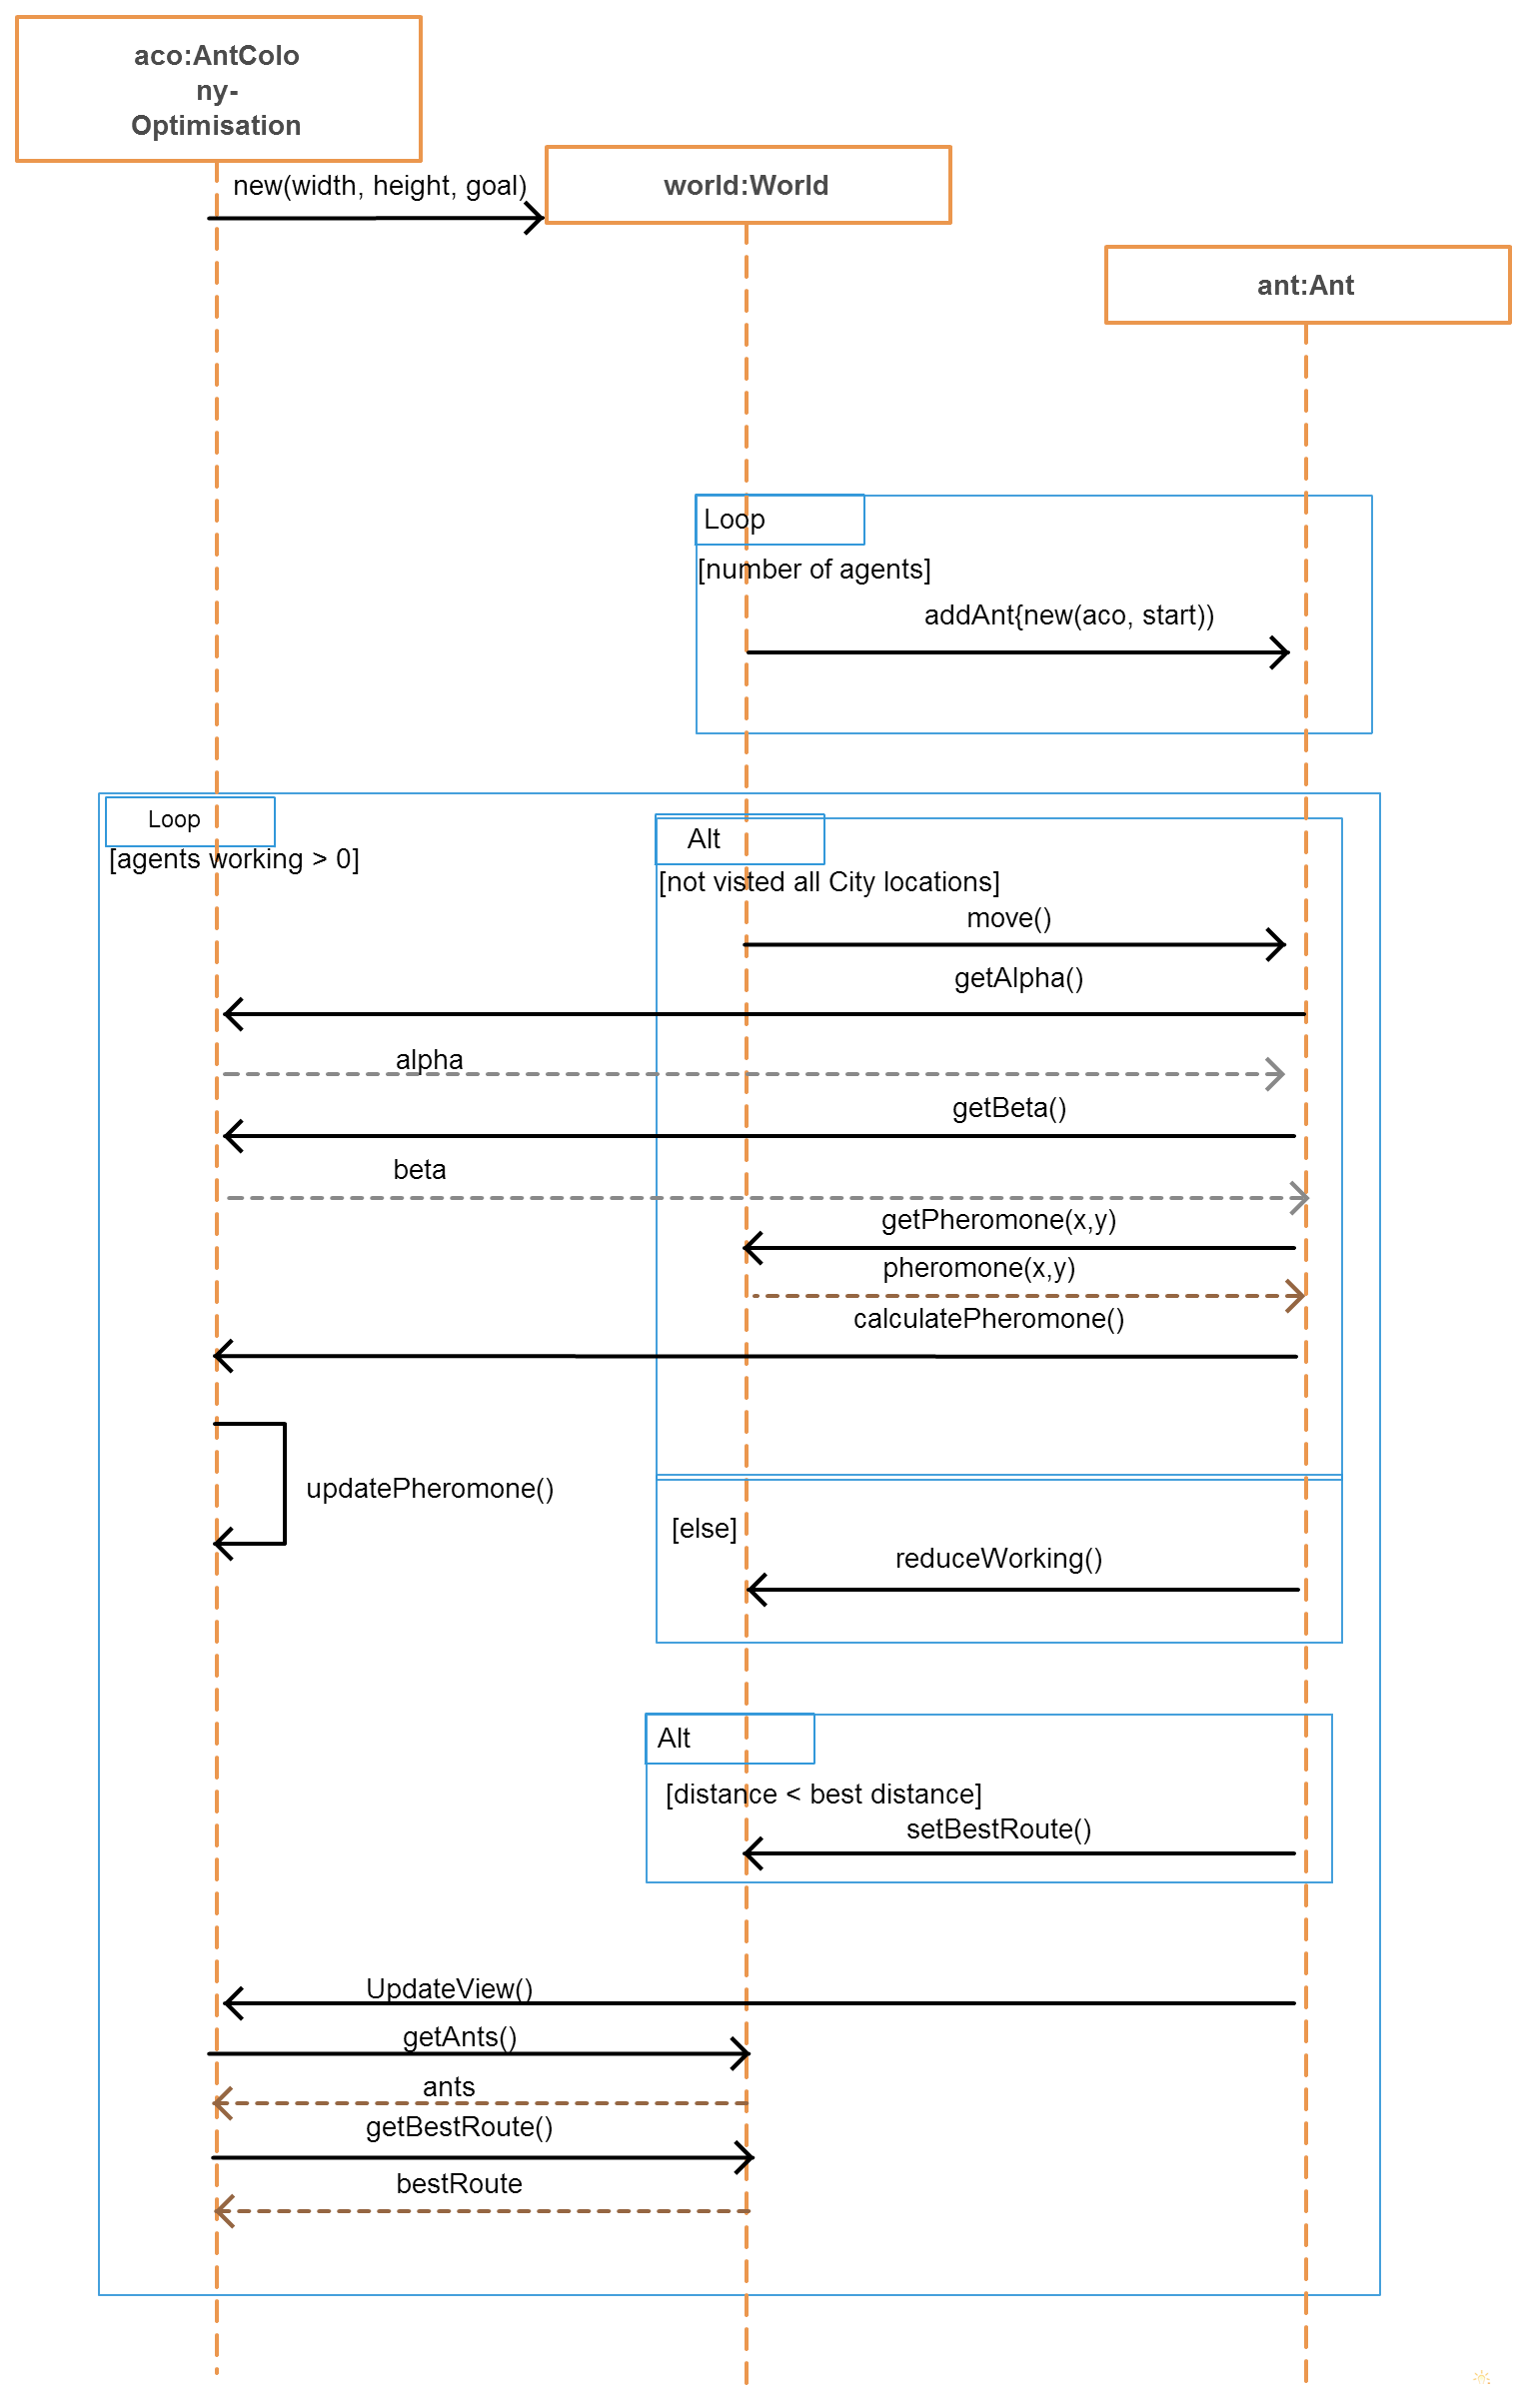
\includegraphics[scale=0.27]{Images/chapter4/sequence}
\caption[Overall Sequence Diagram]{Overview of system interactions based on Algorithm \ref{aco:pseudo2}}
\label{fig:overSeq}
\end{figure}

The sequence diagram described in figure \ref{fig:overSeq} demonstrates at a high level how the algorithm executes. This differs slightly from the initial design (figure \ref{fig:seq}) in order to correctly model the change of problem representation.

\subsection{Formulae}

\subsubsection{Probability}

The probability function is defined in section \ref{sssec:probfuncsssec} appendix B. The design for this algorithm remains unchanged form the pseudo code represented in algorithm \ref{aco:pseudo:probfunc}. The result of this algorithm is in fact, the probability associated with the agent moving to a specific location.

\subsubsection{Pheromone}

The probability function is defined in section \ref{sssec:pherodepo} appendix B. The design for the probability algorithm remains unchanged form the pseudo code represented in algorithm \ref{aco:pseudo:pherofunc}. This is the function that models the pheromone deposit and decay operations.

\subsection{Elitist Ants}

The Elitist Ant algorithm was not initially planned as a feature provided by this application. The author decided that sufficient time was available to produce a brief design for the Elitist ant algorithm extension to allow for a smooth implementation of such design.

\subsubsection{Overview}

The general premise for this Elitist Ant algorithm is defined in section \ref{eliteymcneaty}. The probability function will remain the same as defined in algorithm \ref{aco:pseudo2} whereas the general behaviour of the system and the pheromone deposit function will differ slightly to that of the Basic Ant algorithm. The general system interactions will be the same as shown in figure \ref{fig:overSeq}.


\begin{algorithm}[H]
\caption[Eltist Ant System Pseudo-code]{Pseudo-code for Elitist Ant System implementation}
\label{aco:pseudoEAS}
\begin{algorithmic}[1]
\State Initialise AntColonyOptimisation with defined parameters
\If{$!parameters\ are\ legal$}
\State Dispaly error message to user
\State $return$
\EndIf
\State Initialise World with algorithm parameters
\State Initialise $Nodes$ and graph
\State Initialise \textit{pheromone} values
\State Initialise $Agents$
\While {$!all\ agents\ finished$} 
\ForAll{Agents}
\While{!visited\ all\ $City$\ locations}
\State Calculate next move using probabilistic function 
\State Add location to Agent's memory
\State Update pheromone
\State Update the View
\EndWhile 
\If{total\ stored $Elite Ants\ <$ total\ defined $Elite Ants$}
\State add this ant to elite ants
\Else 
\ForAll{$Elite Ants$}
\State find\ the\ $Elite Ant$ with\ the\ worst\ route
\If{worst\ $Elite Ant$ route is worse than this $Ant$ route}
\State replace\ worst\ $Elite Ant$\ with\ this\ $ant$ 
\EndIf
\State \textbf{end if} 
\EndFor 
\State \textbf{end for}
\EndIf 
\State \textbf{end if}
\State \textbf{end while}
\EndFor 
\State \textbf{end for}
\EndWhile 
\State \textbf{end while}

\If{$\textit{local best solution} < \textit{global best solution}$}
\State $global best = local\ best\ solution$
\EndIf
\State \textbf{end if}
\State \textbf{end while}
\State output \textbf{global best} solution
\end{algorithmic}
\end{algorithm}
%6306 to this point
The difference between aglorithms \ref{aco:pseudoEAS} and \ref{aco:pseudo2} is the manipulation of EliteAnts which is defined in lines 16 to 25. These lines enable the algorithm to constantly ensure that only the best (Elite) $x$ number of ants are stored across iterations to ensure than these pheromone is deposited on the best paths. In order to do this, every time an ant has completed certain checks are made to see if this ant is eligible to become one of the $x$ elite ants. An ant is deemed eligible if the current elite ant collection is not fully populated or if this ant has a better route than the worst performing elite ant. If the later of these two conditions is met then the worst performing elite ant is then swapped with the current ant. This difference can also be observed in figure \ref{fig:overallFlowEAS} which gives an even more abstract overview of the Elitist Ant System.

\clearpage
\begin{sidewaysfigure}
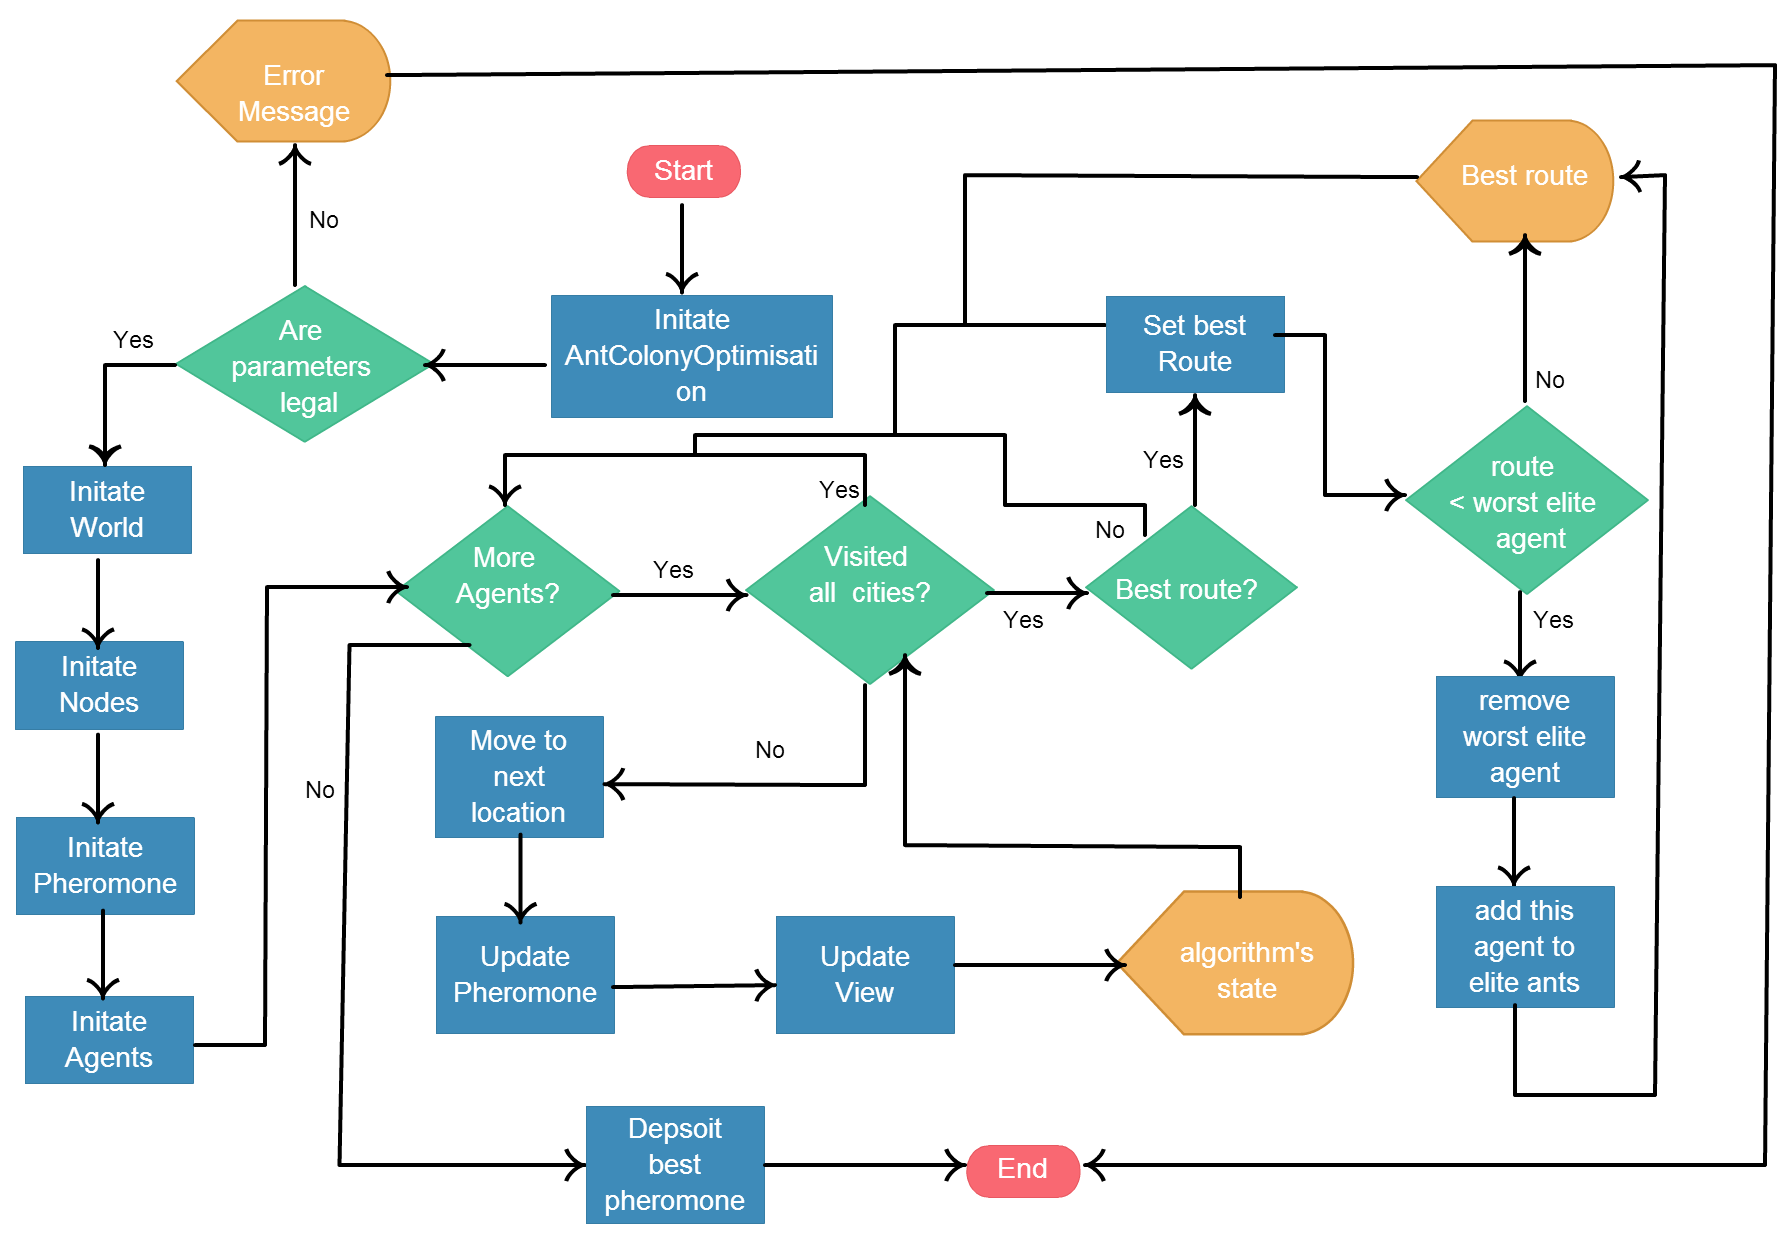
\includegraphics[scale=0.38]{Images/chapter4/eliteAntFlow}
\caption[Elitist Ant System Flow Diagram]{Flow diagram representing algorithm \ref{aco:pseudoEAS}}
\label{fig:overallFlowEAS}
\end{sidewaysfigure}
\clearpage

\subsubsection{Depositing Best Pheromone}

As described in section \ref{eliteymcneaty}, the Elitist Ant System has a slightly different pheromone function to that of the one described in section \ref{sssec:pherodepo} for the Basic Ant system. This modified pheromone function is mostly the same as in the Basic Ant System however, the elite routes must be factored in.

\begin{algorithm}[H]
\caption[Elite Ant System Pseudo-code Pheromone Function]{Elitist Ant System pheromone function pseudo-code}
\label{aco:pseudoEASphero}
\begin{algorithmic}[1]

\State define the $e$ value $=$ $e \times $ \#\ of\ $cities$
\ForAll {stored\ $EliteAnts$}
\State initialise index $i = 0$
\State $currentBest = EliteAnt\ path$ 
\ForAll {$Cities$ along $currentBest$}
\State get the $City\ index$ at $currentBest[i]$
\If{$i + 1 < currentBest\ size$}
\State get the $City index$ at $currentBest[i + 1]$
\State add $e$ amount\ of $new\ pheromone$\ to\ $pheromoneEdge[i][i + 1]$
\EndIf 
\State \textbf{end if}

\State $i++$
\EndFor 
\State \textbf{end for}
\EndFor
\State \textbf{end for}

\end{algorithmic}
\end{algorithm}

Algorithm \ref{aco:pseudoEASphero} demonstrates how the current elite ants are factored into the pheromone function. In general, this will enable the population of agents to converge towards a solution at a faster rate than the Basic Ant System as the increased amount of pheromone on edges used in the current best paths will be greater thus, ants will have a greater probability of traversing such edges.

\subsection{Algorithm Rendering}

Design and development of the algorithm responsible for visualising the Ant Colony algorithm's current state  is one of the more important algorithms in the application as the visualisation process is key to the projects success.

\begin{algorithm}[H]
\caption[Algorithm Visualisation Pseudo-code]{Pseudo-code for rendering of the algorithms execution}
\label{aco:renderPesudo}
\begin{algorithmic}[1]

\State retrieve latest version of the model
\If{model $!null$}
\ForAll{$Cities$ in $model.getWorld().getCities()$}
\State $drawOval(City.X, City.Y, width, height)$

\If{algorithm $!finished$}
\For{$City$}
\ForAll{$Cities$}
\State set opacity based on pheromone value at $edge[city.index][cities.index]$
\State draw a line from $City_{xy}$ to every element in $Cities_{xy}$
\EndFor 
\State \textbf{end for}
\EndFor 
\State \textbf{end for}
\EndIf
\State \textbf{end if}
\EndFor
\State \textbf{end for}
\ForAll{$agents$}
\ForAll{$cities$}
\If{$agent\ location == City.index$}
\State draw agent at $City.x, City.Y$
\State $break$
\EndIf
\State \textbf{end if}
\EndFor
\State \textbf{end for}
\EndFor
\State \textbf{end for}
\If{$best distance > 0$}
\State $best\ route = model.getBestRoute()$
\For{$i = 0$ untill $i <$ $best\ route.size()$}
\If{$i + 1 < \ best\ route.size()$}
\State set colour as red
\State $drawLine(Cities[i].x, cities[i].y, cities[i + 1].x, cities[i + 1].y)$
\EndIf
\State \textbf{end if}
\EndFor
\State \textbf{end for}
\EndIf
\State \textbf{end if}
\EndIf
\State \textbf{end if}

\end{algorithmic}
\end{algorithm}
%6834 untill here

The pseudo code represented in algorithm \ref{acorenderPesudo} defines the design of the general concept used to visualise the underlying algorithm. The author acknowledges that this is not the most efficient or elegant design and this is used an implementation starting point and is by no means a concrete design. Lines 3 to 13 are used to represent the graph visualisation. Drawing a line from every City to every other City will simulate a fully connected graph of cities to the user. The opacity of these lines will be be directly related to the pheromone concentration for the corresponding edge. Lines 22 to 30 show way in which the current best path will be rendered to the user. The author has designed this so that multiple pairs of lines are drawn which will ultimately form one continuous line representing the best path. Each line will have a start and end location, the end location of each line will become the starting location of the next line. This is done by iterating through the pairs of the cities in the best route until there is no longer a valid pair of locations to draw a line between. Once this point is reached the line is complete.
\chapter{Implementation PUT IN OWN FILE}

\section{User interface}
\label{mainimp}
The main display represents the general interface is displayed to the user. This is where the algorithms visual representation will be presented, as well as providing the location of the user interaction elements enabling modification of the algorithms parameters. This interface is a result of the contents of the DisplayFrame Class and its contents. The design for this view is almost as described in section \ref{ssec:mainUI}, appendix B, however, there has been a slight modification to this proposed design.

\begin{figure}[H]
\centering
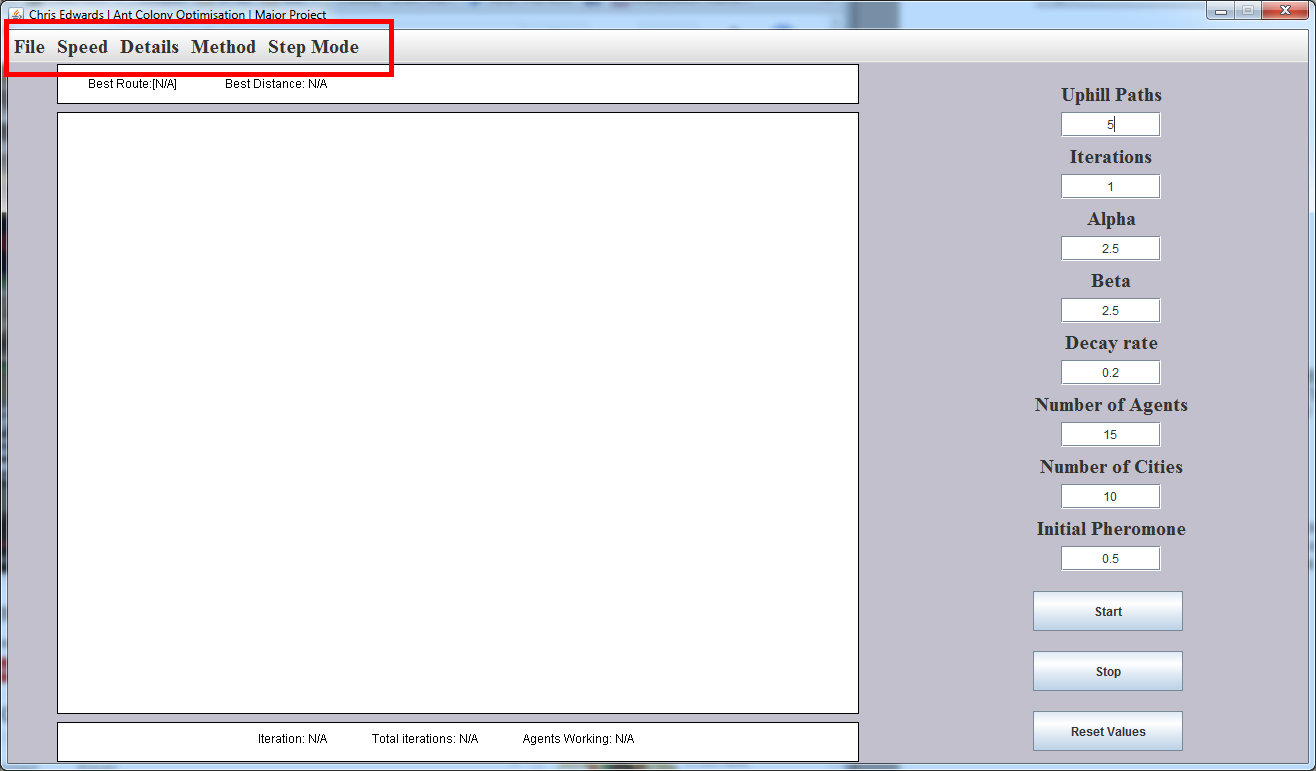
\includegraphics[scale=0.35]{Images/chapter4/displayFrame}
\caption{Implementation of the proposed user interface. The contents of the red polygon highlights the additional features not present in the initial design.}
\label{fig:displayFrameImp}
\end{figure}

The additional features highlighted by the red polygon in figure \ref{fig:displayFrameImp} represent the features which were not initially designed. These features are represented in a separate location to the control panel (right hand side of figure \ref{fig:displayFrameImp}) as there is no logical connection between the menu bar features, and the modification of the algorithm parameters. The author opted to use a menu bar to control the access to these features as the vast majority of users will recognise what a menu bar is, and understand how to interact with such elements. 

The different elements contained in this menu bar relate to general system interactions. The File option enables the user to either load, or save a configuration to a specified file. The Speed option enables the user to change the Thread speed, which will directly change the algorithms rate of execution. The Details menu is used to control access to any additional views. The views which can be access here are; the Uphill Viewer (section \ref{uphillview}), The City Detail View (section \ref{deetzlview}) and the Equation Viewer (section \ref{eqnlview}). In addition to the access of these extra views, the Detail menu also enables the user to disable and enable uphill routes \Large REFERENCE UPHILL ROUTES GENERATION ALGORITHM PSEUDO CODE \normalsize to be generated for current problem. The Method option enables the user to select the current algorithm type from a list of implement algorithm types. Currently the author has implemented a Basic Ant System and an Elitist Ant system so the user can switch between these algorithm types. The Step Mode menu enables the user to enable or disable the step mode functionality. When enabled, step mode will allow the user to step through the algorithms execution at their own pace without the application automatically solving the problem.

\section{Data Structures}

\subsection{Pheromone and Distance Matracies}

\subsubsection{Pheromone}
\label{phero:struct}
A Pheromone Object is used to represent the pheromone concentration for a given edge in the current problem graph, however there is no data stored inside the Pheromone Object which relates this Object to a specific edge. To enable logical indexing of these Objects such that the author could continually the pheromone data for a specific edge is a fairly trivial task however, the method of doing so has changed since the initial proposed design as seen in section \ref{pheroRepsec}, appendix B.

The concept of a using two-dimensional array to store the pheromone data is still present however, the dimensions of such structure are now directly representational of the number of cities present in the current problem. Assume there are $x$ number of cities in the current problem then the length of each array would also become $x$. Therefore the instantiation of the pheromone data structure is of the format $Pheromone[][] pheromone = new Pheromone[x][x]$. Assuming these $x$ cities have the $index$ values $0, 1, ..., x-1, x$ then indexing any edge would be done using the format $pheromone[x][y]$. Given this format, $x$ and $y$ are any valid $City indexes$. For example, to access the pheromone concentration for the edge corresponding to the path from $City\ 0$ to $City\ 5$ would be accessed using $pheromone[0][5]$. As accessing an element in in an array is a $O(1)$ operation this method of access is extremely efficient and supports a problem of almost any size as the data structure resizes with the problem. Figure \ref{initPheroCode}, appendix C represents how the pheromone matrix is initialised using the initial pheromone value for all edges.

\subsubsection{Distance Matrices}

Initially there was no proposed design for the inclusion of data structures representing the distances between each node in the graph as the initial design for the problem representation made it simple to calculate the distance between the current node and the destination node extremely trivial. The author decided that as the problem representation has changed to the TSP there needs to be a better method of accessing the distances between two nodes (Cities).

The design for the distance matrices are based on the implementation provided by Thomas Jungblut \cite{tjung:aco:blog}. The implementation of these data structures is identical to that discussed in section \ref{phero:struct} however, the data stored in each array element represents the $euclideanDistance$ between two $cities$ rather than the pheromone concentration. As defined in section \ref{phero:struct} the size of distance matrices will represent the number of cities. If there are $x$ cities in the current problem then the format for instantiation will be $double[][] distanceMatrix = new double[x][x]$. The way in which elements are accessed also remains the same as above, however once instantiated these values will remain constant as a $City$ cannot move location. These matrices are easily populated after the cities have been instantiated. The code in appendix C figure \ref{initDistanceCode} represents how this has been implemented. A correct implementation would return a distance of $0.0$ if $index[x][x]$ were to be accessed where $x$ is the same value. This is because the distance from any $City$ to itself is 0.
As the probability is represented as $p_{xy}^{k} = \frac{(\tau_{xy}^{\alpha })(\eta _{xy}^{\beta })}{\sum (\tau_{xy}^{\alpha })(\eta _{xy}^{\beta })}$ where $\eta _{xy}$ represents $\frac{1}{distanceMatrix[x][y]}$ (inverted distance). As this function is used extremely often during the algorithms execution rather than converting the value of $distanceMatrix[x][y]$ every time an inverted version is needed it is far more efficient to store an inverted version of the $distanceMatrix$. The code snippet in appendix C, figure \ref{initInverteddistanceCode} demonstrates how this can be implemented. The $invertDouble(distanceMatrix[i][j])$ in said figure simply returns the value of $\frac{1}{distanceMatrix[x][y]}$ however if $distanceMatrix[i][j]\ ==\ 0.0$ then $0.0$ is returned as $\frac{0}{distanceMatrix[x][y]}$ is illegal.
  
\subsection{Agent and City Collections}

Both Agent and City Objects are designed to be stored using data structures which implement the List$<$type$>$ Java interface. As the number of Cities and Agents present in the current problem is dynamic and user defined the size of the data structure must be established at runtime and therefore the data structure chosen must scale well and maintain performance regardless of its size. In addition to this, a user is able to modify the amount of Agents and Cties once created, therefore the data structure must be able to be effectively resized dynamically without complication. The ArrayList data structure has been chose to store the Agents and Cities as it is scalable and can be dynamically resized. An Array implementation could be used here however, if the Array reached capacity then there would need to be conditionals put in place by the author to copy the contents of the full Array into a new, larger Array instance. The use of ArrayList means that the author does not have to worry about these conditionals are they are handled for the author by the ArrayList implementation. In addition to this, the order the elements in generally unimportant, accessing a random index however is. Using an ArrayList provides $O(1)$ random element access using the provided $get(index)$ method. Also inserting into an ArrayList is $O(1)$ where as an Array implementation would provide $O(n)$ insertion as the next free index would have to be located. As the ordering in unimportant there is no reason to use a LinkedList data structure and the improved performance of the ArrayList versus an Array has enabled the author to confidently select an ArrayList implementation as the best suited data structure. 

Unless explicitly stated by loading a configuration from a file, the locations of the $City$ elements in collection of cities are randomised. There are conditionals in place to ensure that two cities cannot be placed in the same location as this is a possibility if the locations of such cities is random. The implementation of the $City$ instantiation can be found in appendix C, figure \ref{initCity}.

The starting location of the Ant Objects represented as elements in the collection of agents is also randomised. This random value is however limited to a range of integers with a maximum possible value equal to $cities.size() - 1$. As indexes start at 0, this enables the random function to return any $City$ index such that it is possible for an agent to start at any $City$ location. The implementation of this agent instantiation is defined in appendix C, figure \ref{initAnt}.

\subsection{Best Route representation}

Storing the current best route is slightly more complicated than storing the collection of Agents or Cities as the ordering is important. As the ordering is important the accessing of random indexes is irrelevant as the elements stored in this data structure when parsed in order represent the order to cities which the agent visited in order to produce this best route. The indexing of random elements would enable the elements to be parsed in an incorrect order, thus this functionality will not be used by the author and therefore the data structures performance in executing such task is completely nullified. The data structure used for this representation does not need to have dynamic resizing capabilities as the length of any best route will represent the number of cities in the problem as an agent must visit every City once and only once. The author reduced his choice to using an ArrayList or a LinkedList implementation. A LinkedList implementation has massive performance enhancements when compated to an ArrayList as a LinkedList can provide constant time ($O(1)$) insertion and deletion operations using iterators which can be relied upon regardless of the magnitude of such data structure in combination with the lack of regard to element ordering. An ArrayList cannot reliably provide such performance. This in addition to the fact that the ordering of elements is important, has lead the author to decide on using a LinkedList data structure for the representation of the best routes.

\section{Pheromone Operations}

The translation of the pseudo-code described in algorithm \ref{aco:pseudo:pherofunc} was a fairly simple process as the pheromone algorithm is itself relatively simple. Once implemented the author quickly realised that the pheromone operations (deposit and decay) were not behaving correctly. During the course of agents $move()$ method every time the agent moves from its current location to its next location pheromone proportional the distance travelled would be deposited on the corresponding edge. The problem was that every time this pheromone was deposited the global pheromone was in fact being decayed so the global pheromone was being decayed every time the agent moved. In order to prevent this problem from arising rather than directly updating the pheromone on the edge when the ant moves the agents pheromone deposit on this edge is instead added to a secondary $newPhero$ variable in the Pheromone Object for this corresponding edge. This variable is used to collate the total amount of new pheromone to be deposited for any edge. When it is time to update the edge pheromone, every Pheromone Object is iterated through and value present in this $newPhero$ variable is used in the pheromone calculation allowing for correct behaviours to be represented. This is slightly more complicated than the author envisioned however, the additional complexity is essential to ensure correct behaviour. The implementation of this method is shown in appendix C, figure \ref{codephero}.

\section{Solving the Problem}

The author encountered unforseen complications when implementing the pseudo-code represented in aglorthm \ref{aco:pseudo2}. The subsections below described the problems with the implementation process and their associated solutions.

\subsection{Agent Movement}
\label{antyMove}
The author has problems initially with his implementation of the probability based movement of the agents. The implementation of the Ant's $move()$ function worked as expected there were no complications assoicated with that however, the complication that the author encounted involved the probabilistic selection of the Ant's next location. The problem caused every Ant that started at the same City index to take exactly the same route. Upon debugging the Ants $getNextProbableNode(int y)$ function the author realised that there was in fact no random element assoicate with this method and the City with the highest probability was constantly selected thus, the Ants never had the ability to divert away from the best looking route causing local solutions to be present. The author attempted to implement this random element into his method however the aglorithm did not perform as effeciently as expected. Thomas Jungblut had provided an open source implementation of a basic Ant Colony Optimisation algorithm \cite{tjung:aco:blog}. This implementation was provided free of charge and allowed modification which enabled the author to replace his lackluster node selection function with a the one provided in this working implemention. This node selection function did however require modfication by the author to ensure correct operation with his architecture. Once this method had been modified and implemented the node selection process for the Ant's next location worked as initially intended. The author realised that his implemention took completely the wrong approach which involved sorted the candidates locations based on thier assoicated probability. Had the author not accepted that the re-use of a working implemention is the best way to progress the application then a reduce in project quality would have been a possibility.  The implementation of this node selection method can be seen in appendix C, figure \ref{nextNodeCode}. If this method returns $-1$ then the Ant is deemed to have completed its walk.

\subsection{Automated Solving}
\label{autoSolve}
Implementing an algorithm which once started, executes untill completion was in fact fairly simple to do initally. This simplistic implementation stemmed from the fact that initially the aglorithm only considered the fact there was one iteration. As there was one interation it was simple to define a stop condition which was in fact when every agent had completed its walk which meant the aglorithm stoped when $Ant.getFinished()\ returned\ true$ for every Ant. Once the author had impleted automatic execution for one interation, the ability for a user defined number of interations was implemented. The addition of the to support $x$ number of iterations where$x\ >\ 1$ introduced several new complications. Each new iteration meant that the Ants need to be reset so that they forget everything from the previous iteration(s) but the pheromone levels, Cities and current best route must all be persevered accross iterations. In order for this to be possible, the author adpated to algorithms stop condition to now be relative to the number of iterations or in other words stop when $currentIteration\ ==\ totalIterations$. A new iteration is started when all Ant's have finished thier walk, instead of checking every Ant for the condition $Ant.getFinished()\ ==\ true$ once an ant had finished a variable representing the total number of Ants current working (unfinished) was reduced by 1. When this value reaches 0, there are no Ants currently working thus the iteration has completed. Once an iteration has completed the Ants must be reset so the next iteration can start, this is done by calling the $initAnts()$ method again on the current $World$ enabling the old Ants to effectively be reset. The variable representing the number of Ants working is also reset so that $antsWorking\ ==\ totalAnts$ and the process starts again. During this reset operation the pheromone levels, cities and best route remained unchanged to ensure previous iteration results remian. The implementation for this algorithm can found in appendix C, figure \ref{iterationThing}.

\subsection{Step Based Iteration}

In order to implement an algorithm which executes one step and a time and requires contant user interaction in order to execute to completion several modifications have to be made to the algorithms used in the proceess of automated solving. The first problem associated with step based iteration is the fact that an Ant must be stopped moving after it has moved to its next location, in comparison the fully automated approach uses an algorithm which ensures an Ant continues moving untill it is finished or move while the aglorithm in figure \ref{nextNodeCode} does not return $-1$ . In order to stop the Ant after one movement the algorithm in section \ref{antMove} can remain largely the same, however this while loops must be removed so that the movement function executes once and only once per step. This change alone however is not enough to stop the aglorithm from executing untill completion. Rather than using a $for\ each$ loop to iterate through every Ant and instructing it to move as decribed in figure \ref{iterationThing} there must now be a way to track the current Ant which is moving and updated this tracker once said Ant is finished. In order to do this an index representing the location of current working Ant is stored so that when the aglorithm is stepped through only the Ant and that index is signaled to move 1 step. Once this Ant has finished, then this index is incremeneted untill $index\ >=\ agentsCollection.size()$. Similar to the aglorithm descirbed in section \ref{autoSolve} once every Ant has finished walking, the iteration is complete and if there are more iterations to execute then the Ants and index are reset. The implementation of this step based iteration can be seen in figure \ref{stepM8}.

\section{Rendering the Algorithm}

The implementation of the pseudo-code represented in algorithm \ref{aco:renderPesudo} turned out to be far more complicated than the author actually planned. The subsections below segment the complications that arose and the steps the author took in order to ensure a proper visualisation process.

\subsection{Swing Worker}

\subsection{Visualising Agent Movement}

\subsection{Scaling}

\subsection{Painting the Canvas}

\section{Elitist Ants}

\section{Uphill Routes}

\section{File IO}

\section{Requirement Evaluation}

The implementation should look at any issues you encountered as you tried to implement your design. During the work, you might have found that elements of your design were unnecessary or overly complex; perhaps third party libraries were available that simplified some of the functions that you intended to implement. If things were easier in some areas, then how did you adapt your project to take account of your findings?

It is more likely that things were more complex than you first thought. In particular, were there any problems or difficulties that you found during implementation that you had to address? Did such problems simply delay you or were they more significant? 

You can conclude this section by reviewing the end of the implementation stage against the planned requirements. 



\chapter{Testing}

\section{Overall Approach to Testing}

This chapter presents a multitude of different testing types. There are automated unit tests to ensure the internal code logic behaves as expected. The User Interface tests are tests which are difficult to automate but are used to ensure that the user interface models the correct state of execution. Acceptance testing is used to assess how well the applications meets the specified requirements in section \ref{funcymcdunky}. Stress testing has been considered by the author but ultimately has been omitted. The author feels that the application is never subject to heavy loads, nor can the user exceed the normal operational load for the application. Overall the testing process is not as thorough as the author desires, given the short time frame for the projects development the author feels that the testing suffices in ensuring correct functionality.

\section{White-box Testing}
\subsection{Unit Tests}

There are features present in the application code which the author has excluded from the unit testing process. Any feature which relies on random numbers to perform its task has not been unit tested. The author feels that any methods which uses a random number can’t reliably be tested therefore, it doesn’t makes sense to attempt to. Instead the author has extracted the code which relies on such random numbers and tested the behaviour of such code using specifically defined values, this enables the author to accurately test for expected behaviours. In addition to this getter and setter methods or simple assignment operations have not been tested. The reason for excluded these methods from unit tests is because the code responsible is so simple it can’t fail so there is no real purpose in producing such tests.

The unit tests that the author has produced revolve around ensuring that only legal algorithm parameters are accepted and that the movement, probability and pheromone functions are behaving as expected and return legal values. These tests contain validation checks against a range of values for each parameter including boundary conditions to ensure that they are correctly dealt with, examples of such testing can be seen in figures \ref{testAlpha} to \ref{testAgent}. An example of such testing can be seen in figure \ref{testProb} which tests that the calculated probability sums to 1. There are many more tests present in the test package for the application however the author has only briefly outlined a small number of these. Evidence of such testing can be seen below in figure \ref{testSS}.

\begin{figure}[H]
\centering
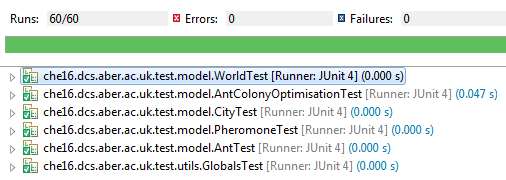
\includegraphics[scale=0.8]{Images/chapter6/testSS}
\caption[Unit Testing Summary]{Evidence of the completed execution of the applications unit tests. The view present is the built in Eclipse JUnit interface.}
\label{testSS}
\end{figure}

\section{Black-box Testing}
\subsection{User Interface Testing}

It is difficult to reliably test the graphical user interface using a white-boxing testing approach. To overcome this obstacle the author has decided to manually test the user interface using a black-box testing approach to ensure the correct behaviour is exhibited.

During this test process the author did not repeat any test previously executed in the unit testing process. The tests performed manually by the author will be for the purpose of ensuring that the correct error messages are displayed to the user in the correct situation and making sure the algorithm is being correctly rendered.

In addition to testing for errors the file IO process will be tested ensure that configurations can be correctly loaded and saved to a specified file. Several test files will be produced. Each file will be designed to test a variety of possible legal and illegal file contents. Tests will be done to ensure that the application rejects files that contain; missing data, incorrect type for a specified value and City coordinates which exceeds the bounds of the canvas. The saving of a configuration to a file doesn’t not need to be as rigorously tested as the algorithm has to be instantiated with legal values before the writing process can be executed therefore, the values of the written file will be legal and of the correct format. An example of such file contents can be found in appendix D, section \ref{fileIOtest}. The full list of black-box test performed by the author can be seen in section appendix D, section \ref{UITESTSM8}.

\subsection{Acceptance Testing}

Due to the lack of a dedicated client acceptance testing proved difficult for this project. For the purpose of these acceptance tests the author acted as the end user, and used the application in a non-bias manner and adapted the mind-set of a new user. This is far from an ideal way to perform acceptance tests and this process isn’t truly representative of true acceptance testing. The application itself is not a finished deployment ready product. Before this would be the case the author would like to extend current functionality and provide a larger variety of algorithm types and modifiers. If the author had a larger time frame then a distinct customer or user group would be set up to ensure this acceptance testing process is performed to the highest quality. Similar tests have been grouped together, the results of this process can be found in appendix D, \ref{AcceptanceTestz}.
% add any additional chapters here

\setemptyheader
\addcontentsline{toc}{chapter}{Appendices}
\chapter*{Appendices}
\pagebreak

% start the appendix - sets up different numbering
\fancypagestyle{plain}{%
%\fancyhf{} % clear all header and footer fields
\fancyhead[L]{\textsl{Appendix\ \thechapter}}
\fancyhead[R]{\textsl{\leftmark}}}

\appendix
\fancyhead[L]{\textsl{Appendix\ \thechapter}}
\fancyhead[R]{\textsl{\leftmark}}
\fancyhead[C]{}
\fancyfoot[C]{\thepage}
\renewcommand{\headrulewidth}{0.4pt}
\renewcommand{\chaptermark}[1]{\markboth{#1}{}}

\fancyhead[L]{\textsl{Appendix\ \thechapter}}
\fancyhead[R]{\textsl{\leftmark}}
\fancyfoot[C]{{\thepage} of \pageref{LastPage}}

% include any appendices here
\documentclass[10pt,a4paper]{article}
\usepackage[margin=1.2in]{geometry}

\begin{document}
\begin{titlepage}
    \begin{center}
        \vspace{1cm}
        
        \Huge
        \textbf{Visualising Ant Colonoy Optimisation}
        
	 \vspace{0.5cm}
        \Large
	 \textbf{Version:} 1.0 Draft \\
        G400  Computer Science, CS39440
	  

        \vspace{1.0cm}
        
	  \Large
        \textbf{Author:} Christopher Edwards \\
         che16@aber.ac.uk

 	  \vspace{0.8cm}
 	  \textbf{Supervisor:} Dr. Neil MacParthalain \\
         ncm@aber.ac.uk
        
        \vspace{3.0cm}
        
        A requirements  specification for a Computer Science Major Project
                
        \vspace{0.8cm}
                
        \Large
        Department of Computer Science\\
        Aberystwyth University\\
        Wales\\
        
        
	\end{center}
\end{titlepage}


\section{Introduction}

\subsection{Purpose}

The purpose of this document is to give a detailed description for the `Visualising Ant Colony Optimisation' application. This document will cover the interface interactions and methods as well as providing definitions to important terminology. The document is primaraly intended to be used as a reference point for the initial stages of development.

\subsection{Scope}

The `Visualising Ant Colony Optimisation' application is a desktop application which is designed to demonstrate the behaviour of an underlying ACO algorithm given various algorithm parameters. These parameters will be defined by the user and can be modified at their convenience. The algorithms behaviour given these parameters will be visible and the users can make a clear assessment about how each of the parameters impacts the algorithms performance.

During the background research into this subject area there does not seem to be too many applications which offer ACO visualisations and there are even less which provide a `friendly' environment which is simple and intuitive to use regardless of the users background knowledge in regards to the subject area.

The software will be deployed in an educational environment, and aims to provide a means for teaching ACO to students as part of an Artificial Intelligence course or for independent use as a self-learning exercise. As a result the software must cater for the majority of user groups to maximise its effectiveness. This means the software must be accessible on all major platforms and perform equally well on said platforms.

\subsection{Definitions}

\begin{table}[h]
\centering
\begin{tabular}{|l|l|lll}
\textbf{Term} & \textbf{Definition}                                            \\ 
\hline
ACO           & Ant Colony Optimisation                              \\ 
user          & Anybody who is using or wishes to use the software      \\ 
user group    & A collective group of users representing different user needs. \\ 
interface       &A graphical user interface \\
standalone    &Operates independently of other hardware or software\\
agent		&The entities which will be traversing the graph \\
\end{tabular}
\caption{Definitions for the keys terms used throughout this document}
\end{table}

\section{Overview}

This section will give an overview of the proposed application. This section will also expand on the expected user groups and functionality required by said groups. The constraints 

\subsection{Product Descriptive}

The software application will be standalone and does not need to communicate with another system or application, because of this there is no need for any form of network connection to be present in order to use the application to its maximum potential.

The application will communicate with the Operating System on the host machine in order to enable the save and load functionalities through simple file input and output. However the user’s access to the host machines file system will be restricted by the fact that the saving and loading will be restricted to the user’s home directory preventing the overwriting of important documents.

The application itself will not take up too many system resources even if a large problem is being handled. This allows the users on a system or network to run the application without it impacting the performance of other services. Given that the target audience is educational establishments this is especially important as many teaching fellows have multiple applications running during a lesson or lecture and a negative impact on their system could reduce the amount of information taught during said session.

\subsection{Product functionality}

The users will be able to view a world which represents the Agents and the nodes in the graph otherwise known as the world. The state of this world will be directly related to the algorithm parameters specified by the users using the interface provided. There are several parameters which can be modified by the user, each of which will have a different impact of the state of the word and the algorithms behaviour.

The parameters which can be modified will be clearly labelled and will be obviously editable. As these parameters will be user defined there will be strict error checking measures in place to catch any illegal values before they can cause problems for the algorithm, and in addition each parameter will have a range of legal limits applied to them. This will prevent the users from entering values of the incorrect type (String when the systems needs a double) and will also prevent values from outside of the specified range being accepted. When a complication or error arises there will be a simple error message presented to the user informing them of both the error and why it occurred which should enable the user to resolve what they did incorrectly.

\subsection{User Groups and Characteristics}
\label{ssec:usergroups}
There will be three main user groups associated with this application. Each of these user groups will interact with the application in a different manner but the main purpose and result will remain the same.

\noindent \\
\textbf{Teachers/Teaching fellows} will use the application with the underlying knowledge already in hand. They will be mainly be using the applications to visually portray ideas and will have expectations in regards to what to expect for a solution and will have some idea how the parameters impact the final result.

\noindent \\
\textbf{Students} will use the application with some background knowledge of the underlying concepts but will still use the application in an experimental manner and may have little expectations or understanding of how changing certain parameters impacts the final result. 

\noindent \\
\textbf{People new to the subject area} will use the application with potentially no idea about the underlying concepts. There will be measures in place to explain the underlying metrics and give an insight into what the application is actually doing. Given that they have less knowledge of this subject area that the other two user groups mentioned above, they will still be able to achieve the same results and levels of functionality. The application will cater for all users regardless of prior knowledge.

\subsection{Constraints}

As the application is standalone is reduces the amount of constraints which it becomes subject to. The main constraint which the application is associated with is the dimensions of the users display. The interface has to house a lot of elements in order to produce a simple and effective environment, thus it takes up quite a lot of screen real estate. However in modern times the amount of space required for the application to perform as expected is far from unreasonable and the application will be developed with this in mind.

The algorithm’s execution time directly proportional to the user defined parameters, more specifically the number of agents and the number of nodes in the graph. The more agents and nodes the larger the execution time and resource requirements will be. The application will be developed with this in mind as there will be a constraint on how much memory and system resources the application should use. There is no expectation on the user to have a superfast high end machine therefore the application will be designed to accommodate a standard machine for these modern times and correct limits will be placed on these user parameters.

The application does write the host systems file store so there must be adequate room to do so, however the files that will be written are simple text files which will not take up a lot of room on the host machines disk. Depending on the user’s machine this could still be a constraint. The responsibility and handling for this will belong to the user’s machine.

\subsection{Assumptions}

It will be assumed that the user will have the correct drivers installed and their machine will be able to handle the algorithms execution. The applications algorithms are not too resource intensive, therefore this is a reasonable assumption given the modern era and the advancement of computer technology.

It will be assumed that users will meet the minimum display requirements thus no dynamic resizing of the interface based on the users display dimensions will be performed. This significantly reduces complexity.

Another assumption is that every user will have some experience of using similar software and the interface will be familiar and therefore will be easy to use and navigate. The interface will use traditional methods such as simple buttons, text boxes and drop down menus to provide the user access to certain functionality.

\section{Specific Requirements}

This section contains the function requirements of the software as well as giving details about the different interfaces.

\subsection{User Interface}

There will be one main user interface for this application. This interface will contain a display area which is where the algorithms current state of execution will be represented visually to the user. There will also be an area which will house the text boxes which will be used by the user to interact with the algorithm and modify the parameters.

The display area will be simple and will be clearly identifiable. The text boxes responsible for handling user inputs will be clearly labelled so the user knows exactly what parameter they will be modifing. The text boxes will be obviously editable and the user will associate the look and feel of these text boxes with the fact that their contents can be modified.

The display will represent everything about the algorithms current state. This will display all of the graphs Nodes and all of the Agents at their current Node. The display area will also show the current pheromone levels for each connecting edge for a given node, this will be done in a way that is clear and understandable by all of the user groups mentioned in section \ref{ssec:usergroups}.

There will also be a textual representation of the current best agent. This will display the best route and the distance of the best route and will update as the global best is updated. There will also be textual representations of how many agents are currently working in addition to how many agents have finished.

\subsection{Hardware Interface}

The application does not require any specific hardware or host environment as it will be fully cross-platform compliant there are no direct hardware interfaces. There is no network use in this application thus there is no need to communicate with network adapters or anything of similar nature. The system interactions between this application and the host's Operating System file system will be delegated to the Operating System itself.

\subsection{Functional Requirements}
\label{funcreq}
\textbf{ID: FR1}\\
Title: Launch the Application\\
Description: Regardless of the users host environment the application should be able to be launched by the user using an executable .jar file.\\
Dependencies: None
\\

\noindent
\textbf{ID: FR2}\\
Title: Generate a World\\
Description: The user must be able to randomly generate a world for the algorithm to be executed on.\\
Dependencies: FR1
\\

\noindent
\textbf{ID: FR3}\\
Title: Visualise a World\\
Description: The user must be able to visualise the world and its parameters including the number of agents, the agent locations and the number of Nodes.\\
Dependencies: FR1, FR2
\\

\noindent
\textbf{ID: FR4}\\
Title: Provide a means to modify parameters\\
Description: The application must provide simple ways to modify the algorithms parameters.\\
Dependencies: FR1
\\

\noindent
\textbf{ID: FR5}\\
Title: Generate a World with specified values\\
Description: The user must be able to generate a world for the algorithm to be executed on. This World with have user defined properties such as the number of Nodes and Agents.\\
Dependencies: FR1, FR4, F10
\\

\noindent
\textbf{ID: FR6}\\
Title: Visualise the Pheromone\\
Description: Every edge in the graph will have its own pheromone value. This must be visually displayed to the user and correctly model the pheromone deposit and decay operations.\\
Dependencies: FR1, FR2, FR3, FR13
\\

\noindent
\textbf{ID: FR7}\\
Title: Visualise the Agents movement\\
Description: As the algorithm is executing the Agents will move through the graph. The movement of these Agents must be displayed to the user in a logical manner.\\
Dependencies: FR1, FR2, FR3, FR8
\\

\noindent
\textbf{ID: FR8}\\
Title: Start the Algorithm's execution\\
Description: There must be a simple way for the user to start the algorithms execution. \\
Dependencies: FR1
\\

\noindent
\textbf{ID: FR9}\\
Title: Stop the Algorithm's execution\\
Description: There must be a simple way for the user to stop the algorithms execution anytime the user wishes to. \\
Dependencies: FR1
\\

\noindent
\textbf{ID: FR10}\\
Title: Validate parameters\\
Description: As the users will be able to define thier own parameter values there must be correct measures in place to ensure the values entered are legal. If they are indeed illegal then suitable error messages will be displayed. \\
Dependencies: FR1
\\

\noindent
\textbf{ID: FR11}\\
Title: Display the best path\\
Description: As the algorithm is performing its task there must be a way to display the current best result to the user. \\
Dependencies: FR1, FR2, FR3, FR5, FR7, FR8, FR12
\\

\noindent
\textbf{ID: FR12}\\
Title: Agents must be able to move between Nodes\\
Description: In order for algorithm to perform as expected there must be a way for each Agent to move between Nodes in the graph. \\
Dependencies: FR1, FR2, FR3
\\

\noindent
\textbf{ID: FR13}\\
Title: Model Pheromone operations\\
Description: There must exist a way for the algorithm to correctly deposit and decay pheromones on graph edges adhering to specific formulae. \\
Dependencies: FR1, FR2, FR3, FR11
\\

\noindent
\textbf{ID: FR14}\\
Title: Load Configuration from a file\\
Description: There must exist a way for the users to load a pre-existing configuration from a file of their choosing. This allows the algorithm to be executed on the same problem multiple times. \\
Dependencies: FR1, FR2, FR3
\\

\noindent
\textbf{ID: FR15}\\
Title: Save Configuration to a file\\
Description: There must exist a way for the users to save the current configuration to a file of their choosing. This allows the algorithm to be executed on the same problem multiple times. \\
Dependencies: FR1, FR2, FR3
\\

\noindent
\textbf{ID: FR16}\\
Title: Exit the application\\
Description: The user must be able to exit the application completely killing the process and freeing system resources. \\
Dependencies: FR1
\clearpage
\subsection{Requirement Evaluation}

Each of the functional requirements mentioned in section \ref{funcreq} differ in thier levels of importance. The dependencies field for each requirement donates which requirements must be completed before said requirement itself can be finished. As this is the case the following represents the order of importance for each functional requirement.

\begin{table}[h]
\centering
\begin{tabular}{|l|l|lll}
\textbf{Requirement} & \textbf{Dependant Requirements} \\ 
\hline
FR1 & , \begin{tabular}{@{}c@{}}FR2, FR3, FR4, FR5, FR6, FR7, FR8, FR9\\ FR10, FR11, FR12, FR13, FR14, FR15, FR16\end{tabular} \\ \hline
FR2 & FR3, FR6, FR7, FR11, FR12, FR13, FR14, FR15 \\ \hline
FR3 & FR6, FR7, FR11, FR12, FR13, FR14, FR15. \\ \hline
FR8 &FR7, FR11, FR13 \\ \hline
FR4 &FR5\\ \hline
FR5 &FR11\\ \hline
FR10 &FR5\\ \hline
FR12 &FR11\\ \hline
FR13 &FR6\\ \hline
FR7 &FR11\\ \hline
FR11 &\\ \hline
FR6 &\\ \hline
FR9 &\\ \hline
FR14 &\\ \hline
FR15 &\\ \hline
FR16 &\\ \hline
\end{tabular}
\caption{Table representing the Functional Requirements and which other requirements are dependent on them.}
\label{frtable}
\end{table}

\noindent
As described in Table \ref{frtable} the number of dependant requirements a requirement has the more important it is to the progress of the application. FR1 is the first task that must be accomplished therefore every other requirement is dependent on this being completed. FR1 is the ability to launch the application, if the application cannot be launched then none of the other requirements can be completed, this is a critical requirement.

FR2 is another critical requirement which must be completed early in development as many other requirements are dependent on its completion. FR2 is the ability to generate a World. A World contains all the data that the algorithm needs in order to both execute and visualise, therefore if there is no way to generate a World there is no way to visualise or model the algorithms execution (FR3).

Apart from FR8 (start the algorithm’s execution) the remaining functional requirements are somewhat independent of each other and are less critical. However this does not mean that they can be avoided as they will be needed in the final application version.


\end{document}
\chapter{Initial Design Proposal}
\renewcommand{\thechapter}{\Alph{chapter}}
\section{Introduction}

\subsection{Purpose}

The purpose of this document is to give a detailed description for the design of the`Visualising Ant Colony Optimisation' application. This document will cover the proposed interface designs and interaction methods, choice of language and the underlying data structures and logical modules used in the application.

\section{Language}

The choice of implementation language for both the graphical user interface and the Ant Colony Optimisation algorithm is extremely important. The nature of the project suggests that an Object Orientated approach would best suit as the implementation language. One of the main reasons for this is because the manipulation and use of Objects in such languages allows for Object-based decomposition allowing for more logical modules system wide when compared to a non-Object Orientated approach. A non-Object Orientated approach may be more subject to functional decomposition (the application is split into modules grouping similar functions rather than representing separate Objects).

An Object Orientated approach has been identified as most suitable. Therefore there are two main languages which are at the forefront of the selection process. These two languages are C\# (\textit{C Sharp}) and Java. Both languages have the potential to achieve a high level of success when applied to the project’s problem however; they both have different consequences depending on the environment and application in which they are used. C++ (\textit{C plus plus}) is another popular Object-Orientated language.  C++ has been discounted due to lack of language experience therefore using a more familiar language such as the two specified above (Java and C\#) is far more appropriate in this instance. 

One of the major factors in deciding on the implementation language is the suitability of the language’s features when applied to the projects problem including any external resources or compatible libraries. Both Java and C\# are very similar at an abstract level in terms of provided features by default. Both include everything that would be necessary to implement the proposed design for this application. Both languages provide the ability for Objective decomposition and allow for polymorphic behaviours (multiple entities of different types using the same interface) which enables effective use of inheritance to allow multiple Agent variations (Ants in this case) to be supported easily. 

C\# has been created and is continually being developed by Microsoft and is focused around the .NET framework which is also a product of Microsoft. As C\# is heavily Microsoft orientated its cross-platform capabilities are significantly reduced. The .NET framework(s) have only recently been open sourced so they lack full support on all platforms reducing the applications cross-platform reliability. The project is being developed with a focus on educational value; therefore cross-platform reliability is very important as maximisation of potential consumers is important (more people using the application implies more people are learning). A standard build will not be specified or assumed so there must be necessary measures in place to accommodate as many environments as possible. C\# is heavily coupled with Windows based systems therefore; If C\# were to be used there is a risk of alienating Macintosh and UNIX users. There are attempts to port .NET to other architectures (for example, Mono\cite{mono}) but the implementations of such approaches are not exact replicas of Microsoft .NET framework(s), therefore they cannot be relied upon. The use of Java would eliminate the cross-platform support issues as Java applications execute inside the Java Runtime Environment (JRE) which is available across most platforms and behaviours can be accurately modelled and predicted in the vast majority of cases.

Little differs between Java and C\# in terms of feature presence (abstractly, how each language achieves each task is very different) thus, Java will be used for this project. The cross-platform constraints that come with the use of C\# are not balanced by any necessary exclusive key features. As a result Java is the most appropriate language for the project, this all but ensures cross-platform reliability without sacrificing any important libraries or features.


\section{Architecure}

There have been considerations as to what key elements will be present in the composure of a suitable underlying architecture for the application. The architecture must accommodate both major elements of the application (graphical user interface and the Ant Colony Optimisation algorithm) in a manner that enables the best possible expansion/modification opportunities to accommodate any additional features or unforeseen changes. Selecting relevant Design Patterns will enable the above goals to become reality however; design patterns should be respectfully and must represent a general solution to a problem. The Overuse or misuse of such patterns can cause significant complexity issues through the system, this needs to be avoided. 

\subsection{Design and Architectural Patterns}

\subsubsection{Model-View-Controller}
\label{sssec:mvc}
\label{sec:patternsmvc}
The Model-View-Controller (MVC) Architectural Pattern is designed to reduced coupling between system components, these are represented here as the user interface(s) (View) and the underlying data and its representation(s) (Model). The interaction(s) between the View and the Model \enquote{established using a subscribe and notify protocol}\cite{gof:design:mvc} (Controller). The Controller updates the View(s) based on the model(s) current state or vice-versa however; The View(s) cannot directly communicate with the Model, the Controller must govern such interactions.

This project will make effective use of Model-View-Controller in order to produce an environment which is much easier to maintain and has little coupling between the Model and the View(s). This allows the Model(s) and/or View(s) to be substituted or modified in order allowing different representations of the current algorithm, or in fact different algorithms altogether. 

\begin{figure}[h]
\centering
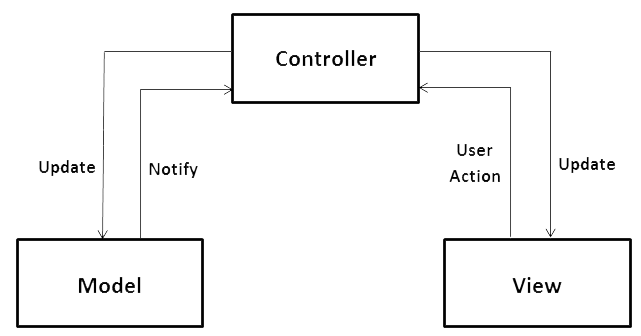
\includegraphics[width=0.6\textwidth]{Images/mvc}
\caption{Basic abstract overview of the Model-View-Controller pattern}
\end{figure}

\begin{itemize}
\item \textbf{Model} represents the underlying Ant Colony Optimisation algorithm. The Model also contains the required arithmetic functions and any additional operations required to execute the algorithm correctly.
\item \textbf{View} represents the graphical user interface which will not only display the algorithms execution, but also enable the user(s) to modify the algorithms parameters.
\item \textbf{Controller} represents the Observer required to enable interactions between the Model(s) and View(s).
\end{itemize}
\noindent


\subsection{Observer and Observable}

The implementation of the Model-View-Controller design pattern is handled using the Observer and Observable interface provided as part of the default Java language specification. The general premise is that the Model will have an Observer which will have an update interface allowing it to receive signals from what it is observing (Model). The Model will implement the Observable interface which will enable it to send update signals to the Observer through the notifyObservers() method. This enables the Models dependencies to be updated as the Model itself changes ensuring the correct state of the Model is captured in the Views.


\begin{figure}[h]
\centering
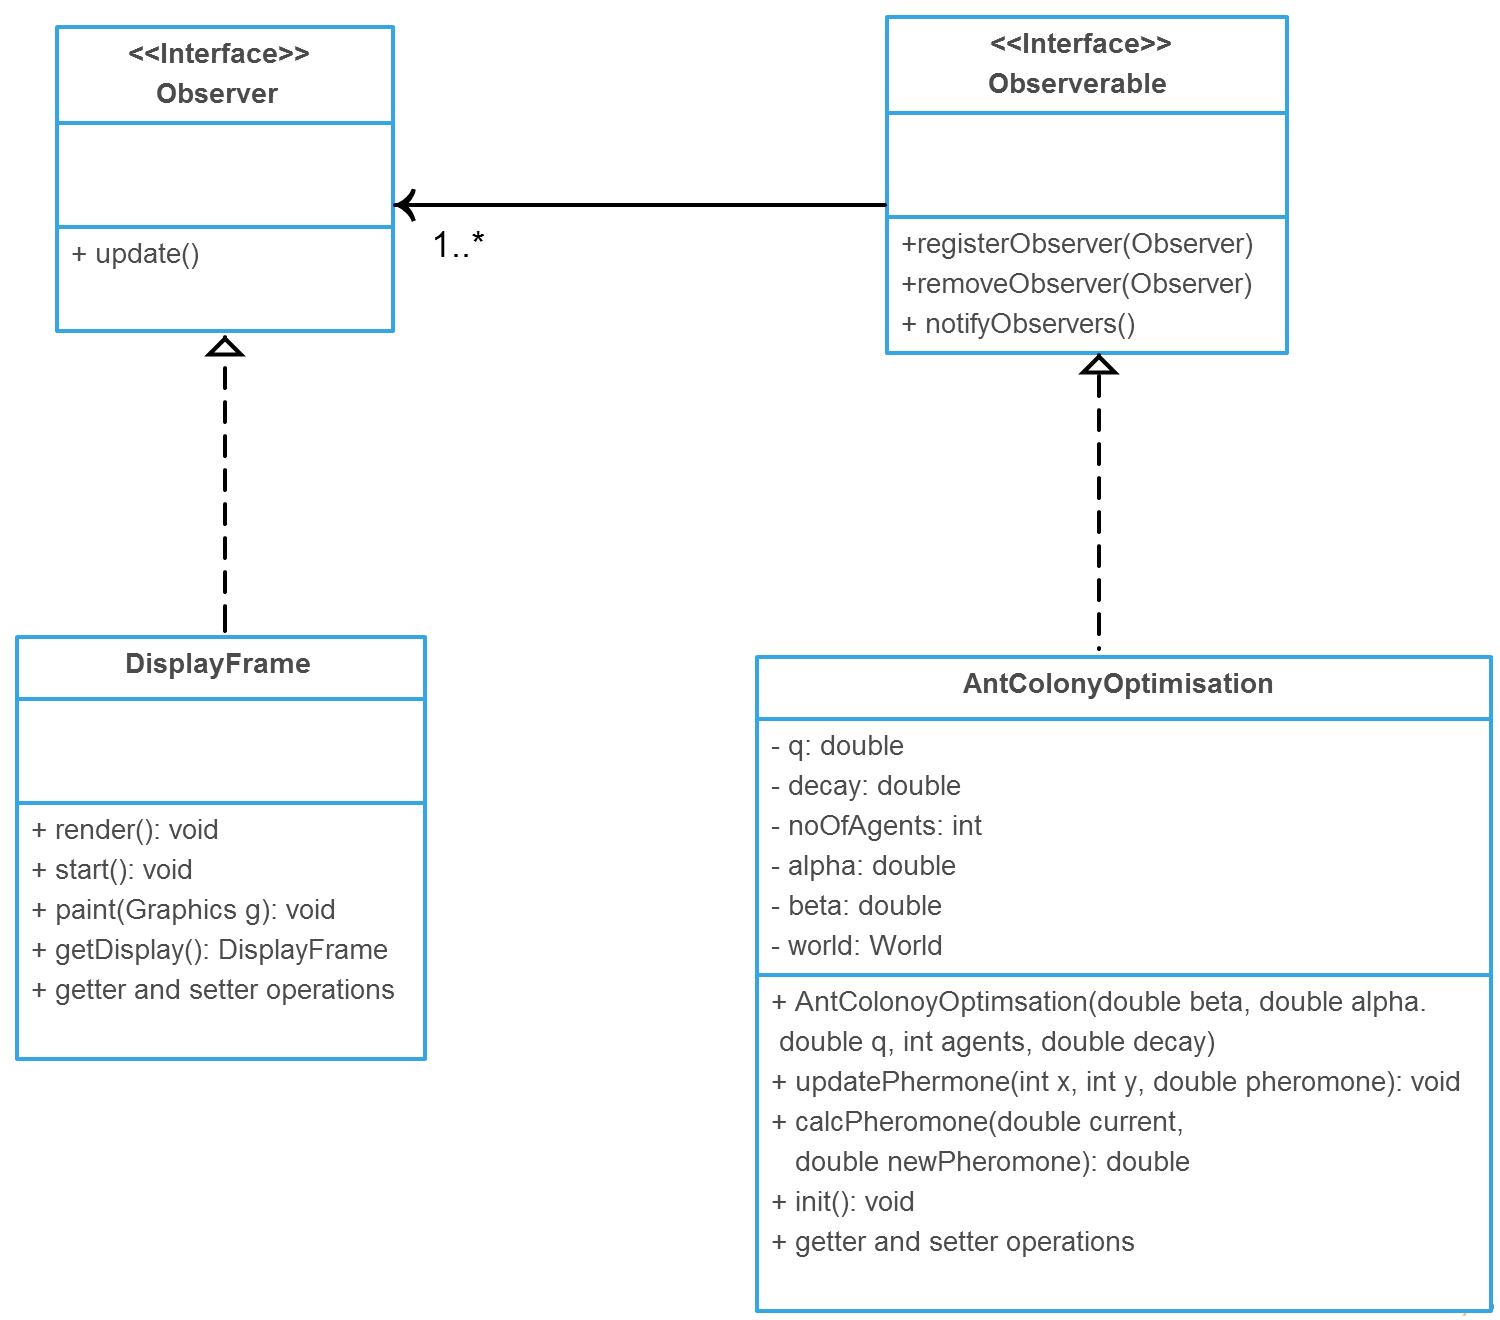
\includegraphics[width=0.9\textwidth]{Images/observer}
\caption{Proposed implementation of the Observer and Observable Design pattern}
\label{fig:observable}
\end{figure}

\noindent
As figure \ref{fig:observable} demonstrates the View will Observe the Model and will wait for an update signal sent by the Model's notifyObserver() method. The Model can have multiple Observers using this pattern so there is the potential for future modification or enhancement without having to rework the existing system should the needs for extra views be needed.

\subsubsection{Singleton}
\label{sssec:singleton}
In order to maintain simplicity throughout the application the Singleton design pattern will implemented for key Objects where one and only one instance of an Object must exist. The Singleton pattern prevents multiple instantiations of specific Object(s) as the Object itself is solely responsible for tracking the currently instantiated instance of itself\cite{gof:design:singleton}. 

The application will consist of a graphical user interface which in turn, will be composed of several different components. Such components must only be instantiated once in order to ensure correct interactions are performed. Without the presence of the Singleton pattern there exists the possibility of multiple instances of such components which could potentially cause unforeseen complications and undefined behaviours.

\begin{figure}[H]
\centering
\label{fig:singleton}
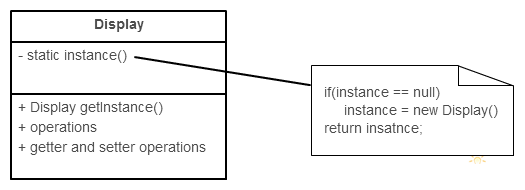
\includegraphics[width=0.8\textwidth]{Images/signleton}
\caption{Proposed high-level implementation of the Singleton pattern demonstrating how the sole instance of the graphical user interface will be tracked.}
\end{figure}

\subsection{Structure}

Adhering to the concepts of the patterns described in sections \ref{sssec:mvc} and \ref{sssec:singleton} the following Class Diagram shows proposed application structure. This is not concrete and could potentially change throughout development, the Class Diagram in question is represented below by figure \ref{fig:classdiagram} and is represented using standard UML notation.

\clearpage
\begin{sidewaysfigure}
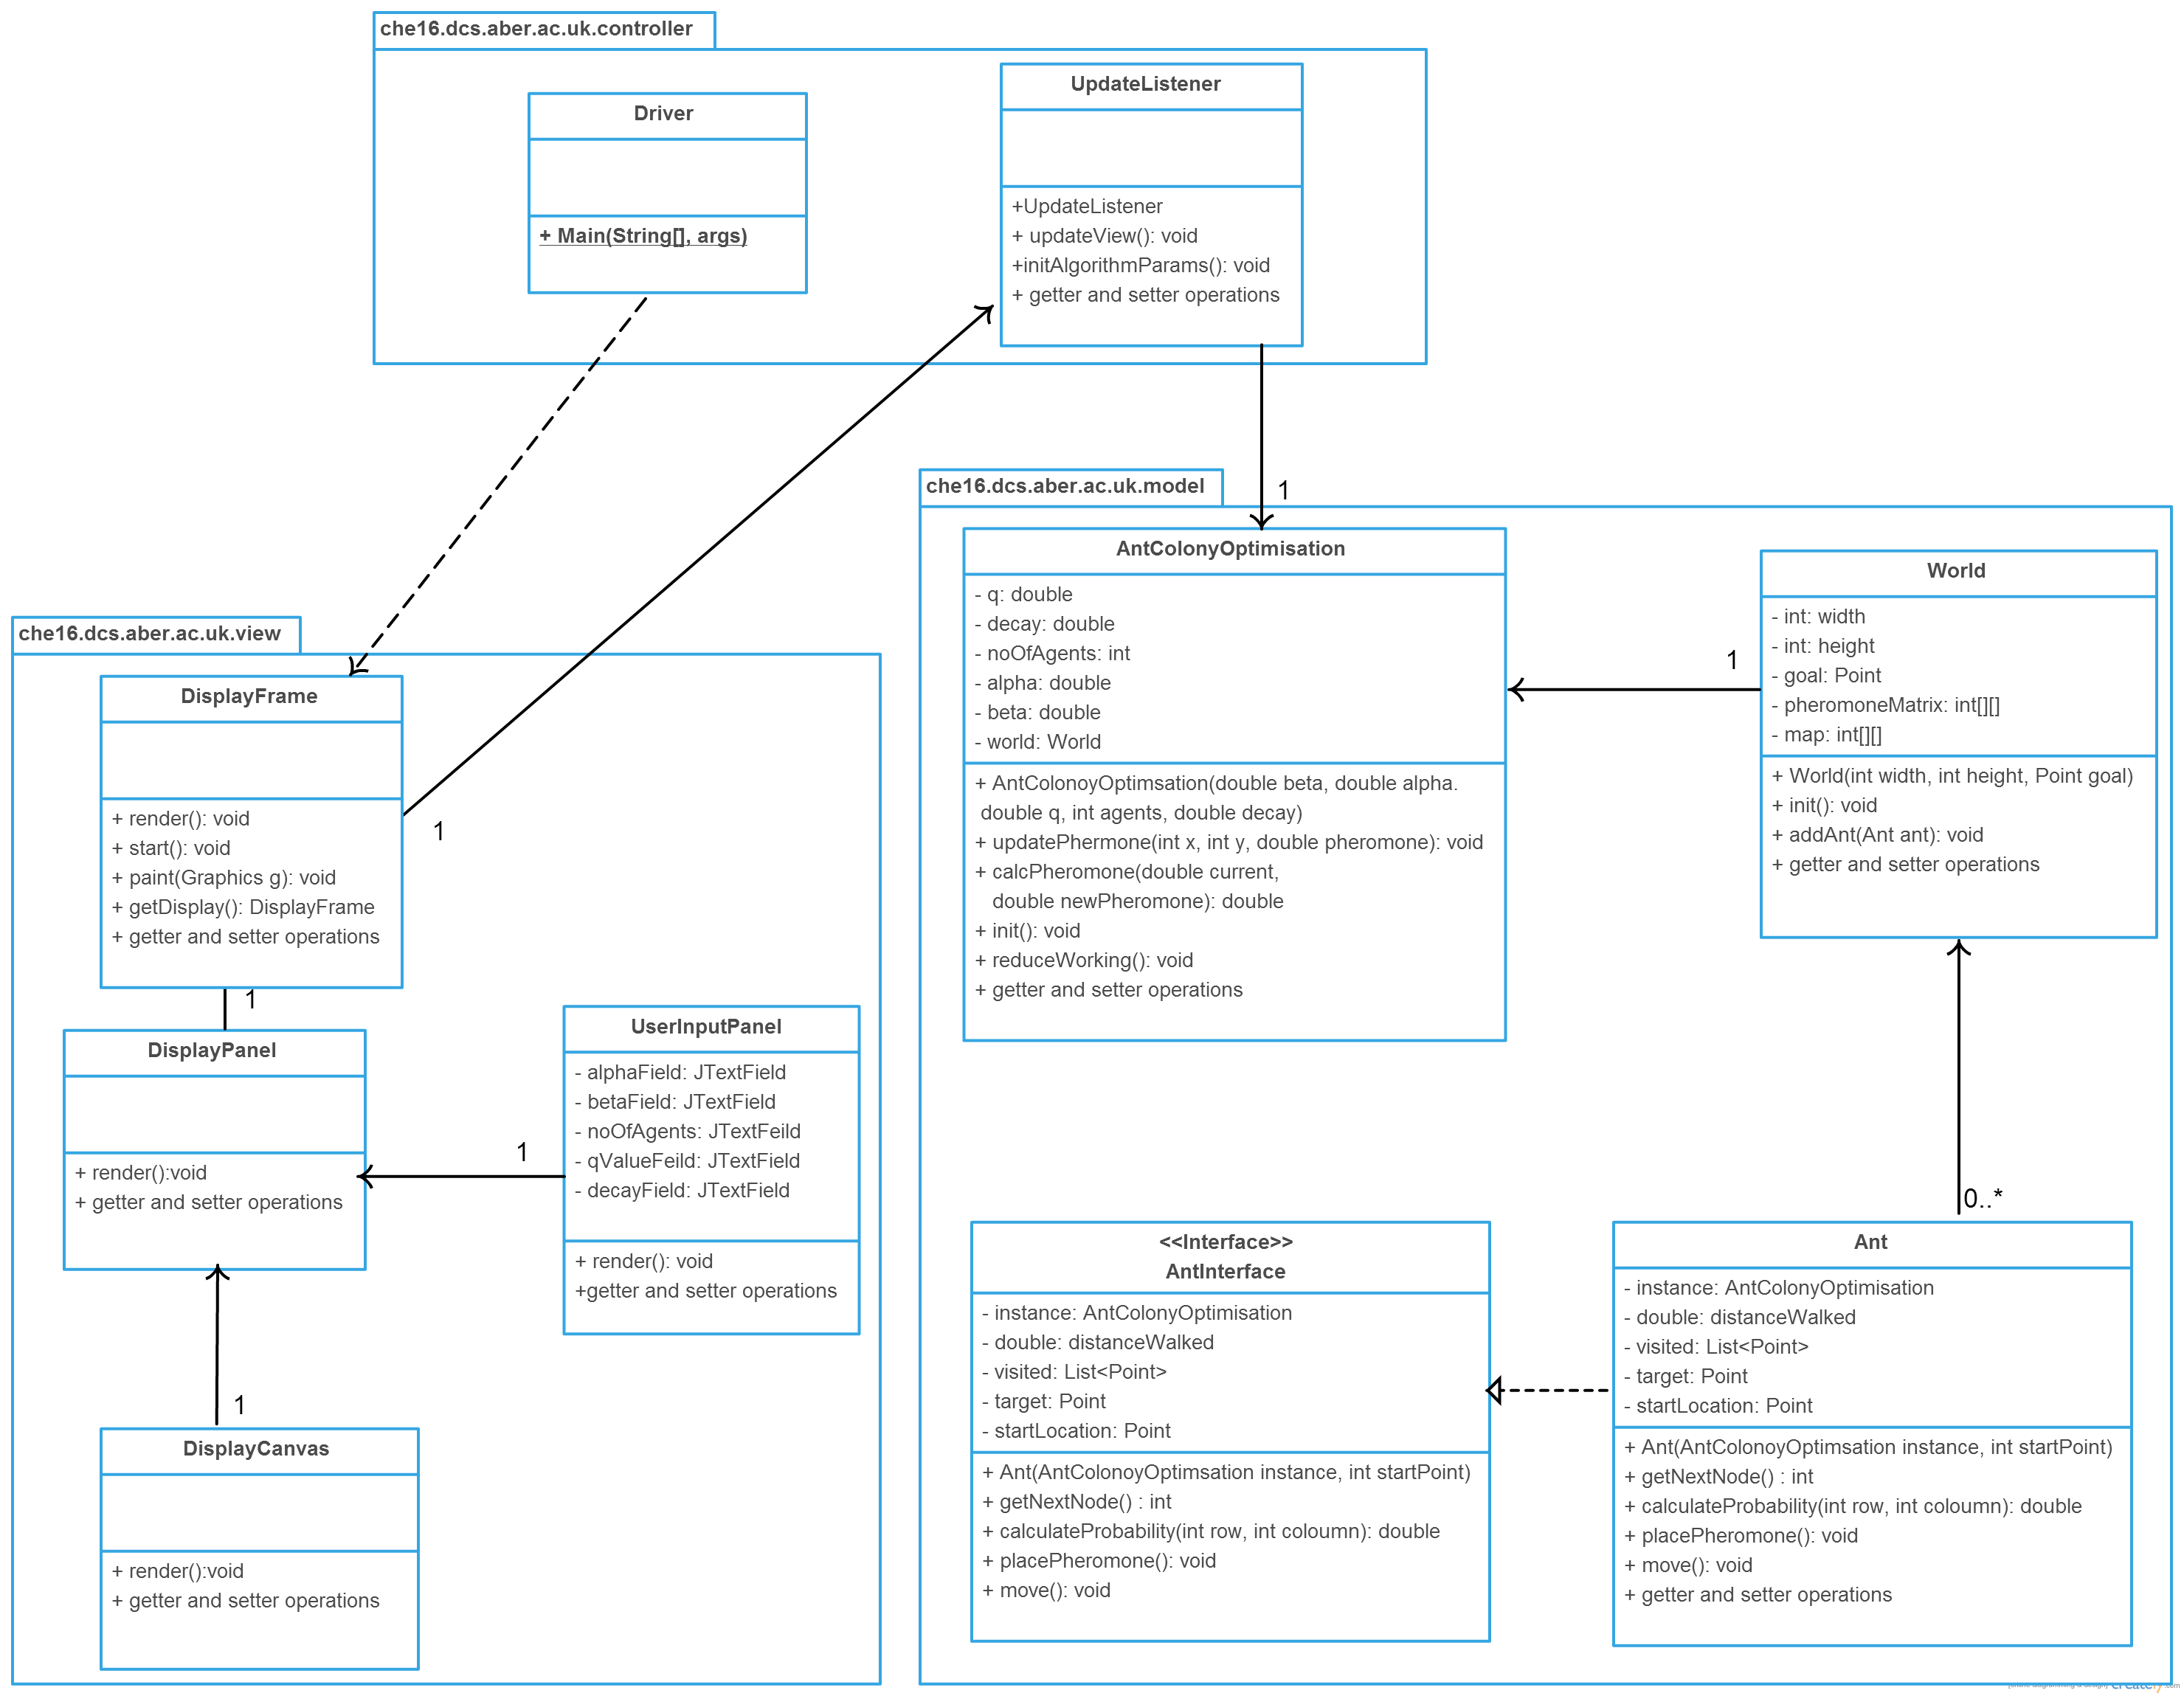
\includegraphics[scale=0.225]{Images/diss-uml}
\caption{Initial Class Diagram representing the main modules, packages and system interactions using UML notation.}
\label{fig:classdiagram}
\end{sidewaysfigure}
\clearpage

\subsubsection{View Package}

\label{sssec:view}
The $che16.dcs.aber.ac.uk.view$ package contains the graphical user interface components. The main concept behind this is the use of nested components such as JPanel, JTextFields and the like. These will be contained inside top level JFrame. This allows modification of each component in isolation without impacting the other components behaviours and/or elements. This is the first module of the application which is initialised, and is done so directly from the $main$ method. This package has no direct knowledge of any package members mentioned in \ref{sssec:model}. Instead the $che16.dcs.aber.ac.uk.controller$ package members handle the communication(s) between the model(s) and view(s), adhering to the principles discussed in section \ref{sssec:mvc}.

\subsubsection{Model Package}
\label{sssec:model}
The che16.dcs.aber.ac.uk.model package contains the necessary elements and attributes required in order to accurately represent the algorithms state(s) and ensure correct algorithm execution. This package has no directl knowledge of any package members mentioned in \ref{sssec:view}. Instead the controller package members handle the communication(s) between these the model(s) and view(s), adhering to the principles discussed in section \ref{sssec:mvc}.

\subsubsection{Controller Package}
The initial concept for the controller is basic and will grow in complexity during the development lifecycle as more and more control based mechanisms will become prevalent. This initial concept is a simple Observer which notifies the view(s) should the model change in a significant way; the inverse of this is also true.

\section{Interface Design}
\subsection{Main User Interface}
\label{ssec:mainUI}
The interface design must accommodate all the necessary elements required to allow user defined values for each of the algorithm parameters. The interface must also be able to visually represent the current algorithms state including the locations of the agents and nodes without impacting on the usability of the application (the interface must not freeze or be negatively affected by the algorithms execution).

The interface will use a very neutral colour scheme which will maximise the usability and reduce the risk of complications which may arise from users being subject to difficulties understanding or identifying certain colours. Every option for the user will be textually defined and will not rely on any sound or visual prompts in order to user. As a result in addition to the above, users with visual impairments will still be able to use the application as intended.

\begin{figure}[H]
\centering
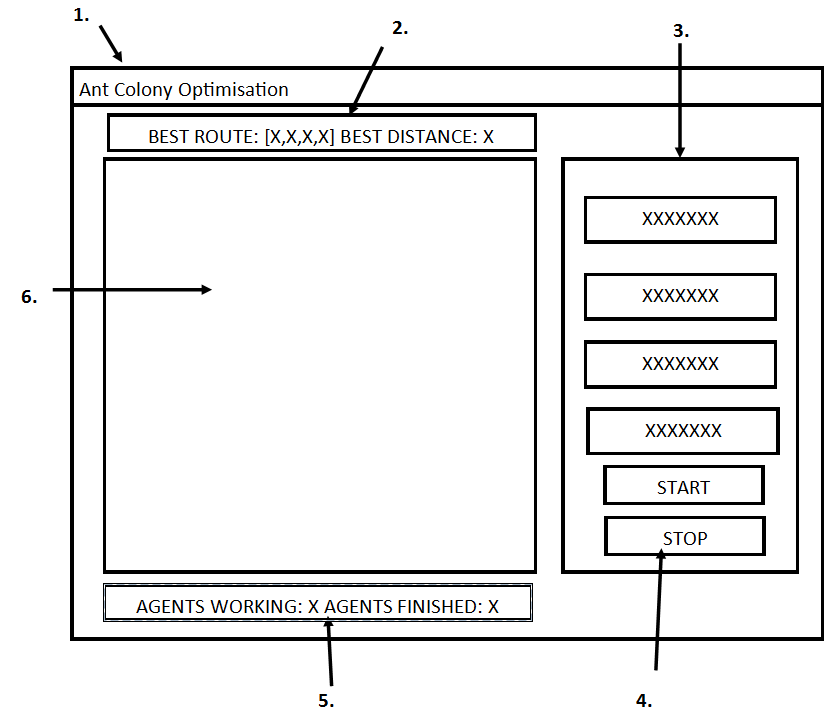
\includegraphics[width=0.8\textwidth]{Images/screen}
\caption{Proposed design for the graphical user interface, showing the key elements in their planned locations.}
\label{fig:interface}
\end{figure}

\noindent
\textbf{1.} in figure~\ref{fig:interface} refers to the containing frame which will house the reset of the interface elements. This frame will not be resizable preventing complications such as the dynamic resizing of the interface having an impact on the observable range of the world.
\noindent
\textbf{2.} in figure~\ref{fig:interface} refers to a text view containing information relevant to the algorithms current state of execution. This text view will contain the current best distance as well as the order of nodes visited to traverse the current best path. This will only be populated during the algorithms execution and only if the best path has been initialised.
\noindent
\textbf{3.} in figure~\ref{fig:interface} refers to container which houses the interactive elements relating to the modification of the algorithms parameters. This will consist of several labels and text fields which can be modified informing the user of what they will be modifying as well as providing suitable error messages if the users enters an incorrect value for any of the parameters.
\noindent
\textbf{4.} in figure~\ref{fig:interface} refers to the start and stop buttons. These are here to conform to the expectation that a user will expect some clear way to start and stop the application at their free choice, this is the simplest way to do this, and requires no hidden menus or hidden key bindings.
\noindent
\textbf{5.} in figure~\ref{fig:interface} refers to a text view containing information relevant to the algorithms current state of execution. This text view will contain the number of agents currently working (which means the number of agents who haven't met their own stop conditions) as well as displaying the number of agents which are finished.
\noindent
\textbf{6.}in figure~\ref{fig:interface} refers to the main canvas area which will display the algorithms current state of execution to the user. The contents of this will reflect the user defined values (elements in: \textbf{3.} in figure~\ref{fig:interface}) as well as representing each agents current location, their movements between nodes and also the modelling of pheromone deposit and decay will be present in this canvas.

\subsection{Error Message Feedback}

As the Algorithm parameters will be user defined using the interface proposed in section \ref{ssec:mainUI}, figure \ref{fig:interface} there must be measures in place to catch and inform the user of any illegal values. Not only must the user be told they have inputted illegal values the illegal parameter value will be identified and a range of legal values will be displayed to the user.

\begin{figure}[H]
\centering
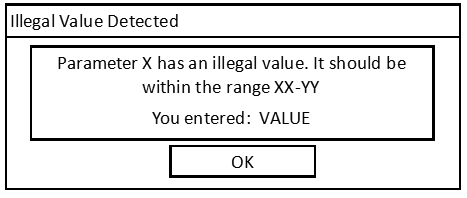
\includegraphics[width=0.8\textwidth]{Images/error}
\caption{Proposed design for the illegal parameter error message displayed to the user}
\label{fig:error}
\end{figure}

\noindent
As represented in figure \ref{fig:error} the error message will contain all the information a user needs to identify the problem with their data input. The X value in figure \ref{fig:error} represents which parameter has the illegal data input (i.e. Alpha, Beta). Range XX-YY represents the legal values for said parameter, and VALUE represents the value the user has specified for this parameter. The combination of these will provide the user with the knowledge of why this error message is being displayed and how they can resolve their issue.

This kind of error message will be composed using the JOptionPane and JDialog interfaces provided as default by the Java language specification. These views are very customisable and the styling will be handled by the languages underlying protocols which will reduce the codes complexity.

\section{Algorithm}

There are several adaptations of the Ant Colony Optimisation algorithm. Initially the project contain an implementation of Ant Colony Optimisation in its simplest form, without the presence of any enhancements such as using \textit{Elitist Agents} or similar. Once a working implementation is in place the next step will be to adapt the algorithm in various ways to further aid the teaching potential of the project.

The general premise is that each Agent (Ant) embarks and a pseudo random walk through the state space. The Agents movements are influenced by pheromone deposits placed on edges between vertices. This pheromone is deposited by other Agents in accordance with the equations stated in section \ref{sssec:pherodepo}. The Agent's next move is influenced by the result of the equation stated in section \ref{sssec:probfuncsssec}. However; there is still the probability of the Agent moving to a less attractive point so the Agent does not always travel to the strongest pheromone concentration.

Overtime the pheromone deposit concentration on $edge_{xy}$ is directly proportional to the quality of the candidate solution, and ultimately the ants will converge to find the shorted route between two or more points.

There are several algorithm requirements;
\begin{itemize}
\item \textbf{Suitable problem representation} the World and Agents must be represented in a suitable and logical manner allowing the algorithm to execute as expected.
\item \textbf{Pheromone manipulation metrics} there must exists adequate ways to access the pheromone matrix as well as manipulate (deposit/remove) the concentration of pheromone on a given edge in order to model decay and deposits.
\item \textbf{Probabilistic movement functions} there must exist functions that calculate the probability of the Agent moving to a specific vertex. This is based on the pheromone concentration and the Agent’s location (see section \ref{sssec:probfuncsssec}).
\end{itemize}

\clearpage
\begin{sidewaysfigure}
\centering
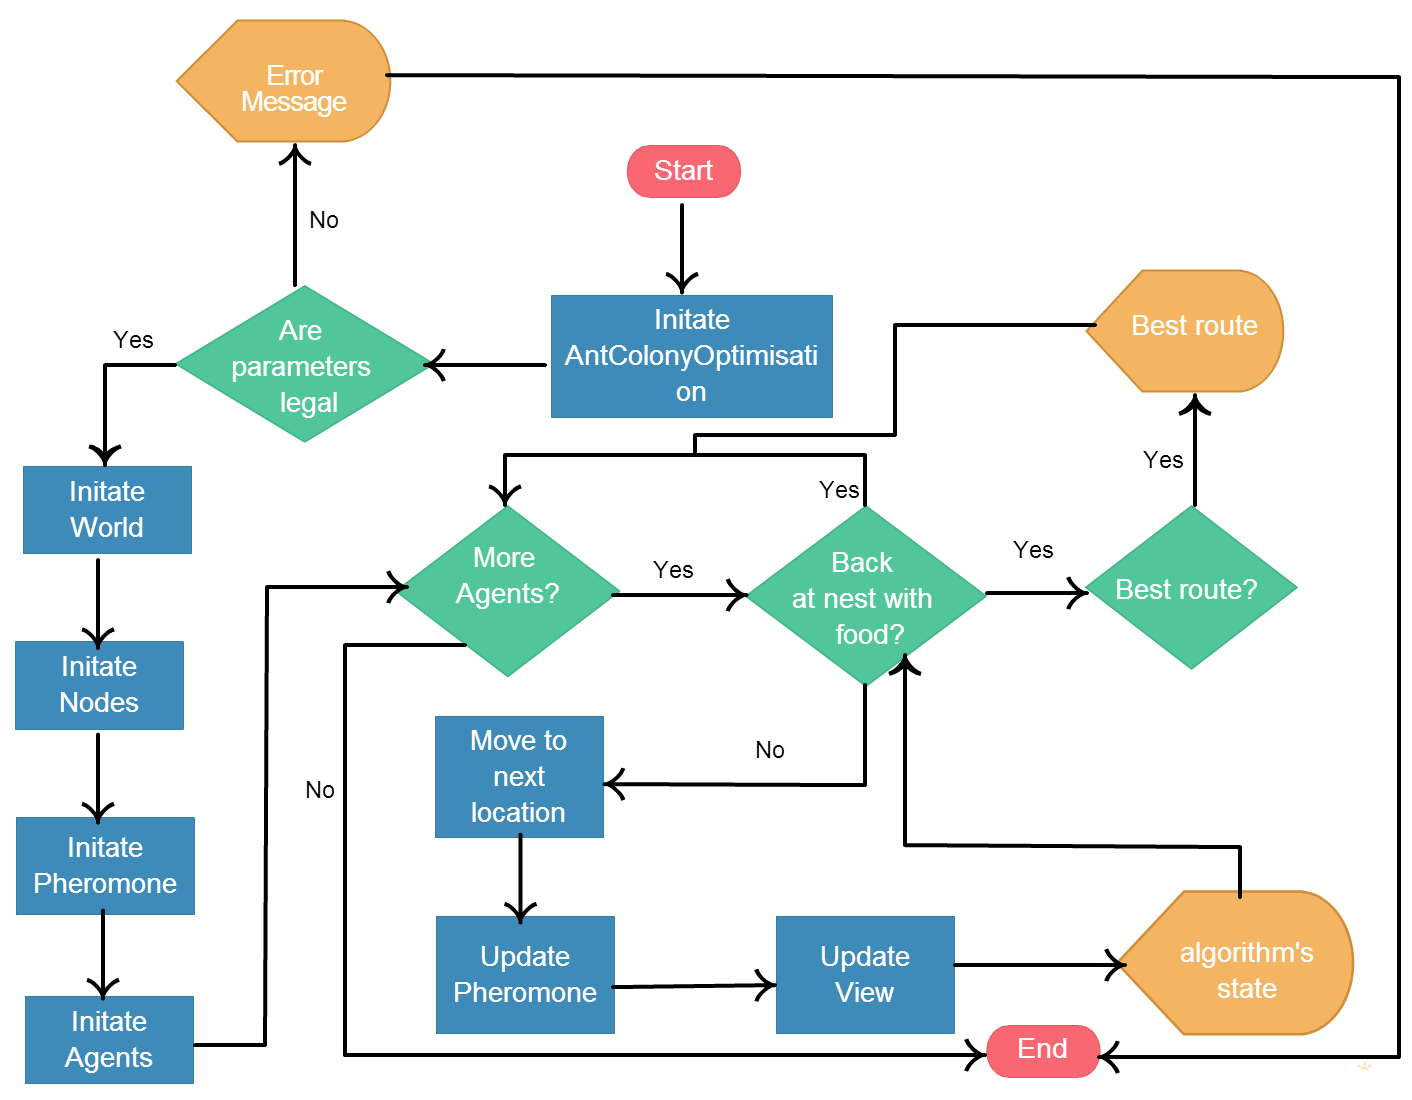
\includegraphics[scale= 0.45]{Images/flowmain}
\caption{High level flow digram representing the psudeo code for Algorithm \ref{aco:pseudo}, section \ref{sec:pseudo}}
\label{fig:interface}
\end{sidewaysfigure}
\clearpage

\subsection{Pseudo-code}
\label{sec:pseudo}
\begin{algorithm}
\caption{Pseudo-code for Ant Colony Optimisation}
\label{aco:pseudo}
\begin{algorithmic}[1]
\State Initiate AntColonyOptimisation with defined parameters
\If{$!parameters\ are\ legal$}
\State Dispaly error message to user
\State $return$
\EndIf
\State Initiate World with algorithm parameters
\State Initiate $Nodes$ and graph
\State Initiate \textit{pheromone} values
\State Initiate $Agents$
\While {$!all\ agents\ finished$} 
\ForAll{Agents}
\While{!back at $nest$ with $food$}
\State Calculate next move using probabilistic function 
\State Add moved point to Agent's memory
\State Calculate and deposit pheromone on the path
\State Update the View
\EndWhile 
\State \textbf{end while}
\EndFor 
\State \textbf{end for}
\EndWhile
\If{$\textit{local best solution} < \textit{global best solution}$}
\State $global best = local\ best\ solution$
\EndIf
\State \textbf{end if}
\State \textbf{end while}
\State output \textbf{global best} solution
\end{algorithmic}
\end{algorithm}

\noindent
Above is a somewhat simplified pseudo-code representation of the proposed Ant Colony Optimisation algorithm. The mathematical formulae required to achieve steps \textit{7} and \textit{10} are shown in section \ref{ssec:metrics}. The final algorithm may differ from the above depending on any additional feature present in the final release.

\clearpage
\begin{figure}
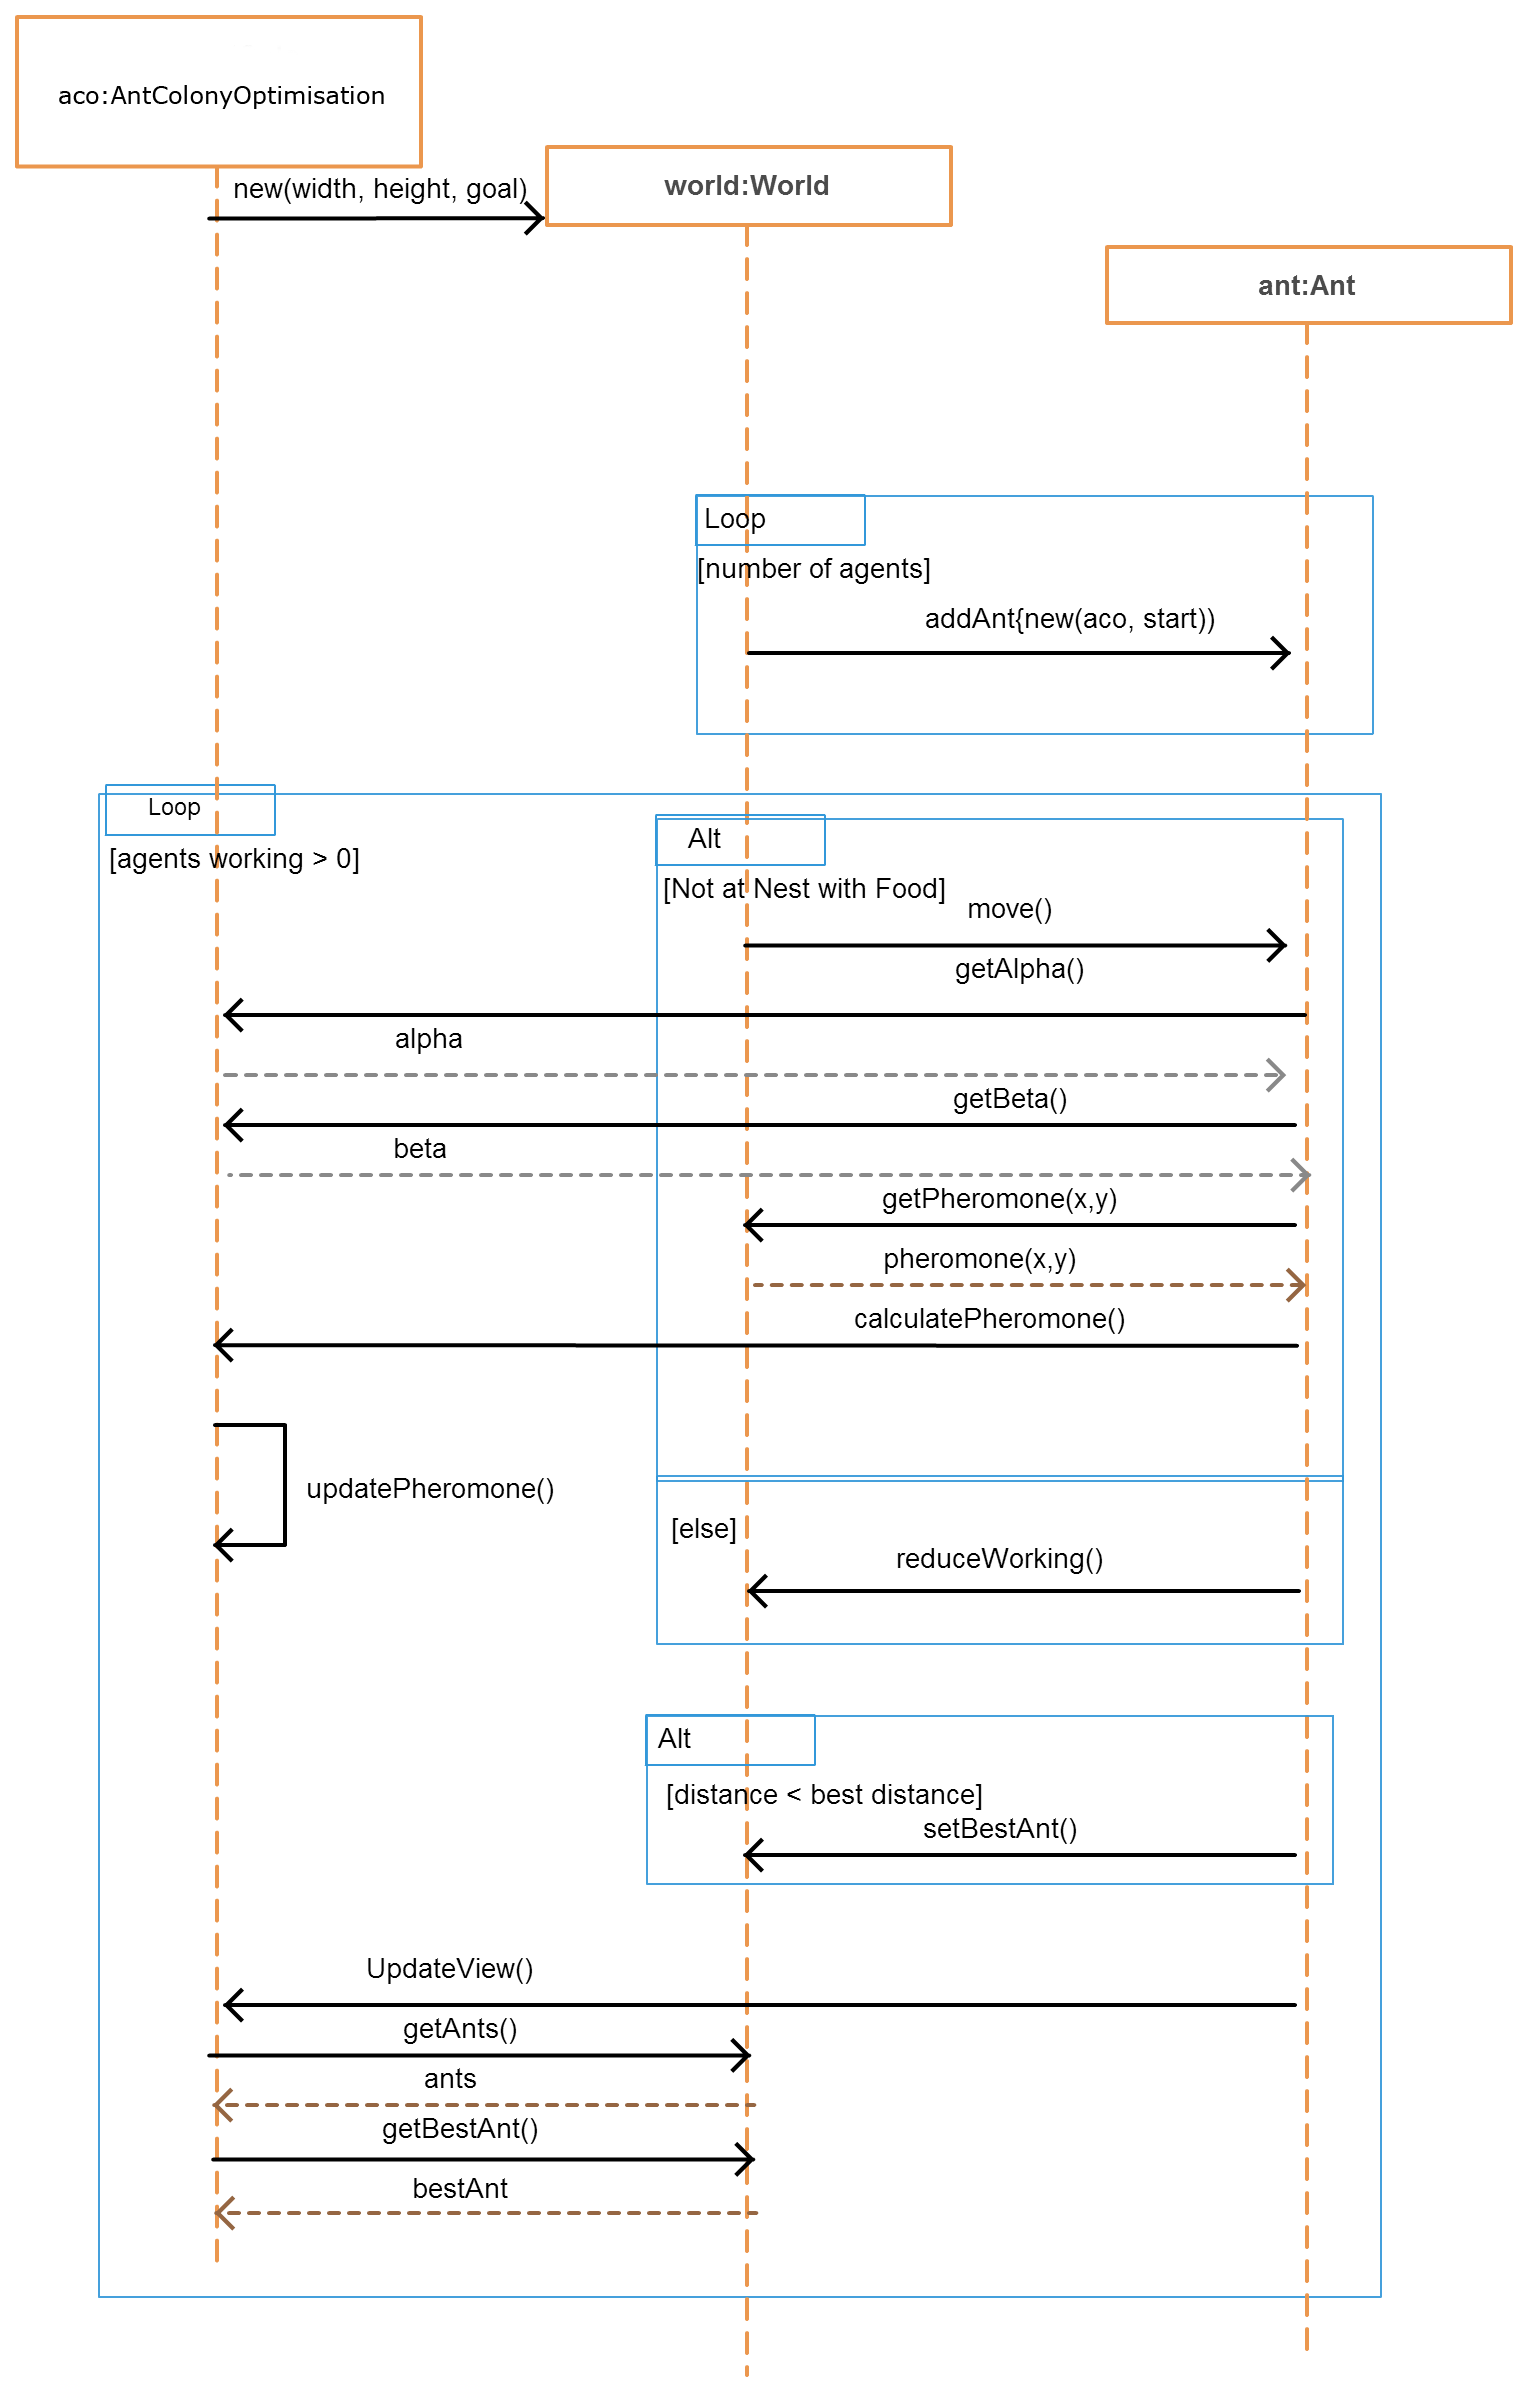
\includegraphics[scale = 0.3]{Images/sequenceRes}
\caption{Sequence diagram representing Algorithm \ref{aco:pseudo}, section \ref{sec:pseudo}}
\label{fig:seq}
\end{figure}
\clearpage

The sequence diagram shown in figure \ref{fig:seq} shows the high level interaction between the proposed main Model Classes during the algorithms execution. The Ants are in constant communication with the AntColonyOptimisation and World instances during their movement through the graph to ensure the correct pheromone values are being parsed during the movement process. The View is also updated through the updateView() method in the AntColonyOptimisation instance which requires data about the current Ants and the current best Ant. This data is stored in and returned from the World instance.

\subsection{Metrics}
\label{ssec:metrics}

\subsubsection{Probabilistic function}
\label{sssec:probfuncsssec}
\begin{figure}[H]
\Large
\begin{equation}
p_{xy}^{k} = \frac{(\tau_{xy}^{\alpha })(\eta _{xy}^{\beta })}{\sum (\tau_{xy}^{\alpha })(\eta _{xy}^{\beta })}
\end{equation}
\caption{Algebraic model of the probabilistic function used to calculate next move for any Agent \cite{probfunc:image}}
\label{fig:probfunc}
\end{figure}

\noindent
The probability that an Agent moves to vertex $xy$ is described using the above. $p$ is the probability for any Agent $k$ to move through vertex $xy$. $\tau$ is the amount of pheromone deposited on vertex $xy$, which is raised to the exponent $\alpha$. $\alpha$ is an heuristic value representing how greedy the algorithm is in its path finding \cite{tjung:aco:blog}. The result for $\tau_{xy}^{\alpha}$ is then multiplied by the edge $xy$'s evaluation($\eta$). Generally $\eta$ will be represented using $\frac{1}{Euclidean\ distance_{xy}}$\cite{tjung:aco:blog}\cite{sjored:Thesus2012}. This will then be raised to the exponent $\beta$ which like $\alpha$ is an heuristic parameter however $\beta$ describes the Agents path finding speed.$\sum (\tau_{xy}^{\alpha})(\eta_{xy}^{\beta})$ is the sum of all possible solutions.

\begin{algorithm}[H]
\caption{Pseudo-code for Probabilistic function - Each Agent - figure~\ref{fig:probfunc}}
\label{aco:pseudo:probfunc}
\begin{algorithmic}[1]
\State read the $pheromone$ level for vertex $xy$
\State raise the value from 1: to the exponent $\alpha$
\State Multiply the result of 2: by $(inverted\ distance_{xy})^{\beta}$ 
\State initiate a temporary double $cloumnTotal$
\ForAll{visted vertex}
\State $columnToal$ += (read the $pheromone$ level for vertex $xy)^{\alpha} \times $
$(inverted\ distance_{xy})^{\beta}$
\EndFor 
\State \textbf{end for}
\State divide the result of $3:$ by the result of $5:-7:$
\end{algorithmic}
\end{algorithm}

\subsubsection{Pheromone deposit}


\label{sssec:pherodepo}
\begin{figure}[H]
\Large
\begin{equation}
p_{xy}^{k} = (1 - \rho)\tau_{xy}^{k} + \Delta\tau_{xy}^{k}
\end{equation}

\caption{Algebraic model of the pheromone deposit function used to calculate the correct values for the pheromone matrix
\label{fig:pheromonefunc}
\cite{pheromone:image}}
\end{figure}

\noindent
$\tau$ represents the pheromone deposit for an edge $xy$ by Agent $k$ \cite{tjung:aco:blog}. $\rho$ is a value between $0-1$ which represents the decay rate $decay$. $1 - \rho$ is multiplied by the existing amount of pheromone at $edge_{xy}$ to correctly account for decaying trails. The new amount of pheromone is then added using the equation from figure~\ref{fig:newpheromonefunc}. 


\begin{figure}[H]
\Large
\begin{equation}
\Delta\tau_{xy}^{k} = 
\begin{dcases*}
Q/L_k & \text{if Agent $k$ uses curve $xy$ in its tour}\\
0 & \text{otherwise}
\end{dcases*}
\end{equation}

\caption{Algebraic model of the function used to calculate the how much new pheromone is deposited at $xy$
\label{fig:newpheromonefunc}
\cite{new:pheromone:image}. Pheromone is only updated if the Agent $k$ has visited point $xy$.}

\end{figure}

\noindent
figure~\ref{fig:newpheromonefunc} represents the new amount of pheromone to be added to the existing concentration at $edge_{xy}$. This can be read as change in $\tau\ (\Delta \tau)$. Q is simply another heuristic parameter which is divided by the distance $agent k$ travelled to get to $edge_{xy}$. If the result of this is $\leq 0$ return 0. This ensures that new $pheromone$ is only added to the existing concentration at $edge_{xy}$ is used by $agent k$ in its tour.

\begin{algorithm}[H]
\caption{Pseudo-code for Pheromone function - figures~\ref{fig:pheromonefunc}, \ref{fig:newpheromonefunc}}
\label{aco:pseudo:pherofunc}
\begin{algorithmic}[1]
\If {$pheromoneDeposit = Q\ value / totalDistanceWalked$ < 0}
\State $pheromoneDeposit = 0$
\EndIf
\State $pheromone_{xy}$ = (1 - $algorithm\ decay\ rate) \times currentPheromone_{xy} + pheromoneDeposit$
\If{$pheromone_{xy} \geq 0$}
\State $pheromoneMatrix_{xy} = pheromone_{xy}$
\Else
\State $pheromoneMatrix_{xy} = 0$
\EndIf \State \textbf{end if}
\end{algorithmic}
\end{algorithm}

\section{Representation}
\subsection{World}
\label{sec:world}
The World Class is used to model the graph that the Ants will traverse during the algorithms execution. The graph will be represented as a two-dimensional Array, with each element in said array representing a Node in the graph itself. The two dimensional array will be composed of integer values with each element containing an integer value representing the terrain type at this index, this will also be used to set the nest and food locations. 

\begin{figure}[H]
\centering
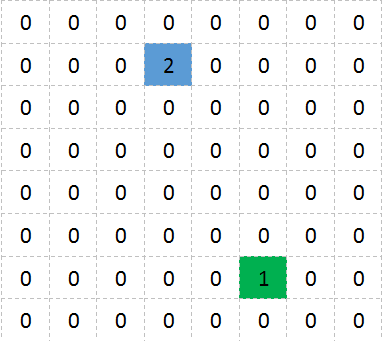
\includegraphics[scale=0.8]{Images/graph}
\caption{Example World representation using a two-dimensional Integer Array}
\label{fig:graph}
\end{figure}

\noindent
Figure \ref{fig:graph} shows how the proposed graph representation would be implement. A `0' value represents normal terrain where the Ants can move to, `1' represents the nest location where the Ants will start and `2' represents the food location which is the initial target for the Ants. This is a simplistic way to model an environment for the Ants whilst also allowing a multitude of terrain options without having to modify the way the graph is stored.

\subsection{Pheromone}
\label{pheroRepsec}
The pheromone must be modelled in a way which is both easily accessible and modifiable. The data structure used to store the pheromone must also relate to the graph mentioned in \ref{sec:world} to allow for logical mapping between the representation of the Ants environment and the pheromone associated with each Node in the graph. The pheromone will be stored as a two-dimensional Array of Doubles. Each element in the Array will represent the pheromone concentration for the corresponding Node in the graph for example, the double value at pheromone[x][y] will represent the pheromone concentration on edge [x][y] in the graph, thus there is a logical link between the two representations.

\begin{figure}[H]
\centering
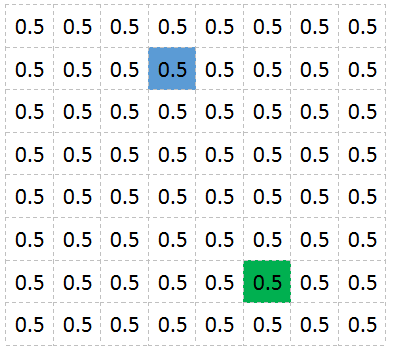
\includegraphics[scale=0.8]{Images/phero}
\caption{Example Pheromone representation using a two-dimensional Double Array with default initial values}
\label{fig:pheroRep}
\end{figure}

\noindent
Figure \ref{fig:pheroRep} demonstrates how a two-dimensional Double array can be effectively used to model the pheromone values for every Node in the graph. The values in this figure are default initial values which will be user defined when the application is executed. As the Ants moves through the graph the pheromone values at each index will correctly model the pheromone operations mentioned in section \ref{sssec:pherodepo}. As the values are stored in an array accessing or modifying the values is extremely simple and involves a simple getter or setter operation.

\subsection{Visualisation}

The data structures described in sections \ref{sec:world} and \ref{pheroRepsec} must be visualised to the user in a manner that anybody can understand. Given that the graph will be stored as a two-dimension array it is perfectly logical to display this graph to the user in a grid format similar to that shown in figure \ref{fig:graph}. The challenge with the visualisation process is visualising the pheromone deposit and decay operations as well as displaying the Ants moving between Nodes.

Given that the pheromone is stored in a two-dimensional array of doubles and the fact that accessing these values is extremely simple the value at each index can be used to directly influence how the user sees the pheromone. If each cell in the grid is coloured, and this colour's opacity is directly representational of the value at the corresponding index in the pheromone matrix then it becomes an accurate way of displaying the values of the pheromone to the user, which also allows the decay and deposit operations to be shown.

\begin{figure}[H]
\centering
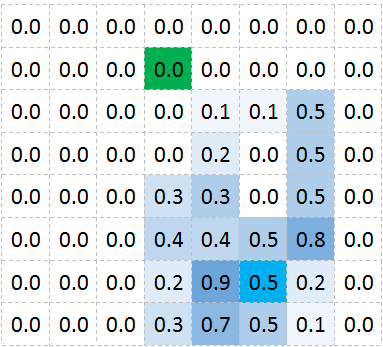
\includegraphics[scale=0.8]{Images/pheroEX}
\caption{Example Pheromone visualisation}
\label{fig:pheroVis}
\end{figure}

\noindent
Figure \ref{fig:pheroVis} shows how the pheromone value for a given [x,y] co-ordinate has a direct influence on the opacity of the cells colour. In said figure the pheromone value at each index is multiplied by 100 to convert it to a percentage, which then becomes the opacity value for the given Node. However, if the pheromone values for each Node become extremely small during execution there must be a measure in place to covert the small values back into percentages using a larger scaling factor than 100.


\clearpage
\chapter{Implemented Code}
\renewcommand{\thechapter}{\Alph{chapter}}

\begin{figure}[H]
\begin{lstlisting}
pheromone = new Pheromone[cities.size()][cities.size()];
	for(int i = 0; i < pheromone.length; i++){
		for(int j = 0; j < pheromone[0].length; j++){
			pheromone[i][j] = new Pheromone(aco.getInitialPheromone());
		}
	}
\end{lstlisting}
\caption{Snippet of code used to inialise the pheromone Matrix. $cities$ is a list of $City$ obejcts. $aco$ is the instance of the $AntColonyOptimisation$ Class}
\label{initPheroCode}
\end{figure}

\begin{figure}[H]
\begin{lstlisting}
distanceMatrix = new double[cities.size()][cities.size()];
	for(int i = 0; i < distanceMatrix.length; i++){
		for(int j = 0; j < distanceMatrix[0].length; j++){
			distanceMatrix[i][j] = Globals.calculateEuclidianDistance(cities.get(i).getX(), cities.get(i).getY(), cities.get(j).getX(), cities.get(j).getY());
		}
	}
\end{lstlisting}
\caption{Snippet of code used to inialise the distance Matrix. $cities$ is a list of $City$ obejcts.}
\label{initDistanceCode}
\end{figure}

\begin{figure}[H]
\begin{lstlisting}
invertedMatrix = new double[distanceMatrix.length][distanceMatrix[0].length];	
	for(int i = 0; i < distanceMatrix.length; i++){
		for(int j = 0; j < distanceMatrix[0].length; j++){
			invertedMatrix[i][j] = invertValue(distanceMatrix[i][j]);
		}
	}
\end{lstlisting}
\caption{Snippet of code used to inialise the inverted distance Matrix. $cities$ is a list of $City$ obejcts.}
\label{initInverteddistanceCode}
\end{figure}

\begin{figure}[H]
\begin{lstlisting}
cities = new ArrayList<City>();
	Random r = new Random();
	for(int i = 0; i < numberOfCities; i++){
		// the (+1) is to stop cities having the index '0' which would cause them to half render out of view
		int x = r.nextInt(aco.getBoundaryX()) + 1;
		int y = r.nextInt(aco.getBoundaryY()) + 1;
		//make sure 2 cities can't spawn on top of each other
		for(City city: cities){
			if(x == city.getX() && y == city.getY()){
				x = r.nextInt(aco.getBoundaryX()) + 1;
				y = r.nextInt(aco.getBoundaryY()) + 1;
			}
		}
		cities.add(new City(x,y,i));	
	}
\end{lstlisting}
\caption{Snippet of code used to inialise the collection of $City$ obejcts.}
\label{initCity}
\end{figure}

\begin{figure}[H]
\begin{lstlisting}
Random r = new Random();
	ants = new ArrayList<Ant>(numberOfAnts);
	for(int i = 0; i < numberOfAnts; i++){
		int index = r.nextInt(cities.size());
		for(City c: cities){
			if(index == c.getIndex()){
				c.adjustAntsHere(1);
				break;
			}
		}
		ants.add(new Ant(this, index));
	}
\end{lstlisting}
\caption{Snippet of code used to inialise the collection of $Ant$ obejcts.}
\label{initAnt}
\end{figure}

\begin{figure}[H]
\begin{lstlisting}
for(int i = 0; i < pheromone.length; i++){
		for(int j = 0; j < pheromone[0].length; j++){
			updatePheromone(i, j, pheromone[i][j].getNewPhero());
			//reset the new phero values
			pheromone[i][j].resetNewPhero();
		}
	}

public void updatePheromone(int x, int y, double newPheromone) {
	double phero = calculatePheromones(pheromone[x][y].getPheromoneValue(), newPheromone);
	//if phero is not negative then update the current concentration
	//if phero is negative then just set it as 0, you can't have negative phero on an edge
	if (phero >= 0.0d) {
		pheromone[x][y].setPheromoneValue(phero);
	} else {
		pheromone[x][y].setPheromoneValue(0.0d);
	}
}

public double calculatePheromones(double current, double newPheromone) {
	//we dont need to store the result in a temporary variable, just return the equation in place
	return ((1 - aco.getDecayRate()) * current + newPheromone);
}	
\end{lstlisting}
\caption{Snippet of code used to update the pheromone values for every edge.}
\label{codephero}
\end{figure}

\begin{figure}[H]
\begin{lstlisting}
public final int getNextProbableNode(int y) {
	//This is an adapted version of a similar method provided by Thomas Jungblut found here: https://code.google.com/p/antcolonyopt/
	//create a location to store the probability for all next locations
	//this can then be easily accessed to return the next index for the ant's move
	//only do this if there is in fact locations to move to
	if (unvisited > 0) {
		int danglingUnvisited = -1;
		final double[] weights = new double[visited.length];
		double columnSum = 0.0d;
		for (int i = 0; i < visited.length; i++) {
			columnSum += calculateIndividualProbability(y, i);
		}
		//once we have the value for sum (which the sum off all solutions evaluation)
		double sum = 0.0d;
		for (int x = 0; x < visited.length; x++) {
			if (!visited[x]) {
				weights[x] = calculateTotalProbability(x, y, columnSum);
				sum += weights[x];
				danglingUnvisited = x;
			}
		}
		//if sum is 0 then return, as this will be used in a division it cannot be zero
		if (sum == 0.0d)
			return danglingUnvisited;
		/*  We need to give each index of the probability weighting based on the result of calculateToalProbability
		 *  this result is then divided by the total sum of all probabilities (usually 1)
		 *  The result of this division is then put in the correct index in the matrix in order to get the probability weighting
		 *
		 */
		double pSum = 0.0d;
		for (int i = 0; i < visited.length; i++) {
			pSum += weights[i] / sum;
			weights[i] = pSum;
		}
		//nextDouble returns a value between 0 and 1, so this can be used to effectively select a 'random' index based on the weighted probability
		//provided virtually as is by Thomas Jungblut: https://code.google.com/p/antcolonyopt/
		//this is what makes the ant walk 'randomly'
		final double r = random.nextDouble();
		for (int i = 0; i < visited.length; i++) {
			if (!visited[i]) {
				if (r <= weights[i]) {
					return i;
				}
			}
		}
	}
	return -1;
}
\end{lstlisting}
\caption{Snippet of code used to select the Ants next location. This is a modifiedf version of the code provided by Thomas Jungblut \cite{tjung:aco:blog}}
\label{nextNodeCode}
\end{figure}

\begin{figure}[H]
\begin{lstlisting}
boolean reset = false;
for(int i = 0; i < iterations; i++){
		aco.setCurrentIteration(i);
		if(aco.getRunning()){
			ArrayList<Ant> ants = (ArrayList<Ant>)aco.getWorld().getAnts();
			antsWorking = aco.getNoOfAgents();
			if(reset){
				//for the next iteration re-init the ants and go again
				for(City c: aco.getWorld().getCities()){
					c.resetAntCount();
				}
				aco.getWorld().initAnts();
				ants = (ArrayList<Ant>)aco.getWorld().getAnts();
				reset = false;
				}
			while(antsWorking > 0){
				for(Ant ant: ants){
					if(!aco.getRunning()){
						return null;
					}
					if(!ant.getFinished()){
						ant.move();	
						aco.reduceWorking();
					}else{
						//if an ansst is finished, decrease the counter
						antsWorking--;
					}
				}
					aco.getWorld().decayPhero();
			}
			reset = true;
		}
	}
	
	
\end{lstlisting}
\caption{Snippet of code used to automatically execute the algorithm untill compeltion}
\label{iterationThing}
\end{figure}

\begin{figure}[H]
\begin{lstlisting}
if(currentIter < iterations){
		running = true;
		Ant ant = world.getAnts().get(stepIndex);
		if(!ant.getFinished()){
			ant.step();
			this.notifyCanvas();
			if(ant.getUnvisted() == 0){
				ant.setFinished(true);
			}
			}else{
			reduceWorking();
			stepIndex++;
		}
			if(stepIndex >= world.getAnts().size()){
			world.initAnts();
			for(City c: world.getCities()){
				c.resetAntCount();
			}
			stepIndex = 0;
			agentsWorking = noOfAgents;
			currentIter++;
		}
	}
\end{lstlisting}
\caption{Snippet of code used to execute the algorithm on a step by step basis}
\label{stepM8}
\end{figure}



\fancypagestyle{plain}{%
   \fancyhead{} %[C]{Annotated Bibliography}
   \fancyfoot[C]{{\thepage} of \pageref{LastPage}} % except the center
   \renewcommand{\headrulewidth}{0pt}
   \renewcommand{\footrulewidth}{0pt}
}

\setemptyheader

\nocite{*} % include everything from the bibliography, irrespective of whether it has been referenced.

% the following line is included so that the bibliography is also shown in the table of contents. There is the possibility that this is added to the previous page for the bibliography. To address this, a newline is added so that it appears on the first page for the bibliography. 
\addcontentsline{toc}{chapter}{Annotated Bibliography} % Adds References to contents page

%
% example of including an annotated bibliography. The current style is an author date one. If you want to change, comment out the line and uncomment the subsequent line. You should also modify the packages included at the top (see the notes earlier in the file) and then trash your aux files and re-run. 
%\bibliographystyle{authordate2annot}
\bibliographystyle{IEEEannot}
\renewcommand{\bibname}{Annotated Bibliography} 
\bibliography{References/references} % References file


\end{document}
